% ════════════════════════════════════════════════════════════════════════
%  Trabajo Fin de Grado — ETSIDI (UPM)
%  Plantilla original de Alberto Brunete (UPM), versión 3.
%  Sobre ella se han añadido sólo los paquetes que la memoria necesita
%  (unidades, tablas largas, diagramas y código); la estructura, los
%  márgenes y la portada son los de la plantilla.
%
%  Compilar:  latexmk -pdf TFG.tex     (pdfLaTeX + BibTeX)
%             tectonic TFG.tex         (sin instalar TeX Live)
%             o subir la carpeta a Overleaf
%
%  Las marcas \completar{...} (rojo) y \verificar{...} (naranja) señalan
%  lo que queda pendiente de rellenar o de comprobar en el montaje.
% ════════════════════════════════════════════════════════════════════════

\documentclass[10pt,a4paper]{book}

% ── Idioma y codificación ───────────────────────────────────────────────
\usepackage[spanish, es-tabla]{babel}
\usepackage{iftex}
\ifPDFTeX
  \usepackage[utf8]{inputenc}
  \usepackage[T1]{fontenc}
  \usepackage{lmodern}
  \usepackage{textcomp}
\else
  \usepackage{fontspec}
\fi

% ── Matemáticas y figuras (plantilla) ───────────────────────────────────
\usepackage{amsmath}
\usepackage{amsfonts}
\usepackage{amssymb}
\usepackage{graphicx}
\graphicspath{{figuras/}}
\usepackage{subfigure}
\usepackage{listings}
\usepackage{appendix}
\usepackage[left=3cm,top=3cm,right=3cm,bottom=3cm]{geometry}
\usepackage{multicol}

% ── Añadidos de esta memoria ────────────────────────────────────────────
\usepackage{siunitx}
\sisetup{output-decimal-marker={,}, group-separator={.}, per-mode=symbol,
         range-phrase={ a }, list-final-separator={ y }}
\DeclareSIUnit{\uacc}{u.a.}
\usepackage{booktabs}
\usepackage{longtable}
\usepackage{tabularx}
\usepackage{array}
\newcolumntype{L}[1]{>{\raggedright\arraybackslash}p{#1}}
\usepackage{float}
\usepackage[font=small,labelfont=bf]{caption}
\usepackage{enumitem}
\setlist{itemsep=2pt,topsep=4pt}
\usepackage{xcolor}
\usepackage{bytefield}
\usepackage{tikz}
\usetikzlibrary{arrows.meta,positioning,shapes.geometric,shapes.misc,fit,calc,backgrounds,babel}
\usepackage{pgfgantt}
\usepackage{xurl}
\usepackage{emptypage}
\raggedbottom

% ── Código ──────────────────────────────────────────────────────────────
\definecolor{codebg}{RGB}{247,247,247}
\definecolor{codecom}{RGB}{96,120,96}
\definecolor{codekw}{RGB}{30,60,150}
\definecolor{codestr}{RGB}{160,60,40}
\lstset{
  basicstyle=\ttfamily\footnotesize, backgroundcolor=\color{codebg},
  keywordstyle=\color{codekw}\bfseries, commentstyle=\color{codecom}\itshape,
  stringstyle=\color{codestr}, frame=single, rulecolor=\color{black!20},
  breaklines=true, columns=fullflexible, keepspaces=true, showstringspaces=false,
  numbers=left, numberstyle=\tiny\color{black!50}, xleftmargin=1.6em, framexleftmargin=1.4em,
  captionpos=b,
  literate={á}{{\'a}}1 {é}{{\'e}}1 {í}{{\'i}}1 {ó}{{\'o}}1 {ú}{{\'u}}1
           {Á}{{\'A}}1 {É}{{\'E}}1 {Í}{{\'I}}1 {Ó}{{\'O}}1 {Ú}{{\'U}}1
           {ñ}{{\~n}}1 {Ñ}{{\~N}}1 {ü}{{\"u}}1 {·}{{$\cdot$}}1 {→}{{$\rightarrow$}}1
           {←}{{$\leftarrow$}}1 {µ}{{$\mu$}}1 {°}{{$^\circ$}}1 {≤}{{$\le$}}1 {×}{{$\times$}}1
           {¿}{{?`}}1 {¡}{{!`}}1
}
\renewcommand{\lstlistingname}{Código}
\renewcommand{\lstlistlistingname}{Lista de \lstlistingname s}

% ── Enlaces ─────────────────────────────────────────────────────────────
\usepackage{hyperref}
\hypersetup{
    pdftitle={Banco de ensayos para una caracola de radio variable - TFG - 2026},
    pdfsubject={TFG - 2026},
    pdfauthor={Javier López},
    pdfkeywords={caracola} {tambor de radio variable} {Modbus RTU} {célula de carga},
    colorlinks, citecolor=black, filecolor=black, linkcolor=black, urlcolor=black,
}

% ── Macros del documento ────────────────────────────────────────────────
\DeclareRobustCommand{\completar}[1]{\textcolor{red!75!black}{\textbf{[COMPLETAR:} #1\textbf{]}}}
\DeclareRobustCommand{\verificar}[1]{\textcolor{orange!80!black}{\textbf{[VERIFICAR:} #1\textbf{]}}}
\newcommand{\codigo}[1]{\texttt{#1}}
\newcommand{\fichero}[1]{\texttt{#1}}
\newcommand{\ua}{u.\,a.}          % texto corrido; para \SI se usa \uacc
\newcommand{\autortfg}{Javier López \completar{segundo apellido}}

\begin{document}

\frontmatter

\begin{titlepage}
\begin{center}

 
\includegraphics[width=1\textwidth]{figuras/cabecera.png}  \\[0.5 cm]

\LARGE UNIVERSIDAD POLITÉCNICA DE MADRID \\ [1 cm]

\LARGE ESCUELA TÉCNICA SUPERIOR DE INGENIERÍA Y DISEÑO INDUSTRIAL \\ [1 cm]

\LARGE Grado en Ingeniería Electrónica y Automática Industrial\\ [1 cm]

\LARGE \textbf{TRABAJO FIN DE GRADO}\\[1 cm]

\huge \textsc{Banco de ensayos para una caracola de radio variable: control del
servoaccionamiento, adquisición de fuerza y validación del modelo}\\[1 cm]

\LARGE \autortfg \\[2 cm]

\begin{multicols}{2}
\begin{flushleft} \Large
\emph{Cotutor (si lo hay):} \completar{nombre y apellidos} \\
\emph{Departamento:} \completar{departamento}
\end{flushleft}

\begin{flushleft} \Large
\emph{Tutor:} \completar{nombre y apellidos}\\
\emph{Departamento:} \completar{departamento}
\end{flushleft}

\end{multicols}

\vfill

{\large Madrid, \completar{mes}, 2026}

\cleardoublepage


\thispagestyle{empty}

\includegraphics[width=1\textwidth]{figuras/cabecera.png}  \\[0.5 cm]

\LARGE UNIVERSIDAD POLITÉCNICA DE MADRID \\ [1 cm]

\LARGE ESCUELA TÉCNICA SUPERIOR DE INGENIERÍA Y DISEÑO INDUSTRIAL \\ [1 cm]

\LARGE Grado en Ingeniería Electrónica y Automática Industrial\\ [1 cm]

\LARGE \textbf{TRABAJO FIN DE GRADO}\\[1 cm]

\huge \textsc{Banco de ensayos para una caracola de radio variable}\\[3 cm]

\Large Firma del autor: \autortfg \\[3 cm]

\begin{multicols}{2}
\begin{flushleft}
\Large \emph{Firma del cotutor (si lo hay)}
\end{flushleft}

\begin{flushleft}
\Large \emph{Firma del tutor}
\end{flushleft}
\end{multicols}

\vfill
{\large Madrid, \completar{mes}, 2026}

\end{center}
\end{titlepage}
\normalsize


\begin{flushleft}

Copyright \copyright{} 2026. \autortfg

Esta obra está licenciada bajo la licencia Creative Commons Atribución-NoComercial-SinDerivadas 3.0
Unported (CC BY-NC-ND 3.0). Para ver una copia de esta licencia, visite
\url{http://creativecommons.org/licenses/by-nc-nd/3.0/deed.es} o envíe una carta a Creative Commons,
444 Castro Street, Suite 900, Mountain View, California, 94041, EE.UU.

\completar{confirmar la licencia que se quiere aplicar; ésta es la que propone la plantilla}

Todas las opiniones aquí expresadas son del autor, y no reflejan necesariamente las opiniones
de la Universidad Politécnica de Madrid.

\end{flushleft}


\cleardoublepage

\begin{flushleft} \large
\textbf{Título:} Banco de ensayos para una caracola de radio variable: control del
servoaccionamiento, adquisición de fuerza y validación del modelo \\
\textbf{Autor:} \autortfg\\
\textbf{Tutor:} \completar{nombre del tutor} \\
\textbf{Cotutor:} \completar{nombre del cotutor}\\ [1 cm]

\end{flushleft}

\begin{center} \LARGE
EL TRIBUNAL \\ [1 cm]
\end{center}

\begin{flushleft} \LARGE
Presidente: \\ [1 cm]
Vocal: \\ [1 cm]
Secretario: \\ [1.5 cm]
\end{flushleft}

\large
Realizado el acto de defensa y lectura del Trabajo Fin de Grado el día ....... de
....................   de ... en .........., en la Escuela Técnica Superior de Ingeniería y
Diseño Industrial de la Universidad Politécnica de Madrid, acuerda otorgarle la CALIFICACIÓN
de: \\ [2 cm]

\begin{center}
 \large VOCAL \\ [2.2 cm]
\end{center}

\begin{multicols}{2}
\begin{flushleft}
\large SECRETARIO
\end{flushleft}

\begin{flushleft}
\large PRESIDENTE
\end{flushleft}
\end{multicols}

\normalsize


\chapter{Agradecimientos}

\completar{Agradecimientos: tutoría, departamento o laboratorio que ha prestado el material,
compañeros y familia.}


\chapter{Resumen}

Este Trabajo Fin de Grado desarrolla el banco de ensayos de un mecanismo de elevación basado en una
\emph{caracola}: un tambor de radio variable que, accionado por un servomotor paso a paso de lazo
cerrado, enrolla un cable y levanta una barra articulada con una masa de \SI{2}{\kilo\gram}. La idea
que se quiere contrastar es la del \emph{fusee} de la relojería: si el radio del tambor crece donde
la tensión del cable es pequeña y decrece donde es grande, el par que ve el motor se mantiene
aproximadamente constante a lo largo del recorrido.

Para poder contrastarla se ha construido una plataforma completa: una placa adaptadora diseñada en
KiCad alrededor de una Raspberry Pi Pico~2, con bus RS-485, entradas digitales protegidas, entradas
analógicas acondicionadas, salidas de potencia y dos zócalos mikroBUS; un firmware en C++ que
gobierna el accionamiento por Modbus RTU, lee la célula de carga a través de un acondicionador
ZSC31014, hace el \emph{homing} con dos finales de carrera y ejecuta ciclos automáticos
B$\rightarrow$A$\rightarrow$B; un protocolo binario propio con CRC-8; y una aplicación web (FastAPI
y WebSocket) con tres páginas: monitor en tiempo real, configuración del mecanismo con simulador, y
visor de ensayos que superpone la curva teórica a cada medida.

El banco muestrea a \SI{20.0}{\hertz} con una dispersión del periodo de \SI{0.06}{\milli\second},
graba cada ensayo en cuentas brutas y repite el recorrido con una desviación típica de
\SI{11}{mrev} de motor. Se han analizado dos campañas de ensayos, la segunda con el
ciclo de ensayo reorganizado para que arranque en el extremo inferior del recorrido.

El resultado principal es metodológico y, en parte, negativo. El modelo estático reproduce bien la
forma de la señal de la célula de carga ($R^2 = 0{,}97$), pero se demuestra que esa comparación es
insuficiente: al no estar calibrada la célula, el ajuste absorbe un cambio de signo y el mismo
$R^2$ admite dos geometrías opuestas. El par del accionamiento, que no necesita calibración, deshace
la ambigüedad, y al hacerlo contradice la configuración vigente del mecanismo: sobre el tramo del
recorrido en que el cable trabaja con carga, el modelo predice que la tensión \emph{baja} un
\SI{20}{\percent} mientras que el par gravitatorio medido \emph{sube} un \SI{56}{\percent}. El radio
efectivo deducido crece un \SI{93}{\percent}, cuando para mantener el par constante bastaría con que
creciera un \SI{24}{\percent}. La caracola, tal y como está descrita en la configuración, no
compensa: sobrecompensa, y con el sentido invertido respecto del que pide el modelo.

El trabajo entrega, por tanto, un banco de ensayos reproducible, un modelo verificado en su
formulación y un procedimiento de contraste, junto con un diagnóstico claro de lo que falta para
cerrar la validación: medir las cotas reales del mecanismo y calibrar la célula con masas patrón.

\paragraph{Palabras clave:} tambor de radio variable, caracola, compensación de par, servomotor paso
a paso, Modbus RTU, RS-485, célula de carga, ZSC31014, Raspberry Pi Pico 2, adquisición de datos.

\chapter{Abstract}

This Bachelor's Thesis develops the test bench for a lifting mechanism based on a variable-radius
spiral drum (a \emph{fusee}-like drum, here called \emph{caracola}): driven by a closed-loop stepper
servomotor, it winds a cable that lifts a hinged bar carrying a \SI{2}{\kilo\gram} mass. The idea
under test is the one behind the horological fusee: if the drum radius grows where the cable tension
is small and shrinks where it is large, the motor torque stays roughly constant along the stroke.

A complete platform was built to test it: a KiCad-designed adapter board around a Raspberry Pi
Pico~2, with an RS-485 bus, protected digital inputs, conditioned analogue inputs, high-side outputs
and two mikroBUS sockets; C++ firmware that commands the drive over Modbus RTU, reads the load cell
through a ZSC31014 conditioner, performs homing with two limit switches and runs automatic
B$\rightarrow$A$\rightarrow$B cycles; a custom binary protocol with CRC-8; and a web application
(FastAPI and WebSocket) with three pages: real-time monitor, mechanism configuration with a
simulator, and a test viewer that overlays the theoretical curve on each measurement.

The bench samples at \SI{20.0}{\hertz} with a period spread of \SI{0.06}{\milli\second}, logs every
test in raw counts and repeats the stroke with a standard deviation of \SI{11}{mrev} of
motor shaft. Two test campaigns were analysed, the second one with the test cycle reorganised to
start at the lower end of the stroke.

The main result is methodological and partly negative. The static model reproduces the shape of the
load-cell signal well ($R^2 = 0.97$), but that comparison is shown to be insufficient: since the
cell is uncalibrated, the fit absorbs a sign change and the same $R^2$ admits two opposite
geometries. The drive torque, which needs no calibration, resolves the ambiguity --- and in doing so
contradicts the current configuration of the mechanism: over the loaded part of the stroke the model
predicts the tension to \emph{fall} by \SI{20}{\percent} while the measured gravitational torque
\emph{rises} by \SI{56}{\percent}. The implied effective radius grows by \SI{93}{\percent}, whereas
a \SI{24}{\percent} growth would suffice for constant torque. The spiral drum, as configured, does
not compensate: it overcompensates, and in the opposite sense to the one the model requires.

The thesis therefore delivers a reproducible test bench, a model verified in its formulation and a
contrast procedure, together with a clear diagnosis of what remains in order to close the
validation: measuring the real dimensions of the mechanism and calibrating the load cell with
reference masses.

\paragraph{Keywords:} variable radius drum, fusee, torque compensation, closed-loop stepper servo,
Modbus RTU, RS-485, load cell, ZSC31014, Raspberry Pi Pico 2, data acquisition.


\tableofcontents
\addcontentsline{toc}{chapter}{Índice}

\listoffigures

\listoftables

\chapter*{Acrónimos y símbolos}
\addcontentsline{toc}{chapter}{Acrónimos y símbolos}
\thispagestyle{plain}

\section*{Acrónimos}
\begin{longtable}{@{}L{0.18\textwidth}L{0.76\textwidth}@{}}
\toprule
\textbf{Sigla} & \textbf{Significado} \\
\midrule
\endhead
A/D, ADC & Convertidor analógico-digital (\emph{Analog-to-Digital Converter}) \\
API      & Interfaz de programación de aplicaciones \\
CDC      & Clase de dispositivo USB de comunicaciones (puerto serie virtual) \\
CRC      & Código de redundancia cíclica (\emph{Cyclic Redundancy Check}) \\
CSV      & Valores separados por comas (\emph{Comma-Separated Values}) \\
DE / RE  & Habilitación del emisor / receptor de un transceptor RS-485 \\
DI / DO  & Entrada digital / salida digital \\
EEPROM   & Memoria no volátil borrable eléctricamente \\
ESD      & Descarga electrostática (\emph{Electrostatic Discharge}) \\
FC       & Final de carrera \\
GPIO     & Entrada/salida de propósito general \\
GUI      & Interfaz gráfica de usuario \\
HTTP     & Protocolo de transferencia de hipertexto \\
I\textsuperscript{2}C & Bus serie síncrono de dos hilos (\emph{Inter-Integrated Circuit}) \\
LC       & Célula de carga (\emph{Load Cell}); LC1 y LC2 en el firmware \\
MISR     & Registro de firma de la EEPROM del ZSC31014 (\emph{Multiple-Input Signature Register}) \\
NC       & Contacto normalmente cerrado \\
ODS      & Objetivos de Desarrollo Sostenible \\
PCB      & Placa de circuito impreso (\emph{Printed Circuit Board}) \\
PIO      & E/S programable del RP2350 (\emph{Programmable I/O}) \\
POR      & Reinicio por encendido (\emph{Power-On Reset}) \\
RPM, rpm & Revoluciones por minuto \\
RS-485   & Estándar TIA/EIA-485 de transmisión diferencial multipunto \\
RTU      & Modo binario de Modbus sobre línea serie (\emph{Remote Terminal Unit}) \\
SMD      & Componente de montaje superficial \\
STO      & Desconexión segura del par (\emph{Safe Torque Off}) \\
TFG      & Trabajo Fin de Grado \\
UART     & Transmisor-receptor asíncrono universal \\
USB      & Bus serie universal \\
VRD      & Tambor de radio variable (\emph{Variable Radius Drum}) \\
WS       & WebSocket \\
\bottomrule
\end{longtable}

\section*{Símbolos principales}
\begin{longtable}{@{}L{0.17\textwidth}L{0.55\textwidth}L{0.16\textwidth}@{}}
\toprule
\textbf{Símbolo} & \textbf{Descripción} & \textbf{Unidad} \\
\midrule
\endhead
O         & Articulación de la barra & -- \\
D         & Punto por el que sale el cable hacia el tambor & -- \\
A         & Punto de la barra donde tira el cable & -- \\
$L_2$     & Altura de D sobre la articulación O & mm \\
$dx$      & Desplazamiento horizontal de D respecto de O & mm \\
$|OD|$    & Distancia de O a D, $\sqrt{L_2^2+dx^2}$ & mm \\
$L_3$     & Distancia de O al anclaje del cable en la barra & mm \\
$L_4$     & Distancia del anclaje al punto de suspensión de la masa & mm \\
$m$       & Masa suspendida & kg \\
$g$       & Aceleración de la gravedad & \si{\metre\per\second\squared} \\
$\alpha$  & Ángulo en O entre la línea O$\to$D y la barra, de 0° a 180° & ° \\
$\alpha_0$& Valor de $\alpha$ en B, donde arranca el ensayo & ° \\
$\theta$  & Ángulo de la barra respecto a la horizontal & ° \\
$c$       & Longitud libre de cable entre D y A & mm \\
$T$       & Tensión del cable & N \\
$\varphi$ & Giro del tambor contado desde B & rad \\
$r(\varphi)$ & Radio instantáneo de enrollamiento del tambor & mm \\
$s(\varphi)$ & Cable pagado por el tambor, $s=\int r\,\mathrm{d}\varphi$ & mm \\
$r_0$, $r_1$ & Radios de la caracola al principio y al final del barrido & mm \\
$\tau$    & Par en el eje del tambor & N·m \\
$N$       & Reducción motor:tambor (vueltas de motor por vuelta de tambor) & -- \\
$p$       & Avance del eje del motor contado desde B & rev \\
$\tau_g$, $\tau_f$ & Componentes gravitatoria y de pérdidas del par medido & \ua \\
$r_{\text{ef}}$ & Radio efectivo estimado, $\propto \tau_g/T$ & \ua/N \\
\ua       & Unidades internas del accionamiento (registro 16387) & -- \\
\bottomrule
\end{longtable}


\mainmatter

\chapter{Introducción}
\label{chap:intro}

\section{Motivación del proyecto}

Muchos mecanismos de elevación no presentan una carga constante al actuador. En una barra
articulada que se levanta tirando de un cable, la tensión necesaria para sostener la carga depende
del ángulo que forman el cable y la barra; al girar la barra, esa geometría cambia y con ella la
tensión. Si el cable se enrolla en un tambor cilíndrico, el par que el motor debe aportar, producto
de la tensión por el radio, sigue fielmente esas variaciones, y el actuador hay que dimensionarlo
para el peor punto del recorrido aunque la mayor parte del tiempo trabaje muy por debajo.

Una solución clásica es cambiar la relación de transmisión a lo largo del recorrido haciendo que el
radio del tambor no sea constante. Es la idea del \emph{fusee} de la relojería del siglo XV, un cono
con una ranura helicoidal que compensaba la pérdida de par del muelle real a medida que se
desenrollaba \cite{landes1983}. La misma idea reaparece hoy en los tambores de radio variable de la
robótica de cables \cite{seriani2016,bieber2023} y en los sistemas pasivos de compensación de
gravedad \cite{shen2022,endo2010}. En este trabajo, al tambor en espiral se le llama \emph{caracola}
por su forma.

El mecanismo objeto del proyecto es precisamente una caracola que, accionada por un servomotor paso
a paso de lazo cerrado, enrolla un cable y levanta una barra articulada con una masa de
\SI{2}{\kilo\gram}. La hipótesis de partida es que el perfil de radio variable aplana el par que ve
el motor frente a la variación de la tensión del cable. Comprobarlo exige dos cosas: un modelo que
diga qué cabe esperar y un sistema de medida capaz de registrar a la vez la posición del eje, la
tensión del cable y el par del motor en ensayos repetibles. Construir ese sistema, y usarlo para
contrastar el modelo, es el contenido de este Trabajo Fin de Grado.

\section{Objetivos}

El objetivo general es diseñar, construir y validar un banco de ensayos para el mecanismo de
caracola: la electrónica de accionamiento, control y adquisición, el software de supervisión y el
modelo con el que se interpretan las medidas.

De él se derivan los siguientes objetivos específicos:

\begin{enumerate}[label=\textbf{O\arabic*.}]
  \item Desarrollar un modelo estático del mecanismo que relacione la geometría, la tensión del
        cable y el par en el tambor, y deducir de él el perfil de radio que hace constante el par.
  \item Diseñar una placa de circuito impreso que adapte el microcontrolador al entorno de la
        máquina: bus RS-485, entradas digitales protegidas, entradas analógicas acondicionadas,
        salidas de potencia y conexión de células de carga.
  \item Desarrollar el firmware del microcontrolador, capaz de gobernar el servoaccionamiento por
        Modbus RTU, leer la célula de carga, ejecutar el \emph{homing} y los ciclos de ensayo, y
        vigilar los límites de seguridad con una temporización determinista.
  \item Definir un protocolo de comunicación robusto entre el microcontrolador y el ordenador, que
        transporte la telemetría por lotes y las órdenes con detección de errores.
  \item Desarrollar una aplicación de supervisión web para operar la máquina, visualizar los datos
        en tiempo real, grabar cada ensayo en un fichero reproducible, configurar la geometría del
        mecanismo y comparar cada ensayo con el modelo.
  \item Caracterizar el banco (temporización, repetibilidad y comportamiento de la medida) y
        analizar los ensayos para contrastar el modelo y cuantificar el efecto de la caracola.
  \item Documentar los problemas técnicos encontrados y las soluciones adoptadas, así como la
        planificación, el presupuesto y el impacto del trabajo.
\end{enumerate}

\section{Materiales utilizados}

\begin{itemize}
  \item \textbf{Mecanismo}: caracola de radio variable, cable, barra articulada con una masa de
        \SI{2}{\kilo\gram} y dos finales de carrera
        \completar{indicar si la caracola y la estructura se han diseñado y fabricado en este TFG o
        proceden de un trabajo previo}.
  \item \textbf{Accionamiento}: servomotor paso a paso de lazo cerrado con accionamiento Modbus RTU
        sobre RS-485 \completar{marca y modelo}.
  \item \textbf{Electrónica}: placa adaptadora propia diseñada en KiCad \cite{kicad} alrededor de un
        módulo Raspberry Pi Pico~2 \cite{rp2350}, con transceptor THVD1400 \cite{thvd1400},
        interruptor de potencia TPS4H000-Q1 \cite{tps4h000} y amplificadores MCP6294
        \cite{mcp629x}.
  \item \textbf{Medida de fuerza}: célula de carga con acondicionador ZSC31014 \cite{zsc31014}
        montado en una placa \emph{Load Cell 2 Click} \cite{mikroelc2}.
  \item \textbf{Software}: entorno Arduino con el núcleo Arduino-Pico \cite{arduinopico} y la
        biblioteca ModbusMaster \cite{modbusmaster} para el firmware; Python con FastAPI
        \cite{fastapi}, pySerial \cite{pyserial} y Chart.js \cite{chartjs} para la supervisión;
        matplotlib \cite{matplotlib} para el análisis, y git para el control de versiones.
\end{itemize}

\section{Alcance y limitaciones}

Entra en el alcance todo el sistema electrónico y de software (placa, firmware, protocolo,
supervisión y análisis), el modelo del mecanismo y la campaña de ensayos. El diseño mecánico se
toma como dado.

Las limitaciones conocidas, que se discuten en los capítulos correspondientes, son:

\begin{itemize}
  \item La posición del eje no se lee del codificador del accionamiento, sino que se obtiene
        integrando la velocidad que devuelve el propio servo (sección~\ref{sec:fw-posicion}).
  \item La célula de carga no está calibrada con masas patrón; los ensayos se guardan en cuentas
        brutas y la conversión a newtons es provisional (sección~\ref{sec:res-limitaciones}).
  \item El par se obtiene en las unidades internas del accionamiento, cuya escala física no se ha
        confirmado, de modo que los resultados se expresan en variaciones relativas.
  \item Las cotas del mecanismo no se han medido: los parámetros geométricos proceden de un ajuste
        sobre los propios ensayos (capítulo~\ref{chap:resultados}).
  \item Los finales de carrera y el límite de fuerza se implementan por software; no hay una cadena
        de seguridad cableada (sección~\ref{sec:arq-seguridad}).
\end{itemize}

\section{Metodología}

El desarrollo ha sido incremental y guiado por pruebas. Cada subsistema (bus RS-485, célula de
carga, finales de carrera, entradas y salidas de la placa) se validó primero con un programa de
prueba aislado, que se conserva en el repositorio (anexo~\ref{anx:repo}), antes de integrarlo en el
firmware principal. El código se ha versionado con git desde el primer día, y ese historial ha
servido además para reconstruir la planificación real (capítulo~\ref{chap:gestion}). Los ensayos se
guardan en crudo, con las constantes de conversión en la cabecera de cada fichero, de modo que
cualquier resultado puede recalcularse sin repetir el ensayo; las figuras de resultados de esta
memoria se generan con programas reproducibles a partir de esos ficheros.

\section{Estructura del documento}

\begin{itemize}
  \item El capítulo~\ref{chap:marco} resume los conceptos necesarios: accionamientos, medida de
        fuerza con galgas, buses de campo y microcontroladores.
  \item El capítulo~\ref{chap:estado} sitúa el trabajo frente a los tambores de radio variable y los
        mecanismos de compensación publicados.
  \item El capítulo~\ref{chap:modelo} desarrolla el modelo del mecanismo y el método experimental
        con el que se contrasta.
  \item El capítulo~\ref{chap:arquitectura} recoge los requisitos y la arquitectura del banco.
  \item Los capítulos~\ref{chap:hardware} a~\ref{chap:software} describen el hardware, el firmware,
        las comunicaciones y el software de supervisión.
  \item El capítulo~\ref{chap:problemas} reúne los problemas técnicos y sus soluciones.
  \item El capítulo~\ref{chap:resultados} presenta la caracterización del banco y los resultados de
        las dos campañas de ensayos.
  \item El capítulo~\ref{chap:gestion} trata el ciclo de vida, la planificación y el presupuesto, y
        el capítulo~\ref{chap:conclusiones} las conclusiones y el trabajo futuro.
\end{itemize}

Los anexos contienen la asignación de pines, el protocolo, los registros Modbus, el formato de los
ficheros de ensayo, el manual de uso y la estructura del repositorio.


\chapter{Marco teórico}
\label{chap:marco}

Este capítulo resume los conceptos necesarios para seguir el resto de la memoria: cómo se acciona
el eje, cómo se mide la fuerza, con qué microcontrolador y por qué buses viaja la información.

\section{Transmisión por cable y radio variable}

En una transmisión por cable, el par que hay que aplicar al tambor es el producto de la tensión del
cable por el radio con el que ese cable sale del tambor:
\begin{equation}
  \tau = T\,r .
  \label{eq:par-basico}
\end{equation}
Si el radio es constante, el par reproduce exactamente la forma de la tensión. Si el radio cambia
con el giro, $r(\varphi)$, se dispone de un grado de libertad para moldear el par: basta con que el
radio sea grande donde la tensión es pequeña, y pequeño donde es grande, para que el producto se
mantenga aproximadamente constante. Ésa es la idea del \emph{fusee} y de los tambores de radio
variable, y el capítulo~\ref{chap:modelo} la desarrolla para la geometría concreta del prototipo.

Conviene separar dos cosas que se confunden con facilidad. Un mecanismo de compensación
\emph{pasiva} (un muelle con una polea no circular) reduce la energía que el actuador tiene que
aportar. Una caracola accionada por un motor no reduce esa energía: el trabajo de subir la masa es
el mismo. Lo que hace es repartirlo de manera uniforme a lo largo del giro, lo que reduce el par de
pico y, con él, el tamaño del motor necesario.

\section{Accionamiento: servomotores paso a paso de lazo cerrado}

Un motor paso a paso convencional funciona en lazo abierto: el controlador impone la secuencia de
fases y se da por hecho que el rotor la sigue. Es sencillo y tiene buen par a baja velocidad, pero
si la carga supera el par disponible se pierden pasos sin que el sistema lo detecte
\cite{kenjo1994}. Los servomotores paso a paso de lazo cerrado añaden un codificador y un
accionamiento que regula la corriente en función del error de posición: conservan el par a baja
velocidad, no pierden pasos y ofrecen modos de control en posición, velocidad o par, además de
magnitudes de supervisión como la velocidad real o el par entregado.

El accionamiento de este trabajo pertenece a esa familia \completar{marca y modelo del motor y del
accionamiento, par nominal, tensión de alimentación y resolución del codificador}. Integra una
interfaz RS-485 con protocolo Modbus RTU, por la que se configura (modo de control, rigidez, rampas
y resistencia de frenado), se habilita, se envía la consigna de velocidad y se leen la velocidad y
el par. Tenerlo todo en un bus de dos hilos simplifica el cableado frente a la alternativa de
señales de paso y dirección más entradas analógicas.

\section{Medida de fuerza con células de carga}

\subsection{Galgas extensométricas y puente de Wheatstone}

Una célula de carga convierte la fuerza en una deformación elástica, que se mide con galgas
extensométricas dispuestas en un puente de Wheatstone \cite{hoffmann2012}. La salida del puente es
una tensión diferencial de unos pocos milivoltios por voltio de excitación a plena escala, que hay
que amplificar con alta ganancia y bajo ruido antes de digitalizarla; además hay que compensar el
desequilibrio de cero del puente y su deriva con la temperatura \cite{pallas2001}. De ahí que la
cadena de medida necesite, ante todo, una calibración con masas patrón: sin ella se conoce la forma
de la señal, pero no su escala ni su cero.

\subsection{Acondicionadores integrados}

Existen circuitos integrados que agrupan excitación, amplificación, conversión A/D y corrección
digital. En este trabajo se han evaluado dos:

\begin{itemize}
  \item \textbf{ZSC31014} de Renesas \cite{zsc31014}, con salida digital I\textsuperscript{2}C,
        preamplificador de ganancia programable, conversor de 14 bits y corrección almacenada en
        EEPROM. Cada lectura incluye dos bits de estado que indican si el dato es nuevo. Su
        configuración sólo puede modificarse en un \emph{modo comando} al que se accede durante una
        ventana corta tras el encendido, lo que ha condicionado el diseño
        (sección~\ref{sec:prob-zsc}). Se usa en una placa \emph{Load Cell 2 Click}
        \cite{mikroelc2}.
  \item \textbf{NAU7802} de Nuvoton \cite{nau7802}, conversor sigma-delta de 24 bits con
        amplificador programable y regulador interno. Se probó como segunda célula y se retiró del
        firmware final.
\end{itemize}

\section{Microcontrolador}

El proyecto empezó con una placa basada en ESP32-S3 (Seeed XIAO) y se migró a una Raspberry Pi
Pico~2. La tabla~\ref{tab:mcu} resume las características del RP2350 \cite{rp2350}. El motivo del
cambio y sus consecuencias se explican en la sección~\ref{sec:prob-uart}: los pines que impone el
trazado de la placa no admiten una UART hardware, pero el RP2350 dispone de periféricos PIO capaces
de implementar una UART en cualquier pin.

\begin{table}[H]
\centering
\caption{Características del microcontrolador RP2350 en la Raspberry Pi Pico 2 \cite{rp2350}.}
\label{tab:mcu}
\begin{tabular}{@{}ll@{}}
\toprule
Característica & Raspberry Pi Pico 2 (RP2350) \\
\midrule
Núcleos & 2 × Arm Cortex-M33 o 2 × RISC-V Hazard3, a \SI{150}{\mega\hertz} \\
Memoria & \SI{520}{\kilo\byte} SRAM, \SI{4}{\mega\byte} flash QSPI \\
Periféricos serie & 2 × UART, 2 × SPI, 2 × I\textsuperscript{2}C \\
E/S programable & 12 máquinas de estado PIO \\
Entradas analógicas & 3 canales ADC \\
Entorno usado & Arduino-Pico \cite{arduinopico} \\
\bottomrule
\end{tabular}
\end{table}

\section{Buses de comunicación}

\subsection{RS-485 y Modbus RTU}

RS-485 \cite{tia485} es un estándar de capa física diferencial y multipunto, extendido en la
industria por su inmunidad al ruido, su alcance y la posibilidad de conectar varios equipos al mismo
par trenzado. En modo semidúplex cada nodo activa su emisor sólo mientras transmite, y ese control
de dirección (líneas DE y $\overline{\text{RE}}$ del transceptor) corresponde al maestro.

Modbus \cite{modbusapp} es un protocolo maestro-esclavo de petición y respuesta que modela los datos
del esclavo como registros de 16 bits. En su variante RTU sobre línea serie \cite{modbusserial},
cada trama lleva la dirección del esclavo, el código de función, los datos y un CRC-16, y las tramas
se delimitan por silencios de al menos 3,5 caracteres. Aquí se usan la función 0x03 (lectura de
registros) y la 0x06 (escritura de un registro), a través de la biblioteca ModbusMaster
\cite{modbusmaster}.

\subsection{I\textsuperscript{2}C y mikroBUS}

I\textsuperscript{2}C \cite{i2cspec} es un bus síncrono de dos hilos con resistencias de
\emph{pull-up}, pensado para comunicar circuitos dentro de una misma placa; es el que usan los
acondicionadores de célula de carga. Las placas Click siguen el estándar mikroBUS \cite{mikrobus},
que define un zócalo de 16 pines con I\textsuperscript{2}C, SPI, UART, alimentación y señales
auxiliares.

\section{Adquisición y supervisión en el ordenador}

La supervisión de máquinas se ha hecho tradicionalmente con paneles HMI o paquetes SCADA
comerciales. Para un banco de laboratorio, una aplicación web local es una alternativa ligera: no
requiere licencias, funciona en cualquier navegador y admite varios clientes a la vez. En este
trabajo se emplea FastAPI \cite{fastapi} con pySerial \cite{pyserial} para el puerto USB, WebSocket
\cite{rfc6455} para el envío continuo de datos al navegador y Chart.js \cite{chartjs} para las
gráficas.

Dos conceptos de adquisición son importantes para interpretar los resultados. El primero es la
\emph{base de tiempos}: si las muestras se marcan con el reloj del ordenador, la latencia del enlace
se confunde con el fenómeno medido; por eso aquí cada muestra lleva la marca de tiempo del
microcontrolador. El segundo es la distinción entre \emph{dato bruto} y \emph{dato calibrado}:
guardar las cuentas del conversor, y no los newtons, permite recalibrar un ensayo sin repetirlo,
que es justo lo que ha hecho falta en este trabajo.


\chapter{Estado del arte}
\label{chap:estado}

Este capítulo sitúa el trabajo frente a lo publicado sobre tambores de radio variable y mecanismos
de compensación, y frente a las plataformas con las que se ensayan.

\section{Del \emph{fusee} a los tambores de radio variable}

El problema de convertir una fuerza variable en un par constante es antiguo. En los relojes de
muelle, el par del muelle real disminuye a medida que se desenrolla, y eso altera la marcha. El
\emph{fusee} lo resolvió con un cono de perfil curvo y una ranura helicoidal por la que se enrolla
una cadena: con el muelle tenso la cadena tira del radio pequeño, y al debilitarse pasa al radio
grande, de manera que el par entregado al tren se mantiene aproximadamente constante
\cite{landes1983}. La condición de diseño es simplemente que el producto fuerza por radio se
conserve a lo largo del recorrido.

La misma idea se ha formalizado en robótica con el nombre de tambores de radio variable
(\emph{Variable Radius Drums}, VRD). Seriani y Gallina \cite{seriani2016} plantean la síntesis del
perfil de un tambor para que la carga siga una ley prescrita y obtienen soluciones analíticas
cerradas para varios casos. En los robots paralelos accionados por cables, Bieber \emph{et al.}
\cite{bieber2023} diseñan el perfil a partir del perfil de carga máxima del espacio de trabajo, de
modo que el par del motor no supere un valor dado para ninguna longitud de cable. La fabricación
aditiva ha abaratado mucho estos perfiles, lo que explica el interés reciente.

\section{Compensación de gravedad con poleas no circulares}

Un segundo campo de aplicación es la compensación estática de peso. Herder \cite{herder2001} estudia
de forma sistemática los mecanismos estáticamente equilibrados, en los que la energía potencial
total se mantiene constante y el actuador sólo vence las pérdidas. Endo \emph{et al.}
\cite{endo2010} proponen una polea no circular combinada con un muelle para compensar el par
gravitatorio de un brazo, y deducen numéricamente la forma de la polea. Shen y Yano \cite{shen2022}
refinan ese cálculo teniendo en cuenta la variación de la tensión del cable a lo largo del
recorrido, y mejoran así la calidad de la compensación.

El mecanismo de este trabajo comparte el principio, con una diferencia importante: aquí no hay
muelle que almacene energía, sino un motor que aporta todo el trabajo de elevación. La caracola no
ahorra energía, sino que reparte el par.

\section{Bancos de ensayo y validación experimental}

En los trabajos citados, la validación experimental suele consistir en medir el par o la corriente
del actuador a lo largo del recorrido y compararlos con el perfil previsto. Esa comparación exige
tres medidas sincronizadas: posición del eje, fuerza en el cable y par del actuador. Los equipos
comerciales de adquisición que resuelven esto tienen un coste muy superior al del propio prototipo,
y los accionamientos industriales modernos ya publican velocidad y par por bus de campo, de modo que
buena parte de la instrumentación puede sustituirse por software.

Ésa es la oportunidad que aprovecha este TFG: construir, con componentes comerciales de bajo coste y
herramientas libres, un banco que registre las tres magnitudes con la misma base de tiempos, guarde
los datos en bruto y permita contrastar el modelo del mecanismo con la medida. Un resultado
colateral del trabajo, que se detalla en el capítulo~\ref{chap:resultados}, es que esa
instrumentación completa resulta \emph{necesaria}: la medida de fuerza por sí sola no basta para
determinar el perfil del tambor, porque la calibración desconocida de la célula admite soluciones
con el signo invertido; es el par del accionamiento el que deshace la ambigüedad.

\section{Conclusiones del estado del arte}

Los tambores de radio variable están bien estudiados como principio y existen métodos de síntesis de
su perfil. Lo que falta, y es lo que motiva este trabajo, es una plataforma asequible que permita
medir en un prototipo real cómo se reparte el par y contrastarlo con el modelo. Para ello hay que
integrar un accionamiento industrial por Modbus, un acondicionador de célula de carga con reglas de
configuración estrictas y una cadena de adquisición con marcas de tiempo fiables, que es lo que
desarrollan los capítulos siguientes.


\chapter{Modelo del mecanismo}
\label{chap:modelo}

Este capítulo desarrolla el modelo estático del mecanismo: relaciona el giro del tambor con el
ángulo de la barra, la longitud del cable y su tensión, y de ahí obtiene el par. Con ese modelo se
comparan tres perfiles de tambor y se establece el método con el que, en el
capítulo~\ref{chap:resultados}, se contrastan las medidas. Las mismas ecuaciones están
implementadas en \fichero{static/mecanismo.js}, de modo que el simulador y el visor de ensayos
calculan exactamente lo mismo que aquí se escribe.

\section{Descripción del mecanismo}

La figura~\ref{fig:mecanismo} muestra el esquema. Una barra rígida articulada en O lleva suspendida
una masa $m$ a una distancia $L_3+L_4$ de la articulación. El cable se ancla a la barra en el punto
A, a una distancia $L_3$ de O, y sube hasta el punto de salida D, desde donde se enrolla en la
caracola. El tambor gira solidario al eje de salida de la transmisión, con una reducción $N$ de
vueltas de motor por vuelta de tambor.

El punto D \emph{no} está sobre la vertical de O: está a una altura $L_2$ y desplazado $dx$ hacia el
lado contrario a la barra. Ese detalle, que en una primera versión del modelo se pasó por alto,
cambia la física y no sólo el dibujo, como se ve en la sección~\ref{sec:mod-tension}.

Como variable angular se usa $\alpha$, el ángulo en O entre la línea O$\to$D y la barra, que recorre
de 0° (barra plegada sobre esa línea) a 180° (barra en su prolongación). El ángulo respecto a la
horizontal es $\theta = \beta - \alpha$, siendo $\beta$ la inclinación de O$\to$D. Se prefiere
$\alpha$ porque a cada longitud de cable le corresponde un único $\alpha$, sin la ambigüedad que
tenía medir desde la horizontal.

\begin{figure}[H]
\centering
\begin{tikzpicture}[scale=1.7,>=Stealth]
  \def\al{100}
  \coordinate (O) at (0,0);
  \coordinate (D) at (-0.65,2.9);
  \coordinate (A) at ({0.95*cos(12)},{0.95*sin(12)});
  \coordinate (W) at ({2.05*cos(12)},{2.05*sin(12)});
  \fill[gray!25] (-0.35,-0.12) rectangle (0.35,0);
  \draw[gray!55,line width=1.2pt,dashed] (O) -- (D);
  \draw[dashed,gray] (O) -- (1.3,0);
  \draw[line width=2.4pt] (O) -- (W);
  \draw[blue!70!black,thick] (D) -- (A) node[pos=0.45,right] {$c$};
  \draw[violet,thick] (D) circle (0.2);
  \draw[violet] plot[domain=0:600,samples=90,smooth]
       ({-0.65+(0.04+0.00025*\x)*cos(\x)},{2.9+(0.04+0.00025*\x)*sin(\x)});
  \node[violet,right] at (-0.4,3.2) {caracola $r(\varphi)$};
  \node[below right=-1pt,font=\small] at (-0.52,2.70) {D};
  \fill (D) circle (1.2pt);
  \fill (O) circle (1.6pt) node[below=3pt] {O};
  \fill[blue!70!black] (A) circle (1.4pt) node[below right=-1pt] {A};
  \draw[->] (0.45,0) arc (0:12:0.45);
  \node[font=\small] at (0.62,0.07) {$\theta$};
  \draw[->,green!45!black] ({0.33*cos(\al+12)},{0.33*sin(\al+12)}) arc (\al+12:12:0.33);
  \node[green!45!black,font=\small] at (0.02,0.46) {$\alpha$};
  \draw (W) -- ++(0,-0.38);
  \fill[orange!80!black] ($(W)+(-0.15,-0.66)$) rectangle ($(W)+(0.15,-0.38)$);
  \draw[->,thick] ($(W)+(0,-0.7)$) -- ++(0,-0.4) node[right] {$mg$};
  \draw[->,thick,red!75!black] (A) -- ($(A)!0.3!(D)$) node[left=2pt] {$T$};
  \draw[<->] (-1.15,0) -- (-1.15,2.9) node[midway,left] {$L_2$};
  \draw[dotted] (-1.2,2.9) -- (-0.7,2.9);
  \draw[<->] (-0.65,-0.35) -- (0,-0.35) node[midway,below] {$dx$};
  \node[above=1pt] at ($(O)!0.55!(A)$) {$L_3$};
  \node[above left=0pt] at ($(A)!0.5!(W)$) {$L_4$};
\end{tikzpicture}
\caption{Esquema del mecanismo. El punto de salida del cable D está desplazado $dx$ respecto de la
vertical de la articulación O.}
\label{fig:mecanismo}
\end{figure}

El modelo parte de las siguientes hipótesis:
\begin{enumerate}[label=H\arabic*.]
  \item Régimen cuasiestático: a velocidad constante se desprecian las fuerzas de inercia.
  \item Cable inextensible y sin masa, y punto de salida D fijo.
  \item Se desprecia la masa de la barra frente a la masa suspendida.
  \item Las pérdidas por rozamiento no entran en el modelo estático: se tratan aparte en la
        sección~\ref{sec:mod-separacion}.
\end{enumerate}

\section{Longitud del cable}

Con $|OD| = \sqrt{L_2^2 + dx^2}$, la ley del coseno en el triángulo O--D--A da
\begin{equation}
  c(\alpha)^2 = |OD|^2 + L_3^2 - 2\,|OD|\,L_3\cos\alpha .
  \label{eq:cable}
\end{equation}
El coseno es monótono en $[0^\circ,180^\circ]$, de modo que la correspondencia entre $\alpha$ y $c$
es biunívoca: cada longitud de cable define un único ángulo, y al revés. Los extremos geométricos
son $c_{\min} = \big||OD|-L_3\big|$ con la barra plegada y $c_{\max} = |OD|+L_3$ con la barra
alineada. Despejando,
\begin{equation}
  \cos\alpha = \frac{|OD|^2 + L_3^2 - c^2}{2\,|OD|\,L_3}.
  \label{eq:angulo}
\end{equation}

\section{Tensión del cable}
\label{sec:mod-tension}

El momento del peso respecto a O es $mg(L_3+L_4)\cos\theta$. El brazo de la tensión es la distancia
de O a la recta D--A, que vale
\begin{equation}
  d = \frac{|OD|\,L_3\,\operatorname{sen}\alpha}{c}.
\end{equation}
Igualando momentos, $T\,d = mg(L_3+L_4)\cos\theta$, resulta
\begin{equation}
  \boxed{\;T = \frac{m\,g\,(L_3+L_4)\;c\,\cos\theta}{|OD|\;L_3\,\operatorname{sen}\alpha}\;}
  \qquad \theta = \beta - \alpha,\quad \beta = \arctan\frac{L_2}{-dx}.
  \label{eq:tension}
\end{equation}

Conviene detenerse en el caso particular $dx=0$, que fue el primer modelo del proyecto. Entonces
$\beta = 90^\circ$, $\theta = 90^\circ-\alpha$, $\cos\theta = \operatorname{sen}\alpha$, y los dos
factores se cancelan:
\begin{equation}
  T\big|_{dx=0} = \frac{m\,g\,(L_3+L_4)}{L_2\,L_3}\,c = K\,c ,
  \label{eq:tension0}
\end{equation}
es decir, \emph{la tensión sería proporcional a la longitud libre de cable}. Es un resultado
elegante, y por eso costó abandonarlo: con D desplazada la cancelación desaparece y la tensión deja
de ser proporcional al cable. Además, en $\alpha \to 180^\circ$ el brazo del cable se anula mientras
la pesa sigue haciendo momento, así que la tensión crece sin límite: ese punto es una singularidad
del mecanismo y no un punto de trabajo.

La tabla~\ref{tab:geometria} recoge los valores usados. No son cotas medidas, sino los parámetros
con los que trabaja la configuración del banco, ajustados sobre los propios ensayos
(sección~\ref{sec:res-ajuste}).

\begin{table}[H]
\centering
\caption{Parámetros del mecanismo empleados en el modelo \verificar{medir las cotas reales del
prototipo y rehacer el ajuste; de ellas dependen todas las cifras de este capítulo}.}
\label{tab:geometria}
\begin{tabular}{@{}lll@{}}
\toprule
Parámetro & Valor & Comentario \\
\midrule
$L_2$ & \SI{290}{\milli\metre} & altura de D sobre O \\
$dx$ & \SI{65}{\milli\metre} & desplazamiento horizontal de D \\
$|OD|$ & \SI{297.2}{\milli\metre} & línea O$\to$D, a \SI{12.6}{\degree} de la vertical \\
$L_3$ & \SI{95}{\milli\metre} & anclaje del cable en la barra \\
$L_4$ & \SI{110}{\milli\metre} & resto de barra hasta la masa \\
$m$ & \SI{2}{\kilo\gram} & masa suspendida \\
$\alpha_0$ & \SI{114}{\degree} & ángulo en B, donde arranca el ensayo \\
$c$ en B & \SI{346.9}{\milli\metre} & de~\eqref{eq:cable} \\
$c_{\min}$ -- $c_{\max}$ & \SIrange{202.2}{392.2}{\milli\metre} & topes geométricos \\
$r_0 \to r_1$ & \SIrange{45}{25}{\milli\metre} & radios de la caracola configurados \\
Barrido & \SI{0.3}{rev} de tambor & recorrido en que el radio pasa de $r_0$ a $r_1$ \\
$N$ & 5,5 & reducción motor:tambor \\
\bottomrule
\end{tabular}
\end{table}

\section{Par en el tambor}

El tambor paga cable según su radio instantáneo. Tomando como origen el punto B, donde arranca el
ensayo, y contando el giro $\varphi$ positivo en el sentido en que el ciclo avanza (de B hacia A):
\begin{equation}
  s(\varphi) = \int_0^{\varphi} r(u)\,\mathrm{d}u, \qquad
  c(\varphi) = c_B - s(\varphi), \qquad
  \varphi = \frac{2\pi\,p}{N},
  \label{eq:cable-tambor}
\end{equation}
donde $p$ es el avance del eje del motor en revoluciones. El par en el tambor y en el motor son
\begin{equation}
  \tau(\varphi) = T\big(c(\varphi)\big)\; r(\varphi), \qquad \tau_m = \frac{\tau}{N\,\eta},
  \label{eq:par}
\end{equation}
con $\eta$ el rendimiento de la transmisión. Para la caracola se modela un radio lineal en el giro
(espiral de Arquímedes) entre $r_0$ y $r_1$ a lo largo del barrido $\varphi_b$:
\begin{equation}
  r(\varphi) = r_0 + (r_1-r_0)\,\frac{\varphi}{\varphi_b}, \qquad 0 \le \varphi \le \varphi_b,
  \label{eq:espiral}
\end{equation}
y fuera de ese tramo el radio se queda en el extremo que corresponda.

\subsection{Cota inferior del par de pico}

El trabajo que el tambor entrega a lo largo de un recorrido es el que gana la masa en energía
potencial, y no depende del perfil:
\begin{equation}
  W = \int_0^{\varphi_{\text{tot}}} \tau\,\mathrm{d}\varphi = \int_{c_{\text{fin}}}^{c_{\text{ini}}} T(c)\,\mathrm{d}c .
  \label{eq:trabajo}
\end{equation}
Como la integral del par está fijada, su máximo no puede ser menor que su media:
\begin{equation}
  \max_{\varphi}\tau(\varphi) \;\geq\; \frac{W}{\varphi_{\text{tot}}},
  \label{eq:cota}
\end{equation}
y la igualdad sólo se alcanza si el par es constante. \emph{El perfil de par constante es, por
tanto, el que minimiza el par de pico para un recorrido y un giro de tambor dados.} Este resultado
no depende de la geometría: vale igual con $dx=0$ que sin él.

\subsection{Perfil ideal de par constante}

Imponiendo $\tau = T(c)\,r = \tau_0$ y usando $\mathrm{d}c/\mathrm{d}\varphi = -r$:
\begin{equation}
  r(\varphi) = \frac{\tau_0}{T\big(c(\varphi)\big)}, \qquad
  \frac{\mathrm{d}c}{\mathrm{d}\varphi} = -\frac{\tau_0}{T(c)},
  \qquad \tau_0 = \frac{W}{\varphi_{\text{tot}}} .
  \label{eq:ideal}
\end{equation}
Con $dx=0$, donde $T=Kc$, la ecuación se integra en forma cerrada y da
$c(\varphi)=\sqrt{c_0^2-2(\tau_0/K)\varphi}$, con el radio inversamente proporcional al cable. Con
$dx\neq0$ no hay forma cerrada y la integración se hace numéricamente, que es como se ha calculado
la curva de la figura~\ref{fig:perfiles}.

La regla práctica se mantiene en ambos casos: \emph{el radio debe ser grande donde la tensión es
pequeña y pequeño donde la tensión es grande}.

\subsection{Comparación de perfiles}

La comparación se hace sobre el recorrido que los ensayos hacen realmente con carga en el cable
(sección~\ref{sec:res-campania}): un avance del motor de \num{0.65} a \SI{1.80}{rev}, que son
\SI{0.209}{rev} de tambor y llevan el cable de \num{316.4} a \SI{276.6}{\milli\metre}. En ese tramo
el modelo da una tensión que \emph{baja} de \num{44.2} a \SI{35.5}{\newton}, porque el brazo del
cable mejora más deprisa de lo que crece el momento del peso, y un trabajo $W = \SI{1.58}{\joule}$.

\begin{table}[H]
\centering
\caption{Perfiles de tambor sobre el recorrido con carga ($\varphi_{\text{tot}}=\SI{0.209}{rev}$ de
tambor, $W=\SI{1.58}{\joule}$).}
\label{tab:perfiles}
\begin{tabular}{@{}lcccc@{}}
\toprule
Perfil & $r$ inicial & $r$ final & $\tau$ mín. -- máx. & Rizado \\
       & (mm) & (mm) & (N·m) & $\frac{\max-\min}{\text{media}}$ \\
\midrule
Cilindro equivalente & 30,3 & 30,3 & 1,06 -- 1,35 & \SI{24}{\percent} \\
Caracola configurada & 41,2 & 27,9 & 0,88 -- 1,65 & \SI{65}{\percent} \\
Ideal (par constante) & 27,2 & 33,8 & 1,20 -- 1,20 & \SI{0}{\percent} \\
\bottomrule
\end{tabular}
\end{table}

El resultado es llamativo y conviene subrayarlo: con esta geometría, y en este tramo, \emph{la
caracola tal y como está configurada empeora el reparto del par} respecto a un cilindro que
recorriese lo mismo (rizado del \SI{65}{\percent} frente al \SI{24}{\percent}). La razón es que la
tensión baja a lo largo del recorrido, de modo que para compensarla el radio tendría que
\emph{crecer} un \SI{24}{\percent}, y el perfil configurado lo hace decrecer un \SI{32}{\percent}.
Es decir: la caracola está descrita —o montada— al revés respecto de lo que pide la compensación.

\begin{figure}[H]
\centering
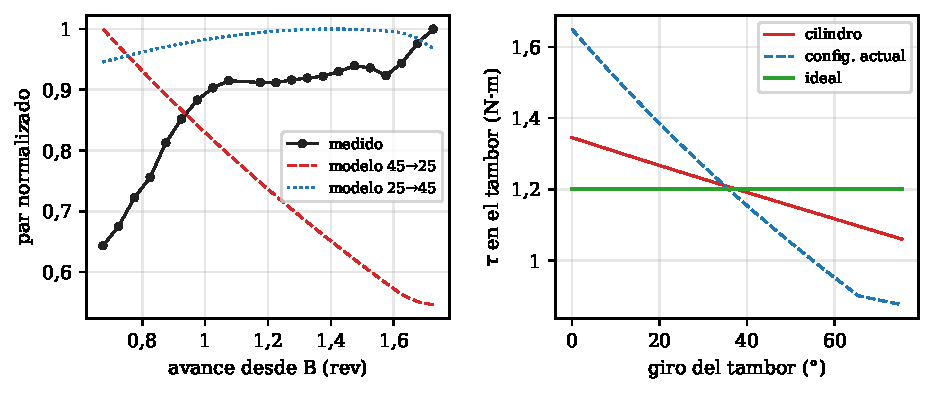
\includegraphics[width=\textwidth]{n_perfiles.pdf}
\caption{Izquierda: par medido (normalizado) frente a las dos orientaciones posibles del perfil.
Derecha: par en el tambor para el cilindro equivalente, la caracola configurada y el perfil ideal.}
\label{fig:perfiles}
\end{figure}

\section{Método experimental: separación del par y radio efectivo}
\label{sec:mod-separacion}

El accionamiento entrega el par en unidades internas de escala desconocida, y el par medido incluye
las pérdidas por rozamiento. Para comparar con el modelo sin depender de esa escala se recorre el
mismo punto en los dos sentidos, a la misma velocidad. Las pérdidas se oponen siempre al
movimiento, mientras que el par gravitatorio conserva el signo:
\begin{equation}
  |\tau_{\uparrow}(p)| = \tau_g(p) + \tau_f(p), \qquad
  |\tau_{\downarrow}(p)| = \tau_g(p) - \tau_f(p),
\end{equation}
\begin{equation}
  \tau_g = \frac{|\tau_{\uparrow}| + |\tau_{\downarrow}|}{2}, \qquad
  \tau_f = \frac{|\tau_{\uparrow}| - |\tau_{\downarrow}|}{2}.
  \label{eq:separacion}
\end{equation}
El mismo promedio aplicado a la señal de la célula elimina en primera aproximación el retardo de su
filtro, que desplaza en sentidos opuestos las curvas de ida y de vuelta.

Con $\tau_g$ ya limpio de pérdidas, la ecuación~\eqref{eq:par} permite estimar el \emph{radio
efectivo}
\begin{equation}
  r_{\text{ef}}(p) \;\propto\; \frac{\tau_g(p)}{T(p)},
  \label{eq:radio-efectivo}
\end{equation}
donde $T$ se toma del modelo, que no necesita la célula de carga: sólo la geometría y la masa. En un
tambor cilíndrico $r_{\text{ef}}$ sería constante; su forma es, por tanto, una medida directa del
perfil del tambor.

\subsection{Por qué no basta con medir la fuerza}
\label{sec:mod-ambiguedad}

Podría pensarse que basta con comparar la señal de la célula con la tensión del modelo. No es así, y
esto condiciona todo el capítulo de resultados. Como la célula no está calibrada, la comparación se
hace ajustando una recta $T \approx a\,(\text{cuentas}) + b$, y el coeficiente de determinación de
ese ajuste es el cuadrado del coeficiente de correlación:
\begin{equation}
  R^2 = \rho^2 .
\end{equation}
El valor de $R^2$ \emph{no cambia si se invierte el signo de $a$}. Una geometría que prediga una
tensión creciente y otra que la prediga decreciente pueden dar exactamente el mismo $R^2$ frente a
los mismos datos, y sólo difieren en el signo de la sensibilidad de la célula, que es precisamente
lo que no se conoce. La medida de fuerza, por sí sola, no puede decidir en qué sentido trabaja el
mecanismo.

El par del accionamiento sí puede: su signo y su escala son conocidos y no dependen de ninguna
calibración pendiente. Por eso el criterio que se usa en el capítulo~\ref{chap:resultados} es
comparar $\tau_g$ con el par del modelo, y no sólo la fuerza.

\section{Limitaciones del modelo}

\begin{itemize}
  \item Los parámetros de la tabla~\ref{tab:geometria} no son cotas medidas, sino un ajuste sobre
        los ensayos; el propio capítulo~\ref{chap:resultados} muestra que no son consistentes con el
        par medido.
  \item El punto de salida del cable se desplaza con el radio de enrollamiento, lo que introduce un
        error de algunos milímetros en $L_2$ y $dx$.
  \item Se desprecian la elasticidad del cable y la masa de la barra.
  \item El rendimiento y las pérdidas se suponen iguales en los dos sentidos, en valor absoluto,
        para poder aplicar~\eqref{eq:separacion}.
  \item El modelo es estático: no describe el tramo inicial en que el cable está destensado, ni los
        transitorios de arranque e inversión.
\end{itemize}


\chapter{Requisitos y arquitectura del banco}
\label{chap:arquitectura}

\section{Requisitos}

Los requisitos salen de lo que exige el ensayo de la caracola (capítulo~\ref{chap:modelo}). El eje
debe moverse a velocidad constante y conocida en los dos sentidos, y hay que registrar
simultáneamente, con la misma base de tiempos, la posición, la tensión del cable y el par del motor.
Todo ello de forma segura y repetible.

\subsection{Requisitos funcionales}

\begin{longtable}{@{}L{0.09\textwidth}L{0.85\textwidth}@{}}
\toprule
\textbf{Id.} & \textbf{Requisito} \\
\midrule
\endhead
RF1 & Configurar y habilitar el accionamiento y gobernar su velocidad por Modbus RTU sobre RS-485. \\
RF2 & Leer la velocidad y el par del motor en cada periodo de control. \\
RF3 & Leer la tensión del cable con una célula de carga y un acondicionador digital. \\
RF4 & Detectar los finales de carrera A (arriba) y B (abajo) y detener el movimiento hacia un final activado. \\
RF5 & Ejecutar una rutina de \emph{homing} que localice A, mida el recorrido hasta B y fije el origen en un desplazamiento configurable. \\
RF6 & Ejecutar ciclos de ensayo B$\rightarrow$A$\rightarrow$B: colocarse en el extremo inferior, subir hasta A y volver a bajar, con velocidad y número de repeticiones configurables. \\
RF7 & Enviar al ordenador la telemetría de cada periodo con su marca de tiempo del dispositivo. \\
RF8 & Recibir órdenes y parámetros desde el ordenador con detección de errores. \\
RF9 & Consultar y programar la ganancia y el cero del acondicionador de la célula, sólo con el eje parado. \\
RF10 & Mostrar el estado de la máquina y los datos en tiempo real en un navegador. \\
RF11 & Grabar automáticamente cada ensayo en un fichero con datos brutos y constantes de conversión. \\
RF12 & Visualizar los ensayos grabados y compararlos con el modelo teórico. \\
RF13 & Mantener una única configuración de la geometría del mecanismo, editable desde la interfaz y compartida por el simulador y el visor de ensayos. \\
\bottomrule
\end{longtable}

\subsection{Requisitos no funcionales}

\begin{longtable}{@{}L{0.09\textwidth}L{0.85\textwidth}@{}}
\toprule
\textbf{Id.} & \textbf{Requisito} \\
\midrule
\endhead
RNF1 & \textbf{Determinismo}: periodo de control y muestreo fijo de \SI{50}{\milli\second}, con dispersión inferior a \SI{1}{\milli\second}. \\
RNF2 & \textbf{Latencia de parada}: una orden de parada, un final de carrera o el límite de fuerza deben anular la consigna en el mismo periodo en que se detectan. \\
RNF3 & \textbf{Robustez de la comunicación}: una trama corrupta no debe ejecutar ninguna orden, y el receptor debe resincronizarse solo. \\
RNF4 & \textbf{Recuperación}: la aplicación debe reconectarse sola si se desconecta o reinicia el microcontrolador. \\
RNF5 & \textbf{Reproducibilidad}: cualquier resultado debe poder recalcularse a partir de los ficheros grabados. \\
RNF6 & \textbf{Coste y disponibilidad}: componentes comerciales y herramientas libres. \\
RNF7 & \textbf{Mantenibilidad}: validación de cada subsistema con un programa de prueba propio y código documentado. \\
RNF8 & \textbf{Coherencia del modelo}: una sola implementación de la geometría para todas las páginas, para que el simulador y el análisis no puedan discrepar. \\
\bottomrule
\end{longtable}

\section{Arquitectura general}

La figura~\ref{fig:arquitectura} muestra la arquitectura, organizada en tres niveles:

\begin{enumerate}
  \item \textbf{Nivel de campo}: el servomotor paso a paso con su accionamiento, la transmisión, la
        caracola, el cable y la barra con la masa; la célula de carga intercalada en el cable y los
        dos finales de carrera.
  \item \textbf{Nivel de control}: la placa adaptadora con la Raspberry Pi Pico~2. Ejecuta el lazo
        de \SI{50}{\milli\second} y es el único elemento que actúa sobre la máquina.
  \item \textbf{Nivel de supervisión}: un ordenador con el servidor \fichero{web\_monitor.py}, que
        traduce entre el protocolo binario del puerto USB y mensajes JSON por WebSocket, graba los
        ensayos, guarda la configuración del mecanismo y sirve las tres páginas web.
\end{enumerate}

\begin{figure}[H]
\centering
\begin{tikzpicture}[
  font=\small, >=Stealth,
  blk/.style={draw, rounded corners=2pt, align=center, minimum height=9mm, minimum width=33mm, inner sep=3pt, fill=white},
  bus/.style={<->, thick},
  grp/.style={draw, dashed, rounded corners=4pt, inner sep=6pt}
]
  \node[blk] (nav) at (0,0) {Navegador\\ \scriptsize monitor · ensayos · mecanismo};
  \node[blk] (srv) at (5,0) {Servidor FastAPI\\ \scriptsize web\_monitor.py};
  \node[blk] (csv) at (10,0) {Ensayos y configuración\\ \scriptsize cycles/*.csv · mecanismo.json};
  \draw[bus] (nav) -- node[below,font=\scriptsize,align=center] {WebSocket\\HTTP} (srv);
  \draw[->,thick] (srv) -- (csv);
  \node[grp, fit=(nav)(srv)(csv), label={[font=\scriptsize\bfseries,anchor=south west]north west:Ordenador}] {};
  \node[blk] (click) at (0,-3) {Load Cell 2 Click\\ \scriptsize ZSC31014, dirección 0x28};
  \node[blk, fill=blue!6] (pico) at (5,-3) {Raspberry Pi Pico 2\\ \scriptsize firmware\_posicion\_v2};
  \node[blk] (rs) at (10,-3) {Transceptor RS-485\\ \scriptsize THVD1400};
  \node[blk] (io) at (5,-4.6) {E/S de la placa\\ \scriptsize DI1--4, AIN1--3, DO1--4};
  \draw[bus] (pico) -- node[below,font=\scriptsize] {I\textsuperscript{2}C} (click);
  \draw[bus] (pico) -- node[below,font=\scriptsize,align=center] {UART\\PIO} (rs);
  \draw[bus] (pico) -- (io);
  \node[grp, fit=(click)(pico)(rs)(io), label={[font=\scriptsize\bfseries,anchor=south west]north west:Placa adaptadora}] {};
  \draw[bus] (srv) -- node[right,font=\scriptsize,align=left] {USB CDC\\ tramas + CRC-8} (pico);
  \node[blk] (lc) at (0,-7.4) {Célula de carga\\ \scriptsize puente de galgas};
  \node[blk] (fc) at (5,-7.4) {Finales de carrera\\ \scriptsize A arriba, B abajo (NC)};
  \node[blk] (drv) at (10,-7.4) {Accionamiento\\ \scriptsize servo paso a paso};
  \node[blk] (mot) at (10,-9.0) {Motor + reducción $N$\\ \scriptsize caracola $r(\varphi)$};
  \node[blk] (mec) at (5,-9.0) {Cable, barra\\ \scriptsize y masa de 2 kg};
  \draw[->,thick] (lc) -- node[pos=0.28,right,font=\scriptsize] {señal mV/V} (click);
  \draw[->,thick] (fc) -- (io);
  \draw[bus] (drv) -- node[pos=0.28,right,font=\scriptsize] {Modbus RTU} (rs);
  \draw[->,thick] (drv) -- (mot);
  \draw[->,thick] (mot) -- (mec);
  \draw[dotted,thick] (mec.west) -| (lc.south);
  \node[grp, fit=(lc)(fc)(drv)(mot)(mec), label={[font=\scriptsize\bfseries,anchor=south west]north west:Máquina}] {};
\end{tikzpicture}
\caption{Arquitectura del banco de ensayos.}
\label{fig:arquitectura}
\end{figure}

\section{Flujo de datos y temporización}

El microcontrolador ejecuta un lazo de periodo fijo (sección~\ref{sec:fw-lazo}). En cada vuelta lee
el estado del servo y de la célula, integra la posición, procesa las órdenes recibidas, actualiza
las máquinas de estado de \emph{homing} y de ciclo, aplica las protecciones y escribe la nueva
consigna; además guarda una muestra de la vuelta en un búfer. Cada \SI{200}{\milli\second} (o antes,
si el búfer se llena) el búfer se envía en una sola trama, con una marca de tiempo por muestra. El
servidor desempaqueta las muestras, las reenvía al navegador y, si hay un ensayo en marcha, las
escribe en su fichero. Toda la cadena usa el reloj del microcontrolador, de modo que las gráficas y
los ficheros reflejan los instantes reales de medida y no los de llegada al ordenador.

La geometría del mecanismo sigue el camino contrario: se edita en la página de configuración, se
valida y se guarda en el servidor (\fichero{mecanismo.json}), y desde ahí la leen tanto el simulador
como el visor de ensayos, de modo que el modelo con el que se compara una medida es siempre el
mismo.

\section{Decisiones de diseño}

\begin{longtable}{@{}L{0.19\textwidth}L{0.21\textwidth}L{0.48\textwidth}@{}}
\caption{Decisiones de diseño y alternativas consideradas.}\label{tab:decisiones}\\
\toprule
\textbf{Aspecto} & \textbf{Elección} & \textbf{Justificación / alternativa descartada} \\
\midrule
\endfirsthead
\toprule
\textbf{Aspecto} & \textbf{Elección} & \textbf{Justificación / alternativa descartada} \\
\midrule
\endhead
Microcontrolador & Raspberry Pi Pico 2 & Sustituye al ESP32-S3 inicial. La placa se diseñó para el módulo Pico, y su PIO permite una UART en los pines que imponía el trazado. \\
Modo del servo & Velocidad & Los primeros firmwares usaban el modo par con un regulador sobre la célula. El ensayo cuasiestático y el método de separación del par (sección~\ref{sec:mod-separacion}) exigen velocidad constante e igual en ambos sentidos. \\
Organización del firmware & Un único dueño de cada bus en el núcleo 0 & La versión de doble núcleo dedicaba el núcleo 1 a Modbus con variables compartidas. El lazo único de periodo fijo elimina las condiciones de carrera y hace predecible la temporización. \\
Origen del ciclo & Arranca en B, el extremo inferior & El ensayo tiene sentido físico desde la extensión completa del mecanismo. Como el \emph{homing} deja el eje en A, el ciclo se coloca primero en B, y ese tramo ni cuenta como repetición ni se graba. \\
Extremos del ciclo & Finales de carrera & Reconocer A y B por los finales, y no por la posición integrada, hace que el ciclo funcione esté donde esté el cero y sin depender de la escala de velocidad del accionamiento. \\
Protocolo con el PC & Binario con CRC-8 y telemetría por lotes & Un protocolo de texto ocupa más y es ambiguo de delimitar. Las tramas binarias con cabecera, longitud y CRC se resincronizan solas. \\
Posición & Integración de la velocidad del servo & No requiere cablear el codificador. Su deriva se acota con el \emph{homing} y los finales de carrera (sección~\ref{sec:fw-posicion}). \\
Células de carga & Una sola (ZSC31014) & El NAU7802 se evaluó como segunda célula y se retiró: compartían bus y el ZSC31014 no tolera transacciones ajenas entre la petición y la recogida del dato. \\
Supervisión & Aplicación web local & No requiere licencias, admite varios clientes y separa la operación en vivo del análisis. \\
Modelo del mecanismo & Una implementación única en el servidor & Cada página tenía su copia de las fórmulas y llegaron a discrepar: el monitor seguía con un cilindro mientras el visor usaba la caracola. Ahora la geometría vive en \fichero{mecanismo.json} y las fórmulas en \fichero{mecanismo.js}. \\
Datos grabados & Cuentas brutas + constantes en la cabecera & Permite recalibrar un ensayo sin repetirlo, que es justo lo que ha hecho falta. \\
\bottomrule
\end{longtable}

\section{Seguridad}
\label{sec:arq-seguridad}

El prototipo mueve una masa pequeña a baja velocidad, pero el sistema incluye varias medidas de
seguridad, todas implementadas en el firmware:

\begin{itemize}
  \item \textbf{Finales de carrera normalmente cerrados} conectados entre la entrada y masa, con
        \emph{pull-up} interna. En reposo la entrada lee nivel bajo, y un final pulsado o un cable
        roto dan nivel alto: la rotura de cable se interpreta como final activado (comportamiento a
        prueba de fallos).
  \item \textbf{Parada hacia el final activado}: en cada periodo se anula cualquier consigna que
        empuje hacia un final pulsado, sea cual sea el modo (manual, \emph{homing} o ciclo).
  \item \textbf{Límite de fuerza} configurable: si el valor absoluto de la célula tarada supera el
        umbral, la consigna se anula. Sólo actúa con una lectura válida reciente (menos de
        \SI{150}{\milli\second}).
  \item \textbf{Temporizadores de tramo} de \SI{30}{\second} en el \emph{homing} y en los ciclos.
  \item \textbf{Bloqueo durante la programación de la célula}, que la deja sin medida durante
        cientos de milisegundos: se rechaza si el eje no está parado y, mientras dura, se fuerza la
        consigna a cero en cada vuelta.
  \item \textbf{Orden de parada} que corta también el \emph{homing} y los ciclos, y orden de apagado
        que deshabilita el accionamiento.
\end{itemize}

Estas medidas dependen del software y del enlace Modbus. En una máquina industrial, las normas de
seguridad funcional exigirían una cadena de parada independiente del control \cite{iso13849}, por
ejemplo cableando los finales de carrera a la entrada de desconexión segura del par (STO) del
accionamiento \cite{iec61800}. Se recoge como trabajo futuro en el
capítulo~\ref{chap:conclusiones}.


\include{capitulos/hardware}

\chapter{Firmware del microcontrolador}
\label{chap:firmware}

\section{Entorno y organización}

El firmware está escrito en C++ con el entorno Arduino y el núcleo Arduino-Pico \cite{arduinopico},
que da acceso a los periféricos del RP2350 y a su SDK. Usa las bibliotecas \codigo{Wire}
(I\textsuperscript{2}C), \codigo{SerialPIO} (UART implementada con PIO) y ModbusMaster
\cite{modbusmaster}. El código final está en \fichero{firmware\_posicion\_v2/}: un fichero principal
de unas 1500 líneas y la cabecera \fichero{i2c\_bus.h} con el árbitro del bus I\textsuperscript{2}C.

El diseño sigue un principio que se repite en todo el código: \emph{cada bus tiene un único dueño y
un único punto del lazo donde se usa}. Sólo dos funciones tocan el bus RS-485
(\codigo{servoReadState} y \codigo{servoAction}) y sólo dos tocan el I\textsuperscript{2}C durante el
funcionamiento (\codigo{i2cUpdate} y \codigo{lcRequestService}). El intérprete de órdenes
(\codigo{processCommand}) nunca accede a un bus: se limita a modificar variables de estado, que el
lazo lee en el punto que corresponde. Así, la llegada de una orden no puede interrumpir una
transacción a medias.

El estado vive en dos estructuras: \codigo{ControlState ctrl} (modo, errores, parámetros, célula,
posición, \emph{homing} y ciclo) y \codigo{Servo sv} (fase del enlace, dirección, conexión,
contadores de fallos, consigna pendiente y últimas lecturas).

\section{Lazo principal}
\label{sec:fw-lazo}

El núcleo 0 ejecuta un lazo con periodo mínimo de \SI{50}{\milli\second} (\codigo{LOOP\_MS}). Cada
vuelta tiene cinco fases (código~\ref{lst:loop}).

\begin{lstlisting}[language=C++,caption={Estructura del lazo principal (simplificada).},label={lst:loop}]
void loop(){
  unsigned long now = millis();  uint32_t t0us = micros();

  // == LECTURA ==
  servoReadState();      // RS-485: velocidad y par (2 transacciones)
  lcRequestService();    // consulta/programación de la célula si se ha pedido
  i2cUpdate();           // I2C: una lectura de la célula
  positionUpdate();      // integra rpm -> posición (sin buses)

  // == LÓGICA == (sin acceso a buses)
  checkCommands();       // órdenes USB -> variables de estado
  if (ctrl.lcProgBusy)      { sv.speedCmd = 0; ctrl.cycPhase = CYC_IDLE; }
  else if (homing en curso)   homingUpdate();
  else                      { homingUpdate(); cycleUpdate(); }
  // protecciones: límite de fuerza y finales de carrera anulan la consigna
  // derivación del estado de la aplicación para la telemetría

  // == ACTUACIÓN ==
  servoAction();         // RS-485: máquina de estados del servo y escritura de consigna

  // == REGISTRO ==
  recordSample(now, micros() - t0us);
  if (sampleCount >= MAX_SAMPLES || now - ctrl.lastTelemetryTime >= 200)
    telemetryFlush();    // + tramas de homing y de ciclo si están activos

  // == RITMO ==
  unsigned long dt = millis() - now;
  if (dt < LOOP_MS) delay(LOOP_MS - dt);
}
\end{lstlisting}

Este orden tiene consecuencias deliberadas:
\begin{itemize}
  \item Las protecciones se evalúan \emph{después} de la lógica y \emph{antes} de la escritura:
        ninguna consigna generada por el \emph{homing}, el ciclo o una orden manual llega al
        accionamiento sin pasar por ellas.
  \item Una orden recibida se aplica en la misma vuelta, porque la escritura de la consigna es
        posterior a la lectura de órdenes.
  \item El tiempo de trabajo (\codigo{work\_us}) se mide antes del retardo de ritmo y viaja con cada
        muestra. Es la base de la caracterización temporal de la
        sección~\ref{sec:res-temporizacion}.
  \item El retardo final hace que el periodo no dependa de la duración del trabajo mientras ésta no
        supere \SI{50}{\milli\second}.
\end{itemize}

El núcleo 1 no se usa (\codigo{loop1()} sólo espera). La evolución desde la versión de doble núcleo
se explica en la sección~\ref{sec:prob-uart}.

\section{Máquina de estados del servo}

La figura~\ref{fig:fsm-servo} muestra la máquina de estados del enlace con el accionamiento, que
ejecuta \codigo{servoAction}.

\begin{figure}[H]
\centering
\begin{tikzpicture}[font=\small,>=Stealth,node distance=18mm and 26mm,
  st/.style={draw,rounded rectangle,minimum width=24mm,minimum height=8mm,fill=blue!5}]
  \node[st] (idle) {SV\_IDLE};
  \node[st,right=of idle] (cfg) {SV\_CONFIGURING};
  \node[st,right=of cfg] (run) {SV\_RUNNING};
  \node[st,below=24mm of cfg] (fault) {SV\_FAULT};
  \draw[->] (idle) -- node[above,font=\scriptsize]{INIT} (cfg);
  \draw[->] (cfg) -- node[above,font=\scriptsize]{configuración OK} (run);
  \draw[->] ([xshift=6mm]cfg.south) -- node[right,font=\scriptsize]{3 fallos} ([xshift=6mm]fault.north);
  \draw[->] (cfg.north) to[bend right=35] node[above,font=\scriptsize]{STOP} (idle.north);
  \draw[->] (run.south) |- node[pos=0.25,right,font=\scriptsize]{SHUTDOWN} ([yshift=-9mm]idle.south) -- (idle.south);
  \draw[->] ([xshift=-6mm]fault.north) -- node[left,font=\scriptsize]{INIT} ([xshift=-6mm]cfg.south);
  \draw[->] (run) edge[loop above] node[above,font=\scriptsize]{escritura de consigna cada 50 ms} (run);
\end{tikzpicture}
\caption{Máquina de estados del enlace con el accionamiento.}
\label{fig:fsm-servo}
\end{figure}

En \codigo{SV\_CONFIGURING} se ejecuta la secuencia de configuración del
capítulo~\ref{chap:comunicaciones}. En \codigo{SV\_RUNNING} cada vuelta escribe la consigna: un
fallo marca el servo como desconectado y pone a cero las lecturas, pero no provoca un nuevo escaneo
del bus, que es bloqueante y lento (hasta un segundo por dirección vacía). El escaneo sólo se hace
bajo demanda con la orden SCAN.

La orden INIT, además de reiniciar la posición, invalida el recorrido A$\rightarrow$B medido: poner
el cero donde esté el eje deja sin sentido la referencia anterior, y sin esa invalidación el ciclo
podría creer que A es el punto actual.

\section{Lectura de la célula de carga}

El ZSC31014 trabaja en modo de conversión continua: convierte a su propio ritmo, fijado por la
palabra ZMDI\_Config1, de \num{0.5} a \SI{125}{\milli\second} según el reloj y la tasa elegidos
\cite{zsc31014}, y guarda el último resultado. Una lectura no dispara una conversión: devuelve el
último dato con dos bits de estado que indican si es nuevo o si ya se había leído.

Por ello, \codigo{loadCellUpdate} hace \emph{una sola lectura de dos bytes por vuelta}:
\begin{enumerate}
  \item Pide el bus al árbitro. Si está ocupado, pierde el turno y lo intenta en la vuelta
        siguiente.
  \item Lee 14 bits de dato y 2 de estado. Si el estado es ``dato válido'', lo introduce en una
        media móvil de 8 posiciones y calcula la lectura tarada
        \codigo{baseRead = media $-$ zeroOffset}.
  \item Si pasan más de \SI{150}{\milli\second} sin un dato válido, marca la célula como no válida y
        el límite de fuerza deja de actuar, en lugar de hacerlo con un dato viejo.
\end{enumerate}

\subsection{Árbitro del bus I\textsuperscript{2}C}

La cabecera \fichero{i2c\_bus.h} implementa un árbitro mínimo: una variable con el dueño actual
(\codigo{I2C\_FREE}, \codigo{I2C\_LC1}, \codigo{I2C\_LC2} o \codigo{I2C\_CFG}) y dos funciones,
\codigo{i2cAcquire} e \codigo{i2cRelease}. La reserva se deniega si el bus tiene otro dueño o si se
pide desde el núcleo 1, y cada denegación se cuenta para el diagnóstico. El árbitro nació al
compartir el bus con el NAU7802 (sección~\ref{sec:prob-nau}) y se conserva para reservar el bus en
exclusiva durante la programación de la EEPROM. Nadie espera con el bus ocupado, así que el árbitro
no puede bloquear el lazo.

\section{Posición integrada}
\label{sec:fw-posicion}

La posición del eje del motor se obtiene integrando la velocidad que devuelve el accionamiento:
\begin{equation}
  p_k = p_{k-1} + \frac{n_k\,\Delta t_k}{60000}, \qquad [p]=\text{rev},\ [n]=\text{rpm},\ [\Delta t]=\text{ms}.
\end{equation}
Es una integración rectangular con la última velocidad leída y el intervalo real medido con
\codigo{millis()}. Hay tres aspectos que tener en cuenta:
\begin{itemize}
  \item \textbf{Rebase tras un hueco.} Si el lazo se detiene, por ejemplo durante la programación de
        la célula, la siguiente vuelta vería un $\Delta t$ de casi un segundo y lo multiplicaría por
        la última velocidad, inventando un desplazamiento que no ha ocurrido. Por eso se anula la
        base de tiempo (\codigo{lastPosTime = 0}) tras INIT, al iniciar el \emph{homing} y tras
        cualquier operación bloqueante.
  \item \textbf{Resolución.} El registro de velocidad tiene resolución de \SI{1}{rpm}: si el
        accionamiento redondea, el error es de media nula; si trunca, a \SI{30}{rpm} introduciría un
        sesgo de hasta el \SI{3}{\percent}.
  \item \textbf{Acotación.} La deriva no se acumula entre ensayos, porque el ciclo reconoce sus
        extremos por los finales de carrera y no por la posición integrada.
\end{itemize}

Esta última decisión es la que hace que el banco siga siendo utilizable pese a la incertidumbre de
la posición: el recorrido del ensayo queda definido por dos contactos físicos, y la posición
integrada sólo sirve como eje de referencia dentro del ensayo.

\section{\emph{Homing}}

La rutina de \emph{homing} (figura~\ref{fig:homing}) establece un origen repetible y mide el
recorrido disponible:
\begin{enumerate}
  \item \textbf{Buscar A}: avanza hacia A (arriba) a la velocidad de \emph{homing} hasta que se
        activa el final A, y fija ahí $p=0$.
  \item \textbf{Buscar B}: avanza hacia B (abajo) hasta el final B y guarda el recorrido $p_B$.
  \item \textbf{Ir al origen}: se mueve hasta el desplazamiento configurado, acotado a $[0, p_B]$,
        con tolerancia de $\pm\SI{0.02}{rev}$.
  \item Fija ese punto como nuevo origen ($p=0$) y sigue informando del resultado durante
        \SI{1.5}{\second} para que la interfaz lo muestre.
\end{enumerate}
Cualquier tramo que dure más de \SI{30}{\second}, o la pérdida del servo, aborta con fallo. Durante
el \emph{homing} se ignoran las órdenes de movimiento manual.

\begin{figure}[H]
\centering
\begin{tikzpicture}[font=\small,>=Stealth,
  st/.style={draw,rounded rectangle,minimum width=22mm,minimum height=8mm,fill=green!5}]
  \node[st] (i) at (0,0) {IDLE};
  \node[st] (a) at (3.6,0) {SEEK\_A};
  \node[st] (b) at (7.6,0) {SEEK\_B};
  \node[st] (g) at (7.6,-2) {GOTO};
  \node[st] (d) at (3.6,-2) {DONE};
  \node[st,fill=red!8] (f) at (3.6,2) {FAIL};
  \draw[->] (i) -- node[above,font=\scriptsize]{HOME} (a);
  \draw[->] (a) -- node[above,font=\scriptsize]{FC A: $p\!=\!0$} (b);
  \draw[->] (b) -- node[right,font=\scriptsize]{FC B: $p_B\!=\!p$} (g);
  \draw[->] (g) -- node[above,font=\scriptsize]{$|e|\le 0{,}02$: $p\!=\!0$} (d);
  \draw[->,dashed] (d) -| node[pos=0.25,below,font=\scriptsize]{tras 1,5 s} (i);
  \draw[->,dashed] (f) -| node[pos=0.25,above,font=\scriptsize]{tras 1,5 s} (i);
  \draw[->,red!70!black] (a) -- node[right,font=\scriptsize,align=left]{timeout (30 s) o servo perdido\\ en cualquier fase activa} (f);
  \draw[->,red!70!black] (b) |- (f);
\end{tikzpicture}
\caption{Máquina de estados del \emph{homing}.}
\label{fig:homing}
\end{figure}

\section{Ciclo de ensayo B$\rightarrow$A$\rightarrow$B}
\label{sec:fw-ciclo}

El ensayo tiene sentido físico empezando por el extremo inferior, con el mecanismo en extensión
completa y la masa en su punto más bajo. Como el \emph{homing} deja el eje en A, el ciclo se
organiza en tres fases (figura~\ref{fig:ciclo}):

\begin{description}[style=nextline,leftmargin=1.5em]
  \item[\codigo{CYC\_POS\_B} --- colocación] Baja hasta B. Este tramo no cuenta como repetición y el
        servidor no lo graba: el ensayo empieza cuando el eje ya está en B. Al llegar se guarda
        \codigo{cycPosB}, la posición integrada en ese punto, que será el origen de medida del
        ensayo.
  \item[\codigo{CYC\_TO\_A} --- ida] Sube hasta A. Es el tramo cargado del ensayo.
  \item[\codigo{CYC\_TO\_B} --- vuelta] Baja de nuevo hasta B y cierra la repetición; si quedan
        repeticiones, se vuelve a \codigo{CYC\_TO\_A}.
\end{description}

Por convenio, la consigna negativa lleva el eje hacia A (arriba) y la positiva hacia B (abajo).

\begin{figure}[H]
\centering
\begin{tikzpicture}[font=\small,>=Stealth,
  st/.style={draw,rounded rectangle,minimum width=26mm,minimum height=8mm,fill=blue!5}]
  \node[st] (i) at (0,0) {CYC\_IDLE};
  \node[st] (p) at (4.2,0) {CYC\_POS\_B};
  \node[st] (a) at (8.6,0) {CYC\_TO\_A};
  \node[st] (b) at (8.6,-2) {CYC\_TO\_B};
  \node[st] (d) at (4.2,-2) {CYC\_DONE};
  \node[st,fill=red!8] (f) at (0,-2) {CYC\_FAIL};
  \draw[->] (i) -- node[above,font=\scriptsize]{CYCLE\_START} (p);
  \draw[->] (p) -- node[above,font=\scriptsize,align=center]{FC B\\ $p_B$ fijado} (a);
  \draw[->] (a) -- node[right,font=\scriptsize]{FC A} (b);
  \draw[->] (b) -- node[above,font=\scriptsize,align=center]{FC B: repetición\\ completada} (d);
  \draw[->] (b.north east) to[bend right=55] node[right,font=\scriptsize,align=left]{quedan\\ repeticiones} (a.south east);
  \draw[->,red!70!black] (d) -- node[above,font=\scriptsize]{timeout / servo} (f);
\end{tikzpicture}
\caption{Máquina de estados del ciclo de ensayo.}
\label{fig:ciclo}
\end{figure}

Los extremos se reconocen por los \emph{finales de carrera}, no por la posición integrada. Así el
ciclo funciona esté el cero donde esté ---el \emph{homing} puede haberlo dejado en A, en B o en
medio--- y sin depender de que la escala de velocidad del accionamiento sea exacta, que es de donde
sale la posición. Si se pide un recorrido parcial, la distancia se mide \emph{desde B}:

\begin{lstlisting}[language=C++,caption={Reconocimiento de los extremos del ciclo.},label={lst:ciclo}]
static bool cycleAtB(bool limB){            // B: el final de abajo
  if(ctrl.cycToLimitB) return limB;
  return limB || (ctrl.posRev >= ctrl.cycPosB - HOMING_TOL_REV);
}
static bool cycleAtA(bool limA){            // A: el final de arriba, o la distancia pedida
  if(ctrl.cycToLimitB) return limA;
  return limA || ((ctrl.cycPosB - ctrl.posRev) >= (ctrl.cycTargetRev - HOMING_TOL_REV));
}
\end{lstlisting}

El ciclo sólo se acepta con el servo habilitado, sin \emph{homing} en curso y sin programación de la
célula. Los temporizadores y la pérdida del servo lo abortan, y los finales de carrera y el límite
de fuerza siguen actuando en el lazo como red de seguridad. La prioridad es: programación de la
célula $>$ \emph{homing} $>$ ciclo $>$ movimiento manual.

\section{Configuración del acondicionador de la célula}

La consulta y la programación de la EEPROM del ZSC31014 son las operaciones más delicadas del
firmware. Por las restricciones que se analizan en la sección~\ref{sec:prob-zsc}, obligan a
reiniciar el chip y dejan la célula sin medida durante cientos de milisegundos. Se ejecutan así:

\begin{enumerate}
  \item \codigo{processCommand} sólo \emph{anota} la petición y un plazo de \SI{1}{\second}.
  \item En su punto fijo del lazo, \codigo{lcRequestService} comprueba que el eje está en reposo:
        estado IDLE o STOPPED, consigna nula y sin \emph{homing}. Si no lo está, responde
        ``rechazado''.
  \item Reserva el bus en exclusiva (\codigo{I2C\_CFG}). Si no lo consigue antes del plazo, responde
        ``bus ocupado''.
  \item Pone la consigna a cero, pasa al estado PROGRAMMING y envía la telemetría pendiente para que
        la interfaz vea el silencio que viene.
  \item Ejecuta la consulta o la programación, devuelve el bus a \SI{400}{\kilo\hertz}, libera el
        árbitro, reinicializa la célula, anula la base de la integración de posición y responde con
        el paquete \codigo{0x04}.
\end{enumerate}

\subsection{Escritura verificada}

\codigo{loadCellProgram} aplica dos reglas de la hoja de datos \cite{zsc31014}: la palabra
ZMDI\_Config1 sólo se carga tras un ciclo de alimentación, y la firma MISR de la EEPROM (palabra
\codigo{0x12}) se regenera al salir del modo comando con Start\_NOM si hubo escrituras. La función
hace dos pasadas:

\begin{enumerate}
  \item \textbf{Primera pasada}: entra en modo comando, lee B\_Config (\codigo{0x0F}) y
        ZMDI\_Config1 (\codigo{0x01}) y calcula las palabras deseadas. Si coinciden con las
        actuales, termina sin escribir, porque la EEPROM admite 100.000 ciclos de escritura. Si no,
        escribe las que cambian, espera \SI{20}{\milli\second} por escritura (típico
        \SI{15}{\milli\second}, peor caso \SI{17.3}{\milli\second}), envía Start\_NOM y espera
        \SI{150}{\milli\second} antes de cortar la alimentación.
  \item \textbf{Segunda pasada}: desde un reinicio limpio, vuelve a leer ambas palabras. Si
        coinciden con lo pedido, el resultado es ``grabado y verificado''; si no, ``fallo''.
\end{enumerate}

Las palabras deseadas se construyen a partir de las actuales, protegiendo los bits que la interfaz
no debe tocar: en B\_Config se conservan los reservados [15:13]; en ZMDI\_Config1 se conservan
[15:9] (signos de las correcciones de segundo orden y de temperatura, calibrados en fábrica) y se
fuerzan el interfaz I\textsuperscript{2}C (bit 4 = 0) y el campo reservado [2:0] = 001.

\subsection{Mantenimiento del reinicio para medida}

La orden LC\_HOLD deja la célula sin alimentación durante \SI{8}{\second}, con las líneas del bus en
el estado elegido, para medir con un polímetro la tensión de la placa Click. A diferencia de la
programación, esta espera \emph{no} bloquea: el lazo sigue girando, leyendo el servo, vigilando los
finales de carrera y enviando telemetría, y en cada vuelta sólo comprueba si ha vencido el plazo.
Mientras dura se fuerza la consigna a cero en cada vuelta: alguien tiene las manos dentro de la
máquina, y una orden de movimiento que llegue por USB no debe poder arrancar el eje.

\section{Evolución del firmware}

\begin{longtable}{@{}L{0.27\textwidth}L{0.12\textwidth}L{0.49\textwidth}@{}}
\caption{Versiones del firmware conservadas en el repositorio.}\label{tab:versiones-fw}\\
\toprule
Versión & Placa & Características \\
\midrule
\endfirsthead
\toprule
Versión & Placa & Características \\
\midrule
\endhead
\fichero{old/speedtorque\_mode} & XIAO ESP32-S3 & Escaneo Modbus y selección de modo par o velocidad. \\
\fichero{firmware} & XIAO ESP32-S3 & Protocolo binario v2, parámetros del accionamiento y regulador de fuerza en modo par con zona muerta, umbral y ganancia sobre la célula filtrada. \\
\fichero{firmwarerasp} & Pico 2 & Migración con SerialPIO. Doble núcleo: el núcleo 1 escribe la consigna y lee la supervisión Modbus, comunicado con el núcleo 0 por variables \codigo{volatile}. \\
\fichero{firmware\_posicion} & Pico 2 & Modo velocidad sin lazo de fuerza, integración de posición, telemetría por lotes y diseño de dueño único en el núcleo 0. \\
\fichero{firmware\_posicion\_v2} & Pico 2 & Versión final: \emph{homing}, ciclo B$\rightarrow$A$\rightarrow$B con extremos por finales de carrera, programación verificada de la EEPROM, árbitro I\textsuperscript{2}C y diagnóstico en la telemetría. \\
\bottomrule
\end{longtable}


\chapter{Comunicaciones}
\label{chap:comunicaciones}

El sistema usa cuatro enlaces (tabla~\ref{tab:enlaces}). Este capítulo describe el protocolo binario
propio entre el microcontrolador y el ordenador, el uso de Modbus RTU con el accionamiento y la
interfaz entre el servidor y el navegador. La especificación byte a byte está en el
anexo~\ref{anx:protocolo}.

\begin{table}[H]
\centering
\caption{Enlaces de comunicación del sistema.}
\label{tab:enlaces}
\small
\begin{tabularx}{\textwidth}{@{}lL{0.27\textwidth}XX@{}}
\toprule
Enlace & Extremos & Capa física & Protocolo \\
\midrule
USB & PC $\leftrightarrow$ Pico & USB CDC (puerto serie virtual) & Binario propio + CRC-8 \\
RS-485 & Pico $\leftrightarrow$ accionamiento & UART PIO, 115200 8N1 & Modbus RTU \\
I\textsuperscript{2}C1 & Pico $\leftrightarrow$ ZSC31014 & \SI{400}{\kilo\hertz} (\SI{100}{\kilo\hertz} en modo comando) & Propio del chip \\
Red local & Navegador $\leftrightarrow$ servidor & TCP, puerto 8080 & HTTP + WebSocket (JSON) \\
\bottomrule
\end{tabularx}
\end{table}

\section{Protocolo binario entre el microcontrolador y el ordenador}

\subsection{Formato de trama}

Todas las tramas, en ambos sentidos, tienen el mismo formato (figura~\ref{fig:trama}): dos bytes de
sincronía \codigo{0xAA 0x55}, un byte de longitud, la carga útil y un CRC-8 calculado sobre la carga
útil. El primer byte de la carga útil identifica el tipo de paquete o la orden. Los enteros
multibyte van en orden \emph{little-endian}.

\begin{figure}[H]
\centering
\begin{bytefield}[bitwidth=2.4em]{12}
  \bitbox{2}{\small 0xAA} & \bitbox{2}{\small 0x55} & \bitbox{2}{\small LEN} &
  \bitbox{1}{\small ID} & \bitbox{3}{\small datos (LEN$-$1)} & \bitbox{2}{\small CRC-8}
\end{bytefield}
\caption{Formato común de trama. El CRC-8 cubre los LEN bytes de la carga útil (ID + datos).}
\label{fig:trama}
\end{figure}

El CRC usa el polinomio $x^8+x^2+x+1$ (\codigo{0x07}), valor inicial \codigo{0x00}, sin reflexión ni
XOR final (la variante conocida como CRC-8/SMBUS). Se implementa bit a bit en el firmware y en
Python con el mismo algoritmo. Para tramas cortas como éstas detecta todos los errores de uno y dos
bits y todas las ráfagas de hasta 8 bits.

\subsection{Recepción y resincronización}

El firmware decodifica las órdenes con una máquina de cuatro estados (\codigo{RX\_SYNC0},
\codigo{RX\_SYNC1}, \codigo{RX\_LEN}, \codigo{RX\_PAYLOAD}). Una longitud nula o mayor de 60 devuelve
el decodificador a la búsqueda de sincronía, y una trama con CRC incorrecto se descarta sin
ejecutarse. Si se pierden bytes, el receptor vuelve a encontrar el patrón \codigo{AA 55} en la
siguiente trama. El servidor hace lo mismo con la telemetría, con un tiempo de espera de
\SI{100}{\milli\second} por lectura.

Para depurar desde un terminal, el firmware acepta también órdenes de una letra (\codigo{i},
\codigo{a}, \codigo{b}, \codigo{x}, \codigo{h}, \codigo{q}), pero \emph{sólo} cuando el decodificador
está esperando el primer byte de sincronía. Antes se comprobaban en cualquier estado, y eso
provocaba un error difícil de ver: la orden de programar la célula con ganancia 7 y cero 8 genera la
trama \codigo{AA 55 03 09 07 08 69}, cuyo CRC \codigo{0x69} coincide con el carácter \codigo{i}. El
atajo se comía el último byte, la orden se perdía y además se reinicializaba el servo. Con ganancia
6 el CRC vale \codigo{0x7C} y la misma orden funcionaba. Ambos valores se han comprobado con la
implementación del CRC.

\subsection{Paquetes del microcontrolador al ordenador}

\begin{table}[H]
\centering
\caption{Paquetes de telemetría y estado.}
\label{tab:paquetes}
\begin{tabular}{@{}clll@{}}
\toprule
ID & Nombre & Tamaño de carga útil & Cuándo se envía \\
\midrule
\codigo{0x02} & Telemetría por lotes & $14 + 14n$ B, $n\le 8$ & cada \SI{200}{\milli\second} o con 8 muestras \\
\codigo{0x03} & Estado de \emph{homing} & 11 B & junto al lote, mientras hay \emph{homing} \\
\codigo{0x04} & Resultado de la célula & 13 B & una vez por consulta o programación \\
\codigo{0x05} & Estado del ciclo & 18 B & junto al lote, mientras hay ciclo \\
\bottomrule
\end{tabular}
\end{table}

\paragraph{Telemetría por lotes.} Cada vuelta del lazo añade al búfer una muestra de 14 bytes:
desfase en milisegundos respecto al instante base del lote, velocidad, par, consigna, fuerza tarada,
estado de los finales de carrera, estado de la máquina y tiempo de trabajo de la vuelta. Los datos
comunes (instante base de 32 bits, lectura bruta de la célula y su estado, indicadores, código de
error, dirección del servo y códigos de resultado de las dos lecturas Modbus) viajan una sola vez en
una cabecera de 14 bytes.

Agrupar las muestras reduce las escrituras por USB a cinco por segundo sin perder resolución
temporal, porque cada muestra conserva su instante exacto. Con el lazo de \SI{50}{\milli\second} cada
lote lleva típicamente cuatro muestras: 70 bytes de carga útil, 74 de trama y unos
\SI{370}{\byte\per\second}, muy por debajo de la capacidad del enlace. El precio es un retardo de
visualización de hasta \SI{200}{\milli\second} y que la lectura bruta de la célula sólo se refresque
una vez por lote (sección~\ref{sec:res-limitaciones}).

\paragraph{Estado del ciclo.} El paquete \codigo{0x05} creció de 14 a 18 bytes al reorganizar el
ciclo: además de la fase, las repeticiones y la posición, transporta \codigo{cycPosB}, la posición
en la que ha quedado fijado el punto B. Sin ese dato no se puede saber desde fuera contra qué está
midiendo el ciclo un recorrido parcial. Las fases son ahora seis: reposo, colocándose en B, hacia A,
volviendo a B, completado y abortado.

Para que un firmware y un servidor desparejados no se queden mudos, el servidor acepta también la
trama de 14 bytes de la versión anterior y asume \codigo{cycPosB = 0}. Esa compatibilidad se añadió
precisamente porque un desajuste de versiones despistó durante la depuración del ciclo: el firmware
enviaba una trama que el servidor rechazaba entera, y la interfaz no mostraba ninguna fase.

\paragraph{Modelo pregunta-respuesta de la célula.} Cada orden de consulta, programación o
mantenimiento de la célula produce exactamente un paquete \codigo{0x04}, también cuando se rechaza.
El paquete incluye el código de la orden a la que responde, para que la interfaz nunca se quede
esperando, y lleva información de diagnóstico: el primer byte que devolvió el chip, si el pin de
reinicio corta de verdad la alimentación y en qué intento del barrido de retardos se consiguió
entrar en modo comando (sección~\ref{sec:prob-zsc}).

\subsection{Órdenes del ordenador al microcontrolador}

\begin{longtable}{@{}clL{0.30\textwidth}L{0.33\textwidth}@{}}
\caption{Órdenes aceptadas por el firmware.}\label{tab:ordenes}\\
\toprule
Código & Nombre & Datos & Efecto \\
\midrule
\endfirsthead
\toprule
Código & Nombre & Datos & Efecto \\
\midrule
\endhead
\codigo{0x01} & INIT & [dirección Modbus] opcional & Reinicia la posición, invalida el recorrido medido y configura y habilita el servo. \\
\codigo{0x02} & STOP & -- & Consigna a cero; aborta \emph{homing} y ciclo. \\
\codigo{0x03} & SET\_PARAM & id (1 B), valor int16 & Modifica un parámetro (tabla~\ref{tab:parametros}). \\
\codigo{0x04} & MOVE\_A & -- & Movimiento manual hacia A (arriba). \\
\codigo{0x05} & MOVE\_B & -- & Movimiento manual hacia B (abajo). \\
\codigo{0x06} & SHUTDOWN & -- & Deshabilita el accionamiento. \\
\codigo{0x07} & SCAN & -- & Búsqueda bloqueante del esclavo (1--247). \\
\codigo{0x08} & HOME & -- & Inicia el \emph{homing}. \\
\codigo{0x09} & LC\_PROGRAM & B\_Config, ZMDI\_Config1 (uint16) & Graba la configuración de la célula (sólo parado). \\
\codigo{0x0A} & LC\_QUERY & -- & Lee la configuración de la célula (sólo parado). \\
\codigo{0x0B} & LC\_HOLD & modo de aparcado (1 B) & Mantiene la célula sin tensión \SI{8}{\second} para medirla. \\
\codigo{0x0C} & CYCLE\_START & modo, recorrido (centi-rev), velocidad, repeticiones & Inicia el ciclo B$\rightarrow$A$\rightarrow$B, empezando por la colocación en B. \\
\codigo{0x0D} & CYCLE\_STOP & -- & Detiene el ciclo donde esté. \\
\bottomrule
\end{longtable}

\begin{table}[H]
\centering
\caption{Parámetros configurables con SET\_PARAM.}
\label{tab:parametros}
\begin{tabular}{@{}cllr@{}}
\toprule
Id & Parámetro & Unidad & Defecto \\
\midrule
1 & Velocidad de movimiento manual & rpm & 10 \\
2 & Límite de fuerza (0 = desactivado) & cuentas & 0 \\
3 & Tara de la célula & cuentas & 8210 \\
4 & Aceleración (C03.22) & u. del accionamiento & 5 \\
5 & Deceleración (C03.24) & u. del accionamiento & 5 \\
6 & Rigidez (C00.05) & nivel & 10 \\
7 & Calibración de fuerza (sólo informativa) & cuentas/N & 0 \\
8 & Desplazamiento del origen tras el \emph{homing} & centi-rev & 0 \\
9 & Velocidad de \emph{homing} & rpm & 30 \\
\bottomrule
\end{tabular}
\end{table}

\section{Modbus RTU con el accionamiento}

\subsection{Registros utilizados}

El firmware sólo usa las funciones 0x03 y 0x06 sobre un conjunto reducido de registros
(anexo~\ref{anx:modbus}). Los parámetros del accionamiento se nombran \codigo{Cgg.ii}, y todas las
direcciones cumplen la regla
\begin{equation}
  \text{dirección} = 256\cdot gg + \text{0x}ii,
\end{equation}
es decir, el índice se interpreta en hexadecimal. Por ejemplo, C04.11 (habilitación) es
$1024 + 17 = 1041$ y C03.22 (aceleración) es $768 + 34 = 802$. Las magnitudes de supervisión están en
el grupo \codigo{0x40}: velocidad en 16385 (\codigo{0x4001}) y par en 16387 (\codigo{0x4003}). Tener
esta regla evita errores al añadir registros a partir del manual.

\subsection{Secuencia de configuración}

Al recibir INIT, el firmware configura el accionamiento así: deshabilitar (C04.11 = 0), seleccionar
el modo velocidad (C00.00 = 1), poner la consigna a cero (C03.21 = 0), escribir la rigidez y las
rampas, configurar la resistencia de frenado externa (C00.10 a C00.13) y habilitar (C04.11 = 1). Si
una escritura esencial falla se reintenta la secuencia completa, y tras tres fallos el sistema pasa
a estado de error. Entre escrituras se deja un silencio de \SI{700}{\micro\second}.

\subsection{Transacciones por periodo}

En régimen normal, cada vuelta del lazo realiza tres transacciones: lectura de la velocidad, lectura
del par y escritura de la consigna. Escribir la consigna en cada vuelta, aunque no cambie, sirve
además de supervisión del enlace: si la escritura falla, se marca el servo como desconectado.

A 115200 baudios con formato 8N1, cada byte ocupa \SI{86.8}{\micro\second}. Las tres transacciones
suman 46 bytes, unos \SI{4.0}{\milli\second} de línea. A eso se añaden \SI{0.6}{\milli\second} de
retardos de conmutación del transceptor y \SI{0.7}{\milli\second} de silencio entre las dos lecturas.
El tiempo de trabajo medido del lazo es \SI{10.97}{\milli\second}
(sección~\ref{sec:res-temporizacion}); la diferencia, unos \SI{5.7}{\milli\second}, corresponde
principalmente al tiempo de respuesta del accionamiento, aproximadamente \SI{1.9}{\milli\second} por
transacción.

La guía de implementación de Modbus serie recomienda, por encima de 19200 baudios, silencios fijos
de \SI{1.75}{\milli\second} entre tramas \cite{modbusserial}. El firmware usa
\SI{700}{\micro\second} y el accionamiento lo acepta sin errores, pero con otros esclavos convendría
respetar el valor recomendado.

\section{Interfaz entre el servidor y el navegador}

\subsection{WebSocket}

El servidor mantiene una conexión WebSocket en \codigo{/ws} con cada navegador. En sentido servidor
$\rightarrow$ navegador envía objetos JSON de cinco tipos:
\begin{itemize}
  \item \textbf{muestra de telemetría} (sin campo \codigo{type}): una por muestra del lote, con los
        valores brutos, los nombres de estado y error ya traducidos, la posición integrada, los
        finales de carrera, la frecuencia de muestreo medida y el estado del \emph{homing};
  \item \codigo{home}: fase del \emph{homing}, posición y recorrido medido;
  \item \codigo{cycle}: fase, repeticiones hechas y pedidas, posición, recorrido pedido, posición de
        B y fichero en grabación;
  \item \codigo{lc\_config}: resultado de la consulta o programación de la célula;
  \item \codigo{cmd\_ack}: confirmación de \emph{toda} orden recibida, con indicación de éxito y un
        texto explicativo. Sin ella, una orden que no llegaba al puerto era indistinguible de una
        que sí se había ejecutado.
\end{itemize}

En sentido navegador $\rightarrow$ servidor, las órdenes son objetos
\codigo{\{"cmd": nombre,} \codigo{...parámetros\}}. El servidor las valida, limita los parámetros a
rangos seguros (por ejemplo, velocidad del ciclo entre 0 y \SI{300}{rpm}), construye la trama
binaria y la escribe en el puerto.

\subsection{Servicios HTTP}

\begin{table}[H]
\centering
\caption{Servicios HTTP del servidor.}
\label{tab:http}
\begin{tabular}{@{}lll@{}}
\toprule
Método & Ruta & Función \\
\midrule
GET & \codigo{/} & Monitor en tiempo real \\
GET & \codigo{/ensayos} & Visor de ensayos grabados \\
GET & \codigo{/sim} & Configuración del mecanismo y simulador \\
GET & \codigo{/api/mecanismo} & Geometría actual (JSON) \\
PUT & \codigo{/api/mecanismo} & Guarda la geometría, validada contra rangos \\
GET & \codigo{/cycles} & Lista de los 50 ensayos más recientes (JSON) \\
GET & \codigo{/cycles/\{nombre\}} & Descarga de un ensayo (CSV) \\
DELETE & \codigo{/cycles/\{nombre\}} & Borrado de un ensayo (rechazado si se está grabando) \\
GET & \codigo{/mecanismo.js}, \codigo{/tema.css}, \codigo{/tema.js}, \codigo{/nav.js} & Recursos comunes a las tres páginas \\
\multicolumn{2}{@{}l}{\codigo{/fui} (montaje estático)} & Kit de interfaz (hoja de estilo y tipografías) \\
\bottomrule
\end{tabular}
\end{table}

Las rutas con nombre de fichero reducen el parámetro a su último componente antes de usarlo, de modo
que una petición con \codigo{../} no puede leer ni borrar ficheros fuera de la carpeta de ensayos.
La escritura de la geometría se valida en el servidor contra los mismos rangos que comprueba el
navegador, de forma que una petición construida a mano tampoco puede dejar una configuración
imposible.


\chapter{Software de supervisión y análisis}
\label{chap:software}

\section{Visión general}

El software del ordenador consta de un servidor en Python (\fichero{web\_monitor.py}), tres páginas
web y varias herramientas auxiliares. El servidor se ejecuta con

\begin{lstlisting}[language=bash,numbers=none]
python web_monitor.py [puerto_serie]      # http://localhost:8080
\end{lstlisting}

y detecta solo el puerto del microcontrolador si no se indica. Las tres páginas son el
\emph{monitor} en tiempo real (\codigo{/}), el \emph{visor de ensayos} (\codigo{/ensayos}) y la
\emph{configuración del mecanismo} con simulador (\codigo{/sim}), enlazadas entre sí por una barra
de teclas programables común.

\section{Servidor}

\subsection{Estructura concurrente}

El servidor combina un hilo del sistema operativo para el puerto serie con el bucle asíncrono de
FastAPI (figura~\ref{fig:servidor}).

\begin{figure}[H]
\centering
\begin{tikzpicture}[font=\small,>=Stealth,
  box/.style={draw,rounded corners=2pt,align=center,minimum height=10mm,inner sep=4pt,fill=white}]
  \node[box,minimum width=28mm] (usb) {Puerto USB\\ \scriptsize pySerial};
  \node[box,minimum width=34mm,right=10mm of usb,fill=blue!6] (hilo) {Hilo serie\\ \scriptsize decodifica · integra · graba};
  \node[box,minimum width=24mm,right=10mm of hilo] (cola) {deque\\ \scriptsize maxlen = 100};
  \node[box,minimum width=30mm,right=10mm of cola,fill=green!6] (bc) {Difusor asíncrono\\ \scriptsize FastAPI / Uvicorn};
  \node[box,minimum width=24mm,below=10mm of bc] (ws) {Navegadores\\ \scriptsize WebSocket};
  \node[box,minimum width=24mm,below=10mm of hilo] (csv) {cycles/*.csv};
  \node[box,minimum width=30mm,below=10mm of cola] (cmd) {\_handle\_command\\ \scriptsize valida · empaqueta};
  \draw[->,thick] (usb) -- (hilo);
  \draw[->,thick] (hilo) -- (cola);
  \draw[->,thick] (cola) -- (bc);
  \draw[->,thick] (bc) -- (ws);
  \draw[->,thick] (hilo) -- (csv);
  \draw[->,thick] (ws) -- (cmd);
  \draw[->,thick] (cmd.south) -- ++(0,-5mm) -| node[pos=0.25,below,font=\scriptsize]{tramas binarias} (usb.south);
\end{tikzpicture}
\caption{Estructura del servidor de supervisión.}
\label{fig:servidor}
\end{figure}

\paragraph{Hilo serie.} Abre el puerto (probando \codigo{/dev/ttyACM*}, \codigo{/dev/ttyUSB*},
\codigo{/dev/cu.usbmodem*} y \codigo{COM*}), vacía el búfer y entra en un bucle que lee tramas,
comprueba el CRC y las decodifica con \codigo{struct}. Cualquier excepción cierra el puerto y
provoca un reintento al cabo de un segundo, lo que cubre la desconexión física y el reinicio del
microcontrolador al reprogramarlo (RNF4). Por cada muestra de telemetría:
\begin{itemize}
  \item mide la frecuencia de muestreo contando las muestras del último segundo \emph{con el reloj
        del dispositivo}, no con el del ordenador;
  \item detecta que el reloj del microcontrolador ha vuelto a cero (reinicio) y reinicia entonces la
        ventana de medida y la integración;
  \item integra la posición a partir de la velocidad, descartando saltos de tiempo anómalos;
  \item si hay un ensayo en grabación, escribe la fila correspondiente;
  \item deposita un mensaje JSON en la cola.
\end{itemize}

\paragraph{Cola y difusor.} La comunicación entre el hilo y el bucle asíncrono usa una \codigo{deque}
de la biblioteca estándar con un único productor y un único consumidor, segura sin cerrojos en
CPython para \codigo{append} y \codigo{popleft}. La longitud máxima de 100 mensajes acota la memoria
si no hay ningún navegador conectado. El difusor envía cada mensaje a todos los clientes, elimina
los que han cerrado la conexión y, cuando la cola está vacía, duerme \SI{20}{\milli\second}.

\paragraph{Registro.} Todas las tramas, órdenes y confirmaciones se registran con marca de tiempo en
consola y en \fichero{web\_monitor.log}. Al depurar el ciclo se reforzó ese registro, porque era
insuficiente: ahora cada línea de telemetría incluye la posición, los dos finales de carrera y la
fase del ciclo, y cada cambio de fase escribe una línea propia. Sin eso, un ciclo que arrancaba y
terminaba en \SI{200}{\milli\second} no dejaba rastro de por dónde había pasado.

\subsection{Configuración del mecanismo}

La geometría vive en \fichero{mecanismo.json}, con dos servicios: \codigo{GET /api/mecanismo}
devuelve la configuración y \codigo{PUT /api/mecanismo} la guarda. El servidor valida cada clave
contra un rango (por ejemplo, $\alpha_0$ entre 0° y 180°, o radios estrictamente positivos) y
rechaza lo que no encaje, de modo que ni una petición construida a mano puede dejar una geometría
imposible. Los ficheros guardados con la convención anterior, que medían el ángulo desde la
horizontal, se convierten al leerlos mediante $\alpha = 90^\circ - \theta_0$.

\subsection{Grabación de ensayos}

La grabación es automática y la dirigen los paquetes de ciclo: cuando la fase pasa a ``hacia A'' o
``volviendo a B'' y no hay fichero abierto, se crea
\fichero{cycles/AAAAMMDD-HHMMSS\_ciclo.csv}; cuando la fase pasa a completado, abortado o reposo, se
cierra. La fase de colocación en B no se graba, porque el ensayo empieza cuando el eje ya está en B.
Cada fichero lleva una cabecera con las constantes del ensayo y una fila por muestra (formato en el
anexo~\ref{anx:csv}).

Se graban deliberadamente las \emph{cuentas brutas} de la célula, no newtons: la calibración puede
cambiar después del ensayo ---de hecho ha cambiado varias veces--- y con los datos brutos basta con
aplicar la nueva constante (RNF5).

\section{Modelo compartido}

Las fórmulas del capítulo~\ref{chap:modelo} están implementadas una sola vez, en
\fichero{static/mecanismo.js}, y las usan por igual el simulador y el visor de ensayos. El módulo
ofrece la geometría del tambor (\codigo{tambor}), la longitud de cable (\codigo{cable}), el ángulo
(\codigo{barraAng}), el estado completo del mecanismo para un avance dado (\codigo{estado}) y la
inversa, el avance necesario para llevar la barra a un ángulo (\codigo{revParaAngulo}), resuelta por
bisección.

Esta unificación corrigió un problema real: cada página llevaba su copia de las fórmulas y habían
divergido, hasta el punto de que el monitor seguía calculando con un cilindro y la barra horizontal
mientras el visor ya usaba la caracola. Los cambios se propagan al instante entre pestañas del mismo
navegador mediante \codigo{BroadcastChannel}, y al volver a una pestaña se relee la configuración
por si se cambió desde otro equipo.

\section{Monitor en tiempo real}

La página principal (\fichero{index.html}) se organiza en tres zonas:

\begin{enumerate}
  \item \textbf{Estado}: indicador de conexión, estado de la máquina y código de error, modo, estado
        del servo y de la célula, tiempo del dispositivo y frecuencia de muestreo, finales de
        carrera (A arriba, B abajo) con la fase del \emph{homing} y el recorrido medido, y una
        tarjeta destacada con la fuerza.
  \item \textbf{Controles en pestañas}: \emph{Servo} (dirección Modbus, inicialización, movimiento
        manual, \emph{homing}, parada, puesta a cero y apagado; velocidades y desplazamiento del
        origen); \emph{Célula 1} (calibración, tara y, en configuración avanzada, las palabras
        B\_Config y ZMDI\_Config1 con el botón de programar); \emph{Ciclo B$\rightarrow$A$\rightarrow$B}
        (hasta dónde sube, velocidad y repeticiones); y \emph{Ensayos grabados}.
  \item \textbf{Gráficas}: velocidad de consigna y real con los finales de carrera y marcas
        verticales en los instantes en que se enviaron órdenes, y fuerza frente al tiempo.
\end{enumerate}

\section{Configuración del mecanismo y simulador}

La página \codigo{/sim} (figura~\ref{fig:sim}) reúne la edición de la geometría y un simulador:

\begin{itemize}
  \item \textbf{Formulario} con el tipo de tambor (caracola o cilindro), radios y barrido, reducción,
        sentido, cotas $L_2$, $dx$, $L_3$, $L_4$, masa y $\alpha_0$. Los cambios no se aplican hasta
        pulsar \emph{Guardar y propagar}, y se pueden descartar.
  \item \textbf{Comprobaciones} automáticas: distancia e inclinación de la línea O$\to$D, ángulo y
        cable en B, ángulo en el extremo del recorrido, recorrido angular total y avisos cuando la
        geometría pide a la barra pasar de 0° o de 180°, que es donde la tensión se hace singular.
        También calcula la inversa: cuántas revoluciones de motor hacen falta para llevar la barra a
        un ángulo dado, que es el recorrido B$\rightarrow$A que tendría que hacer el ciclo.
  \item \textbf{Dibujo a escala} del mecanismo en un \codigo{canvas}, con un cursor que recorre el
        ciclo y un botón de reproducción, y la posibilidad de cargar un ensayo grabado para que el
        cursor siga sus datos.
  \item \textbf{Gráficas} de tensión, par y ángulo frente al avance del motor.
\end{itemize}

\completar{captura de pantalla de la página /sim con el mecanismo dibujado, para incluirla como
figura~\ref{fig:sim}}

\begin{figure}[H]
\centering
\fbox{\parbox[c][45mm][c]{0.7\textwidth}{\centering \completar{captura de /sim}}}
\caption{Página de configuración del mecanismo con el simulador.}
\label{fig:sim}
\end{figure}

\section{Visor de ensayos}

El visor (\fichero{ensayos.html}) lista los ensayos grabados y, al abrir uno, muestra un resumen
(muestras, duración, cadencia, repeticiones y rangos), la fuerza frente a la posición con una traza
por repetición, la fuerza y la posición frente al tiempo, el par frente a la posición y al tiempo, y
la velocidad con los finales de carrera.

Sobre la gráfica de fuerza puede superponerse la curva teórica, calculada con la geometría
configurada. El avance del ciclo se toma del propio ensayo: se resta la posición de la primera
muestra ---que es B, donde arranca--- y el sentido se deduce del signo de la muestra más alejada, de
modo que los ensayos antiguos, que iban de A hacia B, siguen siendo interpretables.

El visor comprueba además dos consistencias que han resultado muy útiles:
\begin{enumerate}
  \item \emph{Escala}: compara el cable que paga el tambor durante el ensayo con el que el mecanismo
        puede absorber en ese sentido; si se pide más del que cabe, avisa y sugiere la reducción o
        los radios que lo harían cuadrar.
  \item \emph{Ángulo}: calcula el ángulo de la barra en B, en el extremo y al final del ensayo, y
        avisa si el modelo exigiría pasar de los topes o si el cierre del ciclo no cuadra.
\end{enumerate}

Por último, ofrece un ajuste por mínimos cuadrados de la recta que convierte cuentas en newtons,
$T \approx a\,(\text{cuentas}) + b$, con su $R^2$ y su cobertura. Conviene leerlo junto con la
sección~\ref{sec:mod-ambiguedad}: un $R^2$ alto no valida la geometría, porque el mismo valor se
obtiene con la sensibilidad de signo contrario.

\section{Herramientas auxiliares}

\begin{itemize}
  \item \fichero{leer\_ciclo.py}: resumen de un ensayo en consola, sólo con la biblioteca estándar.
  \item \fichero{monitor.py} y \fichero{monitor\_posicion.py}: monitores de terminal de versiones
        anteriores del protocolo.
  \item \fichero{test\_servo\_modbus.py}: barrido de velocidades y direcciones Modbus con un
        adaptador USB-RS485, útil para identificar la configuración del accionamiento sin el
        microcontrolador.
  \item \fichero{memoria/figuras/generar\_figuras.py} y \fichero{generar\_figuras21.py}: generan las
        figuras y las cifras de esta memoria a partir de los ficheros de ensayo, junto con
        \fichero{modelo\_mecanismo.py}, que es el modelo del capítulo~\ref{chap:modelo} portado a
        Python.
\end{itemize}

\section{Interfaz de usuario}

Las tres páginas comparten el aspecto de un panel de control industrial, con un kit de interfaz
externo (hoja de estilo y tipografías) publicado en \codigo{/fui} y copiado sin modificar, y los
ajustes propios en \fichero{static/tema.css}. Los colores de las gráficas se leen de las variables
de esa hoja de estilo (\fichero{tema.js}), de modo que hay un único sitio donde cambiarlos, y la
navegación entre páginas se genera desde \fichero{nav.js}.

\section{Observaciones de calidad}

Durante la redacción de esta memoria se revisó el software y se identificaron estos puntos de
mejora, que no afectan a los resultados:
\begin{itemize}
  \item \fichero{requirements.txt} sólo declara \codigo{pyserial}; faltan \codigo{fastapi} y
        \codigo{uvicorn[standard]}.
  \item La cabecera del CSV decide si el punto de parada es ``posición'' o ``final de carrera'' según
        el recorrido pedido sea mayor que cero, no según el modo realmente usado. Como la interfaz
        envía siempre un recorrido, todos los ensayos aparecen como ``posición'' aunque se hicieron
        contra los finales de carrera. La corrección es incluir el modo en el paquete de ciclo.
  \item El servidor escucha en todas las interfaces (\codigo{0.0.0.0}) sin autenticación, así que
        cualquier equipo de la red puede mover la máquina.
  \item La posición se integra dos veces, en el firmware y en el servidor, con el mismo método; el
        CSV guarda la del servidor. Sería más limpio transmitir la del firmware en cada muestra.
  \item La cabecera del firmware todavía describe la versión de doble núcleo.
\end{itemize}


\chapter{Problemas técnicos y soluciones}
\label{chap:problemas}

Este capítulo reúne los problemas más costosos del desarrollo. Para cada uno se describen el
síntoma, la causa y la solución, tal como quedaron documentados en el código y en el repositorio.
Muchos no se deben a un error de programación, sino a detalles de los componentes o del montaje que
no son evidentes en una primera lectura.

\section{UART sobre PIO y latencia del enlace Modbus}
\label{sec:prob-uart}

\paragraph{Síntoma.} Tras migrar el firmware del ESP32-S3 a la Pico 2, las órdenes tardaban entre 3 y
\SI{4}{\second} en tener efecto.

\paragraph{Causa.} En el ESP32-S3 la UART es un periférico hardware: los bytes de la respuesta llegan
a una FIFO por interrupción y, cuando ModbusMaster los pide, ya están disponibles, así que cada
transacción dura 1 a \SI{3}{\milli\second}. En la Pico, el trazado lleva la transmisión a GP14 y la
recepción a GP13, y se usó \codigo{SerialPIO}, una UART implementada con una máquina de estado PIO
que funciona en cualquier pin \verificar{confirmar si el RP2350 permite la función UART en GP14
mediante su función alternativa}. Con \codigo{SerialPIO}, el bucle de espera de ModbusMaster agotaba
su tiempo límite, de unos \SI{20}{\milli\second}, en muchas transacciones: diez escrituras
consecutivas bloqueaban el núcleo \SI{200}{\milli\second}, y con las lecturas de supervisión se
llegaba a varios segundos.

Un segundo detalle afectaba al cambio de sentido del transceptor: llamar a \codigo{flush()} antes de
desactivar el emisor, como se haría con una UART hardware, rompía la recepción inmediata de la
respuesta. La solución fue esperar un tiempo fijo de \SI{200}{\micro\second} tras el último byte.

\paragraph{Primera solución: doble núcleo.} La versión \fichero{firmwarerasp} dedicó el núcleo 1 al
bus Modbus, con la consigna publicada en variables \codigo{volatile} y un protocolo de relevo para
que el núcleo 0 pudiera tomar el bus. Funcionaba, pero con variables compartidas sin atomicidad,
esperas de relevo y lecturas cuyo instante no estaba ligado al de la muestra de telemetría.

\paragraph{Solución final: dueño único con lazo de periodo fijo.} Ajustados los tiempos de espera y
el cambio de sentido, cada transacción volvió a durar pocos milisegundos y se pudo prescindir del
segundo núcleo: un único lazo de \SI{50}{\milli\second} con exactamente tres transacciones por
vuelta. El resultado es un tiempo de trabajo de \SI{11.0}{\milli\second} con \SI{0.2}{\milli\second}
de dispersión (sección~\ref{sec:res-temporizacion}), sin condiciones de carrera y con lecturas,
lógica y escritura en la misma vuelta.

\section{Configuración del ZSC31014: la ventana del modo comando}
\label{sec:prob-zsc}

\paragraph{Contexto.} Para cambiar la ganancia o el cero del acondicionador hay que escribir en su
EEPROM, y para ello entrar en modo comando. Según la hoja de datos \cite{zsc31014}, tras un reinicio
por encendido (POR) el chip espera la orden Start\_CM durante \SI{6}{\milli\second} si la EEPROM no
está bloqueada, o \SI{1.5}{\milli\second} si lo está. Pasada la ventana, ignora Start\_CM sin dar
ninguna señal de error.

\subsection{Primer obstáculo: provocar el reinicio}

Tras reprogramar la Pico, la configuración nunca se aplicaba, porque la placa Click seguía
alimentada y sin POR no se abre la ventana. La solución fue controlar su alimentación con el pin EN
(GPIO1) y hacer un ciclo completo de apagado y encendido antes de cada intento.

\subsection{Segundo obstáculo: alimentación parásita por el bus}

\paragraph{Síntoma.} Con EN a nivel bajo, el chip seguía respondiendo por I\textsuperscript{2}C, y la
tensión de la Click se quedaba en \SIrange{2.5}{2.7}{\volt} en lugar de caer a cero.

\paragraph{Causa.} Las resistencias de \emph{pull-up} de SDA, SCL e INT cuelgan del
\SI{3.3}{\volt} permanente del zócalo mikroBUS, no del carril gobernado por EN. Con el chip sin
alimentar, la corriente entraba por esos pines, atravesaba los diodos de protección internos y
alimentaba el carril. La hoja de datos sitúa el umbral de POR entre \num{1.8} y \SI{2.5}{\volt}:
con \SIrange{2.5}{2.7}{\volt} parásitos, el chip nunca veía un reinicio.

\paragraph{Diagnóstico y solución.} Se añadió la orden LC\_HOLD, que mantiene la célula sin
alimentación \SI{8}{\second} sin bloquear el lazo, con dos modos para las líneas del bus. Las
medidas con polímetro mostraron que sólo forzándolas a nivel bajo la tensión cae a cero, y así se
dejó por defecto. Hubo además un error en el propio diagnóstico: la primera versión de la prueba
dejaba las líneas en alto mientras medía, de modo que siempre ``detectaba'' realimentación y acusaba
al pin EN sin motivo.

\subsection{Tercer obstáculo: acertar la ventana}

La orden tiene que llegar después de que el chip arranque y antes de que la ventana se cierre, y ese
instante depende de los condensadores de la placa Click, así que los retardos copiados de otros
controladores no servían. En lugar de adivinarlo, el firmware lo mide: sondea la dirección hasta que
el chip responde, y a partir de ahí prueba retardos de \num{0} a \SI{1050}{\micro\second} en pasos
de \SI{150}{\micro\second} a lo largo de hasta ocho ciclos de alimentación, confirmando la entrada
con la lectura de B\_Config. El intento que funciona se devuelve a la interfaz para poder fijarlo
más adelante.

\subsection{Cuarto obstáculo: integridad de la EEPROM}

La firma MISR que protege la EEPROM se recalcula al salir del modo comando con Start\_NOM y se
comprueba en el siguiente POR: cortar la alimentación antes deja la firma a medias y el chip arranca
desde entonces en estado de diagnóstico. Por eso, tras cualquier escritura se envía Start\_NOM y se
espera diez veces el tiempo típico antes de cortar. Como ZMDI\_Config1 sólo se carga tras un POR, la
verificación se hace en una segunda pasada desde un reinicio limpio.

\section{Lecturas de la célula siempre ``antiguas''}

En una versión del firmware no se registraba ni una sola muestra válida. La lectura se hacía en dos
fases separadas \SI{2}{\milli\second}, quedándose con la segunda; como en modo de conversión
continua leer no dispara una conversión y el chip no había producido un dato nuevo en ese tiempo, la
segunda lectura venía siempre marcada como repetida. Una versión anterior funcionaba por casualidad,
porque sus dos lecturas caían en vueltas distintas del lazo. La solución fue una única lectura por
vuelta, aceptada sólo si el dato es nuevo.

\section{Depuración del ciclo de ensayo}
\label{sec:prob-ciclo}

Al reorganizar el ciclo para que empezara en el extremo inferior (sección~\ref{sec:fw-ciclo})
aparecieron tres problemas encadenados:

\begin{description}[style=nextline,leftmargin=1.5em]
  \item[El ciclo terminaba sin hacer nada] Con el eje ya en el final de carrera, la condición de
        llegada se cumplía de inmediato y el ciclo recorría todas sus fases en un par de periodos.
        No era un fallo de lógica, sino de arranque: faltaba la fase de colocación en B.
  \item[No quedaba rastro en el registro] Un ciclo que empieza y acaba en \SI{200}{\milli\second} no
        aparecía en el registro, porque sólo se escribía una línea por lote de telemetría y ninguna
        al cambiar de fase. Ahora cada cambio de fase escribe su propia línea, y la línea de
        telemetría incluye posición, finales de carrera y fase.
  \item[La interfaz no mostraba la fase] El firmware había pasado a enviar una trama de ciclo de 18
        bytes y el servidor, que esperaba 14, la descartaba entera. Se añadió la compatibilidad con
        la trama antigua para que un desajuste de versiones degrade la información en lugar de
        hacerla desaparecer.
\end{description}

Además, el ciclo pasó a reconocer los extremos por los finales de carrera en vez de por la posición
integrada. Con la posición, cualquier error de escala del accionamiento o cualquier cero mal
colocado desplazaba el recorrido; con los finales, el ensayo recorre siempre lo mismo.

\section{El modelo que no cerraba: la salida del cable desplazada}
\label{sec:prob-dx}

\paragraph{Síntoma.} Con el primer modelo, que situaba la salida del cable justo encima de la
articulación, la curva teórica no encajaba con los ensayos: el recorrido angular que predecía no era
el que hacía la barra, y el ajuste sólo cuadraba forzando valores poco creíbles de la reducción.

\paragraph{Causa.} La salida del cable no está sobre la vertical de la articulación, sino desplazada
horizontalmente. Ese desplazamiento no es un detalle de dibujo: con la salida en la vertical, el
coseno del ángulo de la barra se cancela con el seno del ángulo del cable y la tensión resulta
proporcional a la longitud de cable, que es el resultado elegante de la
ecuación~\eqref{eq:tension0}. Con la salida desplazada esa cancelación desaparece
(sección~\ref{sec:mod-tension}).

\paragraph{Solución.} Se reescribió el modelo con el desplazamiento $dx$ como parámetro y con el
ángulo medido entre la línea que une articulación y salida y la propia barra, que además elimina la
ambigüedad que tenía medir desde la horizontal. El modelo pasó a estar implementado una sola vez y a
alimentarse de una configuración guardada en el servidor.

\section{Lo que la fuerza no puede decidir}
\label{sec:prob-signo}

Al ajustar los parámetros del mecanismo contra la señal de la célula se obtuvieron coeficientes de
determinación altos ($R^2 \approx 0{,}93$ en los ensayos limpios), lo que parecía confirmar la
geometría. No lo confirmaba. Como la célula no está calibrada, el ajuste incluye la sensibilidad
como incógnita, y $R^2$ es el cuadrado de la correlación: no distingue una sensibilidad positiva de
una negativa. Dos geometrías que predicen tensiones con tendencias opuestas dan exactamente el mismo
$R^2$ (sección~\ref{sec:mod-ambiguedad}).

La consecuencia práctica llegó al añadir el par del accionamiento al contraste: con los mismos
parámetros, el par medido y el del modelo resultaron \emph{anticorrelados}
(capítulo~\ref{chap:resultados}). El análisis se reorganizó entonces alrededor del par, que no
depende de ninguna calibración pendiente, y la señal de la célula quedó como comprobación
secundaria.

\section{Tramo inicial sin carga y calibraciones incoherentes}

Los ensayos de la segunda campaña muestran que la primera media revolución de motor transcurre sin
tensión en el cable y con un par casi nulo: el mecanismo recoge holgura antes de empezar a levantar
la masa. No es un fallo, pero invalida ese tramo para el análisis y obliga a definir explícitamente
el recorrido con carga.

Por otra parte, la constante que relaciona cuentas y newtons ha resultado distinta en cada intento:
\num{14.41} cuentas/N en la configuración de la interfaz, unas \num{20} al ajustar contra el
modelo y \SIrange{27}{28}{} en los ensayos limpios; y en la campaña del 15 de septiembre el ajuste
salía incluso con el signo contrario. Todo ello confirma que la célula necesita una calibración con
masas patrón antes de dar valores absolutos de fuerza.

\section{Segunda célula de carga en el mismo bus}
\label{sec:prob-nau}

Se evaluó añadir una segunda célula con una Load Cell 4 Click (NAU7802) en el mismo bus. Surgieron
dos problemas. El primero, de convivencia: el ZSC31014 no toleraba transacciones ajenas entre la
petición y la recogida del dato, y de ahí nació el árbitro de \fichero{i2c\_bus.h}. El segundo, de
ruido: con ganancia 128 y en reposo se midieron unas 18.000 cuentas pico a pico con el regulador
interno a \SI{4.5}{\volt}, unas 3.500 bajándolo a \SI{3.0}{\volt} con calibración interna de cero, y
unas 350 al activar el \emph{chopper}, equivalentes a \SI{0.49}{\micro\volt} en la entrada. La
segunda célula se retiró del firmware final.

\section{Discrepancias con la hoja de datos}
\label{sec:prob-estado}

Al contrastar el firmware con la hoja de datos del ZSC31014 se encontraron dos discrepancias que no
afectan a los ensayos, pero conviene corregir:

\begin{enumerate}
  \item \textbf{Bits de estado.} Según la hoja de datos, 00 = dato válido, 01 = modo comando,
        10 = dato repetido y 11 = diagnóstico. El firmware define \codigo{LC\_STATUS\_STALE = 1} y
        \codigo{LC\_STATUS\_COMMAND = 2}, intercambiados. En la lectura normal sólo se acepta 00, así
        que no hay efecto; en la confirmación del modo comando la respuesta real (\codigo{0x5A}) se
        acepta por la segunda condición del código.
  \item \textbf{Codificación de la ganancia.} El campo PreAmp\_Gain no es lineal: 000 = ×1,5,
        100 = ×3, 001 = ×6, 101 = ×12, 010 = ×24, 110 = ×48, 011 = ×96 y 111 = ×192, es decir, los
        tres bits en orden inverso. El selector de la interfaz supone un código lineal, de modo que
        para los códigos 1 a 6 la ganancia grabada no es la mostrada. Los códigos 0 y 7 coinciden.
        \verificar{comprobar qué código de ganancia estaba grabado durante los ensayos}
\end{enumerate}

\section{Otros problemas}

\begin{description}[style=nextline,leftmargin=1.5em]
  \item[Órdenes perdidas por los atajos de teclado] Un byte de CRC igual a una letra de atajo hacía
        que se perdiera la orden y se reiniciara el servo. Se resolvió aceptando los atajos sólo con
        el decodificador en reposo.
  \item[Frecuencia de muestreo imposible] La interfaz llegó a mostrar \SI{3813}{\hertz}: tras un
        reinicio del microcontrolador su reloj volvía a cero y la ventana de medida no se podaba
        nunca. Se detecta el salto de reloj y se reinicia la ventana.
  \item[Desplazamientos fantasma] Tras la programación de la célula, que bloquea el lazo cerca de un
        segundo, la integración multiplicaba ese hueco por la última velocidad. Se anula la base de
        tiempo tras cada operación bloqueante.
  \item[Órdenes que ``no hacían nada''] Una acción mal escrita en la interfaz se ignoraba sin avisar.
        Se añadió una confirmación para toda orden, con el motivo del fallo cuando lo hay.
  \item[Revisión A de la placa] Conflictos de red en el bloque RS-485, entradas analógicas en pines
        sin ADC y amplificadores sin alimentar (tabla~\ref{tab:erratas}).
\end{description}

\section{Lecciones aprendidas}

\begin{itemize}
  \item \textbf{Leer la hoja de datos entera}: la ventana del modo comando, la firma de la EEPROM, el
        umbral de POR y la codificación no lineal de la ganancia están en secciones distintas y todas
        han resultado críticas.
  \item \textbf{Medir antes de suponer}: la alimentación parásita sólo se descubrió con un polímetro,
        y el retardo de la ventana, con un barrido.
  \item \textbf{Un ajuste bueno no es una validación}: un $R^2$ alto puede esconder una ambigüedad de
        signo. Hace falta una segunda magnitud, medida de forma independiente, para cerrar el
        contraste.
  \item \textbf{Cada operación debe responder}: las confirmaciones de órdenes y el registro por
        cambio de fase convirtieron fallos silenciosos en diagnósticos claros.
  \item \textbf{Conservar los datos brutos}: ha permitido recalibrar y reanalizar todos los ensayos
        sin repetirlos, incluso después de cambiar el modelo por completo.
\end{itemize}


\chapter{Resultados y discusión}
\label{chap:resultados}

Este capítulo presenta primero la caracterización del banco (temporización y repetibilidad) y
después el contraste del modelo con las medidas. El contraste se organiza alrededor de una pregunta
concreta: \emph{¿se comporta el tambor como un cilindro o como una caracola, y en qué medida?} Todas
las figuras y cifras se generan con los programas de \fichero{memoria/figuras/} a partir de los
ficheros de \fichero{cycles/}, sin edición manual.

\section{Campañas de ensayos}
\label{sec:res-campania}

Se han realizado dos campañas, separadas por el rediseño del ciclo y del modelo.

\begin{description}[style=nextline,leftmargin=1.5em]
  \item[Campaña preliminar (14 y 15 de septiembre)] Quince ficheros con el ciclo anterior, que
        arrancaba en el origen y bajaba hasta el final de carrera (A$\rightarrow$B$\rightarrow$A), y
        con el modelo que situaba la salida del cable en la vertical de la articulación. Catorce
        ensayos válidos, 2744 muestras, doce de ellos a \SI{30}{rpm}.
  \item[Campaña del 21 de septiembre] Quince ficheros con el ciclo reorganizado
        (B$\rightarrow$A$\rightarrow$B, sección~\ref{sec:fw-ciclo}) y la calibración provisional ya
        escrita en la cabecera. De ellos, seis son ciclos completos y \textbf{tres} son ensayos
        limpios y mutuamente consistentes (18:06:37, 18:07:09 y 18:08:46), que son los que se usan
        para el análisis cuantitativo. El resto quedaron interrumpidos o con el cable mal asentado,
        y se descartan de forma explícita en la tabla~\ref{tab:ensayos21}.
\end{description}

\begin{table}[H]
\centering
\caption{Ensayos de la campaña del 21 de septiembre con ciclo completo.}
\label{tab:ensayos21}
\small
\begin{tabularx}{\textwidth}{@{}lrrrXl@{}}
\toprule
Ensayo & Muestras & $p_{\max}$ (rev) & $R^2$ fuerza & Observaciones & Uso \\
\midrule
18:06:37 & 180 & 1,789 & 0,932 & ciclo limpio & sí \\
18:07:09 & 180 & 1,806 & 0,931 & ciclo limpio & sí \\
18:08:46 & 180 & 1,810 & 0,930 & ciclo limpio & sí \\
18:16:41 & 172 & 1,847 & 0,187 & la señal de la célula apenas varía & no \\
18:21:20 & 176 & 1,867 & 0,165 & ídem, con par de bajada muy bajo & no \\
18:34:24 & 180 & 1,864 & 0,956 & rango de fuerza distinto: tara cambiada & no \\
\bottomrule
\end{tabularx}
\end{table}

\section{Temporización del lazo de control}
\label{sec:res-temporizacion}

La figura~\ref{fig:temporizacion} muestra la distribución del periodo entre muestras y del tiempo de
trabajo del lazo, medidos por el propio firmware. En la campaña del 21 de septiembre:

\begin{itemize}
  \item el periodo medio es \SI{50.004}{\milli\second} con una desviación típica de
        \SI{0.059}{\milli\second}, y el \SI{99.7}{\percent} de los periodos son exactamente de
        \SI{50}{\milli\second} (el resto, de \SI{51}{\milli\second}, el grano de \codigo{millis()}).
        La frecuencia de muestreo es de \SI{20.0}{\hertz} y cumple RNF1 con holgura;
  \item el tiempo de trabajo está entre \num{10.84} y \SI{11.00}{\milli\second}, con media de
        \SI{10.97}{\milli\second}: el \SI{22}{\percent} del periodo, con \SI{39}{\milli\second} de
        margen. Su dispersión, de apenas \SI{0.2}{\milli\second}, confirma que el lazo está dominado
        por las tres transacciones Modbus.
\end{itemize}

Las cifras coinciden con las de la campaña preliminar, lo que indica que la temporización no depende
del ensayo.

\begin{figure}[tbp]
\centering
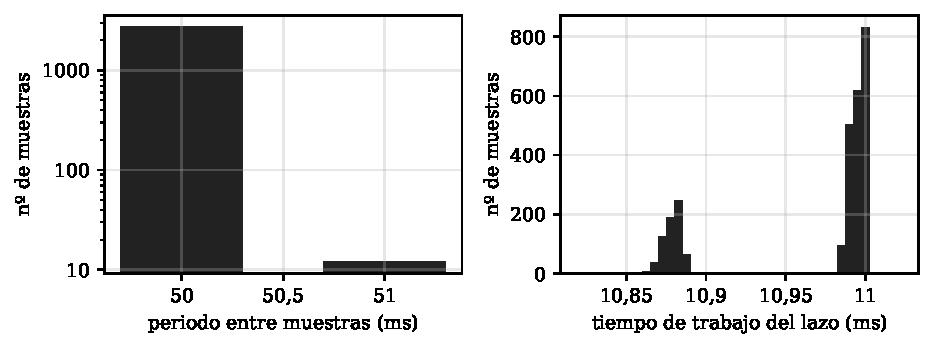
\includegraphics[width=\textwidth]{temporizacion.pdf}
\caption{Izquierda: periodo entre muestras (escala logarítmica). Derecha: tiempo de trabajo por
vuelta del lazo.}
\label{fig:temporizacion}
\end{figure}

\section{Ensayo tipo}

La figura~\ref{fig:ensayo-tipo} muestra el ensayo de las 18:08:46. La secuencia es:

\begin{enumerate}
  \item El eje arranca en B y sube hacia A. Durante la primera media revolución (zona sombreada) la
        señal de la célula permanece plana y el par del motor es de unas \SI{3}{\uacc}: el mecanismo
        está recogiendo holgura y todavía no levanta la masa.
  \item A partir de \SI{0.56}{rev} de avance el par crece con rapidez y la señal de la célula
        empieza a moverse: el cable ya trabaja. Desde ahí hasta A el par sigue creciendo.
  \item Al activarse el final A el ciclo invierte la consigna y el eje baja de vuelta a B, con un par
        menor que en la subida por efecto de las pérdidas.
  \item La repetición se cierra al volver a tocar B. La duración total es de \SI{8.9}{\second}.
\end{enumerate}

\begin{figure}[tbp]
\centering
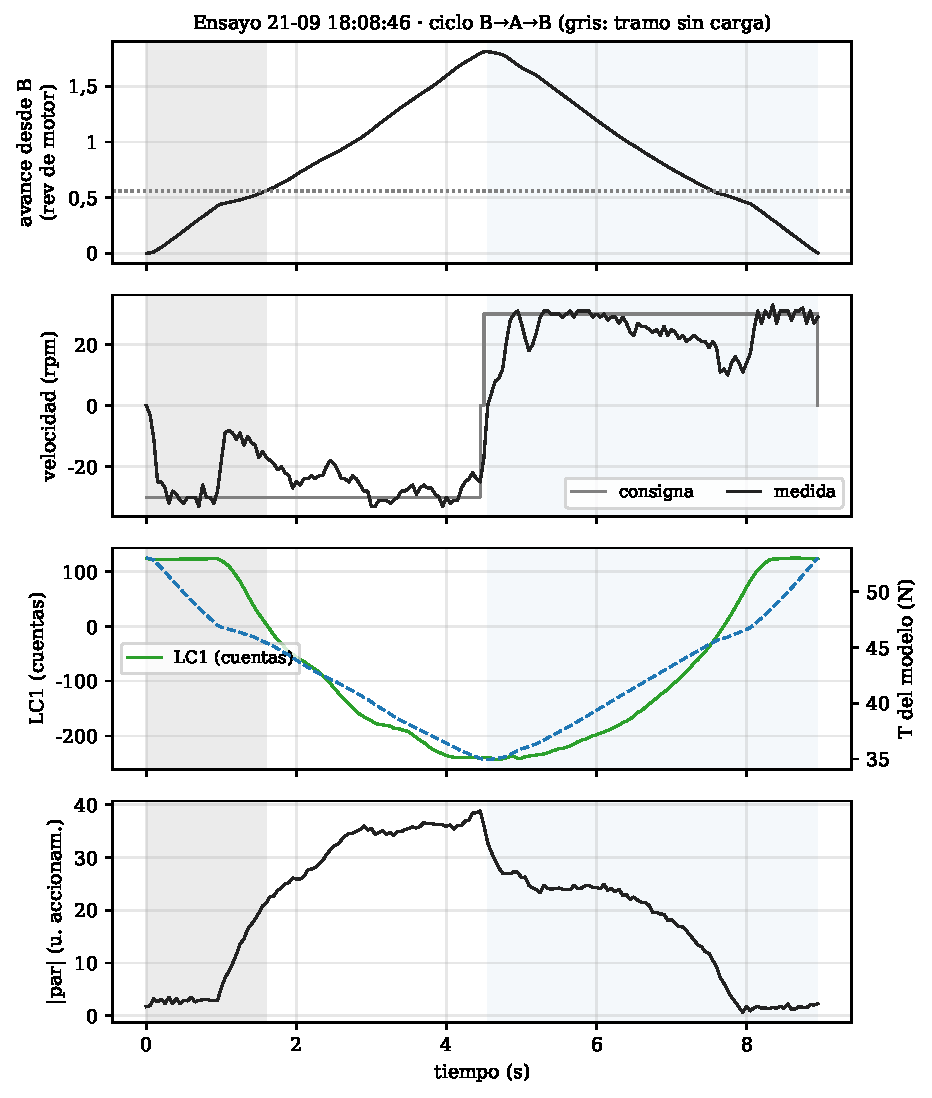
\includegraphics[width=\textwidth]{n_ensayo_tipo.pdf}
\caption{Ensayo tipo de la campaña del 21 de septiembre: avance, velocidad, señal de la célula con
la tensión del modelo superpuesta, y par del motor. En gris, el tramo inicial sin carga.}
\label{fig:ensayo-tipo}
\end{figure}

\section{Repetibilidad}

Los tres ensayos limpios alcanzan el final de carrera A tras \num{1.789}, \num{1.806} y
\SI{1.810}{rev} de avance, con una desviación típica de \SI{11}{mrev}, y vuelven a B con
un avance final de \num{-14}, \num{+5} y \SI{+1}{mrev}. Es decir, el recorrido entre los
dos finales de carrera se repite dentro del \SI{0.6}{\percent}, y el ciclo cierra prácticamente sobre
el punto de partida. El tramo inicial sin carga también es repetible: el par supera las
\SI{10}{\uacc} en \num{0.55}, \num{0.56} y \SI{0.58}{rev}.

La dispersión combina la repetibilidad de los propios finales de carrera con la deriva de la posición
integrada a lo largo de casi dos revoluciones, de modo que es una cota superior de ambas.

\section{Tensión y par a lo largo del recorrido}

La figura~\ref{fig:fuerza-par} superpone las muestras de los tres ensayos limpios en las que el eje
se mueve de forma estable. Se aprecian tres hechos: los ensayos son muy repetibles, la señal de la
célula recorre el mismo camino en subida y bajada (una vez descontado el retardo de su filtro), y el
par es sistemáticamente mayor en la subida que en la bajada, como corresponde a unas pérdidas que se
oponen siempre al movimiento.

\begin{figure}[tbp]
\centering
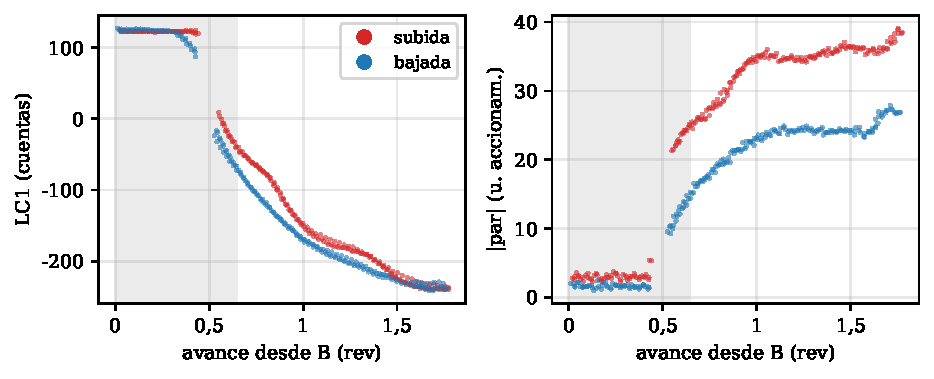
\includegraphics[width=\textwidth]{n_fuerza_par.pdf}
\caption{Señal de la célula (izquierda) y par del motor (derecha) frente al avance, en los tres
ensayos limpios. En gris, el tramo sin carga.}
\label{fig:fuerza-par}
\end{figure}

Aplicando la separación de la ecuación~\eqref{eq:separacion} sobre intervalos de \SI{0.05}{rev}
(figura~\ref{fig:descomposicion}) se obtiene, en el tramo con carga (de \num{0.68} a
\SI{1.73}{rev}):

\begin{itemize}
  \item \textbf{par gravitatorio} $\tau_g$: crece de \num{20.8} a \SI{32.3}{\uacc}, es decir,
        un \SI{+56}{\percent};
  \item \textbf{pérdidas} $\tau_f$: \SI{5.4}{\uacc} de media, el \SI{19}{\percent} de $\tau_g$, y
        prácticamente constantes a lo largo del recorrido, lo que corresponde a un rozamiento de tipo
        Coulomb;
  \item \textbf{tensión del modelo} $T$: \emph{decrece} de \num{44.2} a \SI{35.5}{\newton}, un
        \SI{-20}{\percent}, porque al subir la barra el brazo del cable mejora más deprisa de lo que
        crece el momento del peso.
\end{itemize}

\begin{figure}[tbp]
\centering
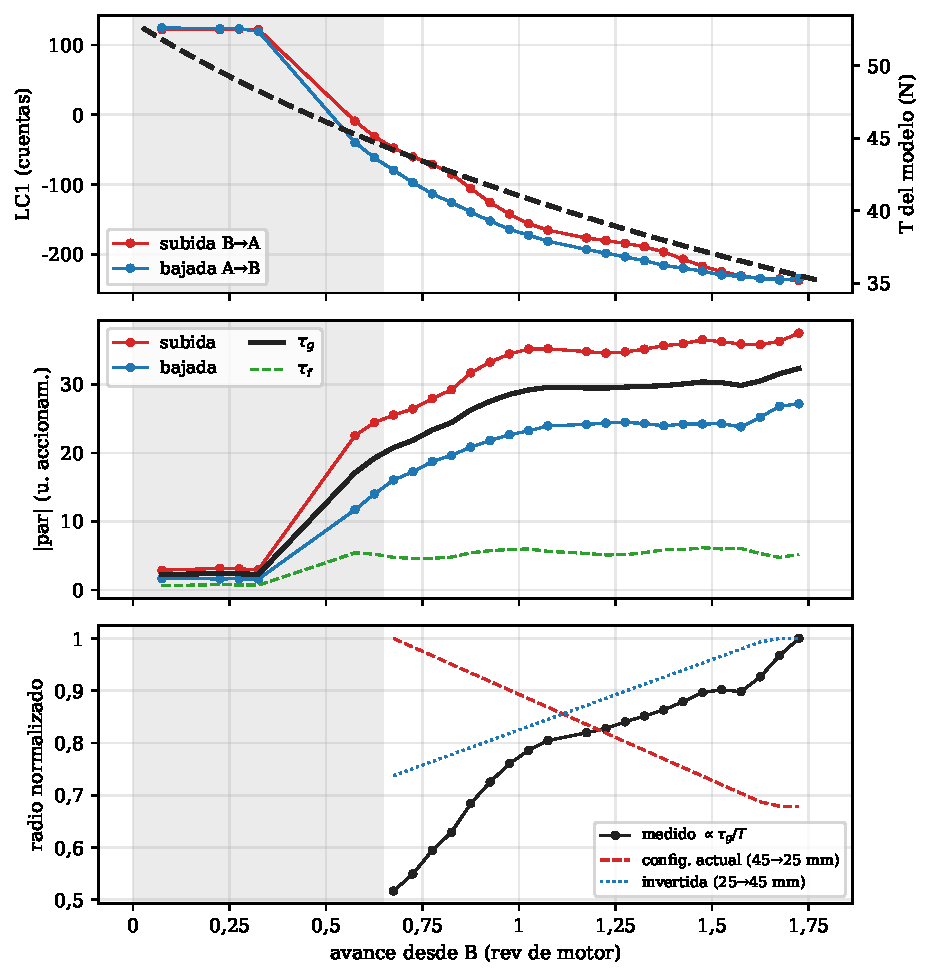
\includegraphics[width=\textwidth]{n_descomposicion.pdf}
\caption{Arriba: señal de la célula en cada sentido, con la tensión del modelo. Centro: par en cada
sentido, componente gravitatoria $\tau_g$ y pérdidas $\tau_f$. Abajo: radio efectivo medido frente a
las dos orientaciones posibles de la caracola.}
\label{fig:descomposicion}
\end{figure}

\section{Contraste con el modelo: cilindro frente a caracola}
\label{sec:res-contraste}

Éste es el núcleo del trabajo experimental. Se comparan tres hipótesis de tambor, todas con la misma
geometría del mecanismo y el mismo recorrido de cable:

\begin{enumerate}
  \item \textbf{cilindro} de radio constante $r = \SI{34.2}{\milli\metre}$, el que paga el mismo
        cable en el mismo giro;
  \item \textbf{caracola configurada}, con el radio decreciendo de \num{45} a \SI{25}{\milli\metre};
  \item \textbf{caracola invertida}, con el radio creciendo de \num{25} a \SI{45}{\milli\metre}.
\end{enumerate}

\subsection{Lo que dice la fuerza: nada concluyente}

La tabla~\ref{tab:contraste} recoge el ajuste de cada hipótesis contra la señal de la célula. Las
tres dan coeficientes de determinación altos, entre \num{0.93} y \num{0.97}. No es que las tres sean
correctas: es que la señal de la célula, sin calibrar, no tiene capacidad para distinguirlas. El
ajuste absorbe en su pendiente tanto la sensibilidad desconocida como el signo
(sección~\ref{sec:mod-ambiguedad}), y lo poco que diferencia a las tres hipótesis en la forma de la
curva queda por debajo del ruido y del retardo del filtro.

\begin{table}[H]
\centering
\caption{Contraste de las tres hipótesis de tambor sobre el tramo con carga. El $R^2$ del par no
distingue el signo; la columna de la pendiente sí: un valor negativo significa que el modelo y la
medida evolucionan en sentidos opuestos.}
\label{tab:contraste}
\small
\begin{tabularx}{\textwidth}{@{}Xccccc@{}}
\toprule
Hipótesis & \multicolumn{2}{c}{Fuerza} & \multicolumn{2}{c}{Par} & Variación de $\tau$ \\
\cmidrule(lr){2-3}\cmidrule(lr){4-5}
 & $R^2$ & pendiente & $R^2$ & pendiente & del modelo \\
\midrule
Cilindro, $r=\SI{34.2}{\milli\metre}$ & 0,947 & $+$ & 0,780 & $-$ & \SI{-22}{\percent} \\
Caracola configurada, 45$\to$25 mm & 0,966 & $+$ & 0,809 & $-$ & \SI{-45}{\percent} \\
Caracola invertida, 25$\to$45 mm & 0,930 & $+$ & 0,673 & $+$ & \SI{+2}{\percent} \\
\midrule
\textbf{Medido} & \multicolumn{4}{c}{} & \textbf{\SI{+56}{\percent}} \\
\bottomrule
\end{tabularx}
\end{table}

\subsection{Lo que dice el par: el tambor no es un cilindro}

El par del accionamiento no necesita calibración, y con él la comparación sí es concluyente. En un
tambor cilíndrico el par es proporcional a la tensión, porque el radio no cambia:
\begin{equation}
  \tau_{\text{cil}}(\varphi) = T(\varphi)\;r_c \quad\Longrightarrow\quad
  \frac{\Delta\tau}{\tau} = \frac{\Delta T}{T} = \SI{-22}{\percent}.
\end{equation}
Es decir, un cilindro obliga al par a \emph{bajar} un \SI{22}{\percent} a lo largo del tramo con
carga. El par medido \emph{sube} un \SI{56}{\percent}. La discrepancia no es de matiz: modelo y
medida evolucionan en sentidos opuestos, y el cociente entre ambos comportamientos es de un factor
\num{2.0} sobre el recorrido.

La conclusión es inmediata: \textbf{el tambor no se comporta como un cilindro}. Y como la única
diferencia entre las dos hipótesis es el radio de enrollamiento, la medida permite estimarlo: el
radio efectivo de la ecuación~\eqref{eq:radio-efectivo} pasa de \num{0.470} a
\SI{0.909}{\uacc\per\newton}, es decir, \textbf{crece un \SI{93}{\percent}} a lo largo del tramo con
carga (figura~\ref{fig:cilindro}).

\begin{figure}[tbp]
\centering
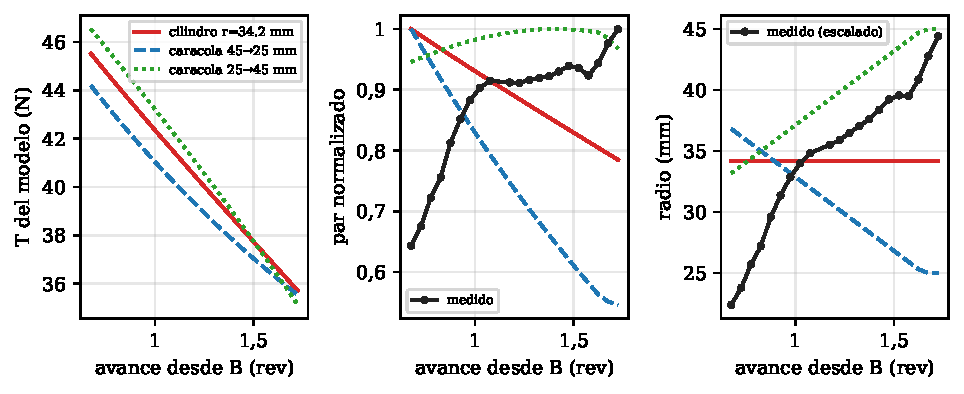
\includegraphics[width=\textwidth]{n_cilindro.pdf}
\caption{Contraste de las tres hipótesis. Izquierda: tensión del modelo. Centro: par normalizado de
cada hipótesis frente al par medido. Derecha: radio de cada hipótesis frente al radio efectivo
deducido de la medida.}
\label{fig:cilindro}
\end{figure}

\subsection{Cuánto compensa, y en qué sentido}

Que el radio crezca es, cualitativamente, lo que pide la compensación: como la tensión baja al subir
la barra, el radio tiene que crecer para que el producto se mantenga. La cuestión es cuánto. Con el
recorrido medido, para que el par fuese exactamente constante bastaría con que el radio creciera un
\SI{24}{\percent}. El radio efectivo crece un \SI{93}{\percent}, casi cuatro veces más.

El resultado, por tanto, tiene dos caras:

\begin{itemize}
  \item \textbf{La caracola actúa, y de forma medible.} Frente al \SI{-22}{\percent} que impondría un
        cilindro, el par real recorre un camino completamente distinto. El mecanismo cambia la
        relación de transmisión a lo largo del recorrido, que es exactamente lo que se quería
        comprobar.
  \item \textbf{Pero no compensa: sobrecompensa.} En lugar de aplanar el par lo empeora en el otro
        sentido, pasando de una caída del \SI{22}{\percent} a una subida del \SI{56}{\percent}. Con
        estos parámetros, el rizado de par sobre el tramo con carga es peor que el de un cilindro
        equivalente (tabla~\ref{tab:perfiles}).
\end{itemize}

Además, el sentido del radio efectivo medido (creciente) es el \emph{contrario} al de la caracola
configurada en el banco (decreciente, de \num{45} a \SI{25}{\milli\metre}), lo que apunta a que la
pieza está descrita al revés en la configuración, montada al revés en la máquina, o ambas cosas
\verificar{medir el perfil real de la caracola y comprobar en qué sentido se enrolla el cable}.

\section{Ajuste de los parámetros del mecanismo}
\label{sec:res-ajuste}

Los parámetros de la tabla~\ref{tab:geometria} no proceden de una medición, sino de un ajuste sobre
los propios ensayos, y conviene ser explícito sobre su alcance. Ajustando sólo contra la señal de la
célula se obtienen los valores que usa la configuración actual, con $R^2 \approx 0{,}93$. Al repetir
el ajuste incluyendo el par, el optimizador se marcha a valores sin sentido físico ---radio final de
\SI{7}{\milli\metre}, desplazamiento de la salida del cable de \SI{200}{\milli\metre}, reducción
\num{3.5}--- aunque mejore formalmente los coeficientes ($R^2$ de \num{0.99} y \num{0.97}).

Esa divergencia es en sí misma un resultado: significa que el modelo, con la parametrización
elegida, no puede reproducir a la vez la fuerza y el par medidos. Faltan datos independientes, y los
que faltan son precisamente los que no se han medido: las cotas del mecanismo y la calibración de la
célula. Mientras no se midan, cualquier juego de parámetros ajustado es una descripción de los datos,
no una verificación del modelo.

\section{Comparación con la campaña preliminar}

La campaña del 14 y 15 de septiembre, analizada con el modelo anterior (salida del cable en la
vertical, tensión proporcional al cable) y con el ciclo A$\rightarrow$B$\rightarrow$A, sugería lo
contrario: en el tramo central del recorrido la tensión variaba un \SI{17}{\percent} y el par
gravitatorio sólo un \SI{6.4}{\percent}, lo que se interpretó como una compensación parcial. Aquel
resultado no se sostiene, por tres motivos que conviene dejar escritos:

\begin{enumerate}
  \item el modelo de tensión era el del caso particular $dx=0$, que no corresponde al montaje;
  \item el sentido del recorrido era el opuesto y el ciclo no empezaba en el extremo del mecanismo,
        de modo que el tramo analizado no es el mismo;
  \item la calibración de la célula que entonces se daba por buena tenía incluso el signo contrario
        al que se deduce ahora, lo que confirma que la fuerza no estaba midiendo lo que se creía.
\end{enumerate}

La lección metodológica es la que recoge la sección~\ref{sec:prob-signo}: un ajuste con buen $R^2$
sobre una única magnitud sin calibrar puede confirmar una hipótesis equivocada.

\section{Limitaciones de las medidas}
\label{sec:res-limitaciones}

\begin{itemize}
  \item \textbf{Célula sin calibrar.} La constante cuentas/newton ha salido distinta en cada intento
        (\num{14.41} en la configuración, \num{20.5} ajustando contra el modelo, \numrange{27}{28} en
        los ensayos limpios) y con signo cambiante entre campañas. Los valores absolutos de fuerza de
        esta memoria son, por tanto, orientativos.
  \item \textbf{Cotas sin medir.} Toda la tensión del modelo depende de $L_2$, $dx$, $L_3$, $L_4$ y
        $\alpha_0$, que son ajustados y no medidos.
  \item \textbf{Escala del par desconocida.} Por eso todos los resultados se expresan en variaciones
        relativas, que no dependen de ella.
  \item \textbf{Tramo sin carga.} La primera media revolución no aporta información y obliga a
        recortar el recorrido analizado.
  \item \textbf{Filtro de la célula.} La media móvil de ocho lecturas introduce un retardo que sólo
        se compensa en primera aproximación al promediar los dos sentidos.
  \item \textbf{Una sola masa y un solo montaje.} No se ha estudiado la dependencia con la carga.
\end{itemize}

\section{Trabajo pendiente para cerrar la validación}

\begin{enumerate}
  \item \textbf{Medir las cotas} del mecanismo ($L_2$, $dx$, $L_3$, $L_4$) y el ángulo de la barra en
        B, e introducirlas en la configuración en lugar de los valores ajustados.
  \item \textbf{Medir el perfil de la caracola}: radios inicial y final, sentido de enrollamiento y
        barrido, que es la magnitud que el análisis deduce de forma indirecta.
  \item \textbf{Calibrar la célula} con masas patrón: escalones crecientes y decrecientes que cubran
        el rango de uso, ajuste por mínimos cuadrados, linealidad, histéresis y repetibilidad, y
        estimación de la incertidumbre con $k=2$.
  \item \textbf{Eliminar la holgura inicial} o, al menos, medirla, para que el recorrido con carga
        sea el recorrido completo.
  \item \textbf{Repetir la campaña} con todo lo anterior y contrastar de nuevo cilindro frente a
        caracola, que es una comparación que el banco ya sabe hacer.
\end{enumerate}


\chapter{Gestión del proyecto}
\label{chap:gestion}

\section{Ciclo de vida}

El proyecto ha seguido un ciclo de vida incremental, con siete iteraciones en las que cada una
entrega algo utilizable y se valida antes de pasar a la siguiente. No es una elección de estilo: en
un trabajo con tanta incertidumbre sobre el mecanismo y los componentes, cada iteración ha servido
para descartar una hipótesis. Las fases de definición y análisis se concentraron en la primera
iteración; el diseño, la construcción y las pruebas se repiten en todas.

La validación se ha apoyado sistemáticamente en programas de prueba por subsistema
(sección~\ref{sec:hw-validacion}), de modo que ningún fallo de integración obligara a depurar todo
el sistema a la vez.

\section{Planificación}

\subsection{Planificación real}

La planificación se ha reconstruido a partir del historial del repositorio: 36 \emph{commits} entre
el 4 de marzo y el 21 de septiembre de 2026, concentrados en nueve semanas
(figura~\ref{fig:actividad-git}). El historial sólo refleja el trabajo sobre código y diseño
electrónico; los periodos sin \emph{commits} corresponden a montaje mecánico, pruebas sin cambios de
código y periodo lectivo \completar{describir las actividades de abril a junio y de julio a agosto}.

\begin{figure}[tbp]
\centering
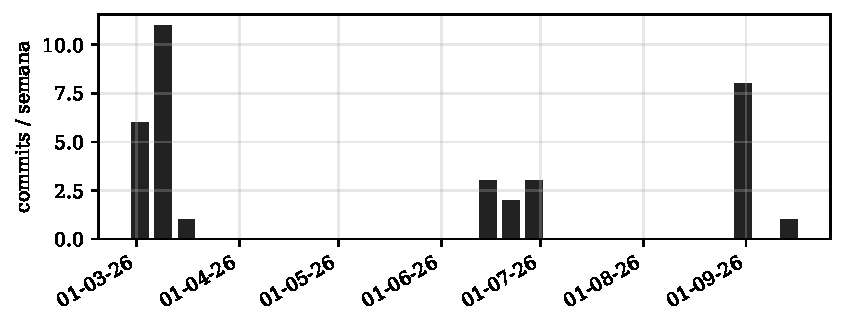
\includegraphics[width=\textwidth]{actividad_git.pdf}
\caption{\emph{Commits} por semana en el repositorio del proyecto.}
\label{fig:actividad-git}
\end{figure}

\begin{description}[style=nextline,leftmargin=1.5em]
  \item[F1. Exploración del accionamiento (2--10 de marzo)] Comunicación Modbus con una placa XIAO
        ESP32-S3: escaneo de direcciones, modos par y velocidad, monitor de terminal, parámetros del
        accionamiento y resistencia de frenado. Culmina en un firmware v1.0 con regulador de fuerza
        en modo par.
  \item[F2. Diseño de la placa adaptadora (12--17 de marzo)] Esquema y colocación de la revisión~A.
  \item[F3. Migración a Raspberry Pi Pico 2 y validación de la placa (20--30 de junio)] Programas de
        prueba de entradas y salidas, células de carga, RS-485 y escaneo Modbus. Versión de doble
        núcleo.
  \item[F4. Firmware de posición en modo velocidad (4 de julio)] Movimiento entre extremos con
        integración de la posición y monitor asociado.
  \item[F5. Firmware v2 y supervisión web (2--6 de septiembre)] \emph{Homing} con dos finales de
        carrera, servidor FastAPI, página de supervisión, ciclos automáticos y grabación de ensayos.
  \item[F6. Primera campaña de ensayos (14--15 de septiembre)] Quince ensayos con el ciclo
        A$\rightarrow$B$\rightarrow$A, visor de ensayos con curva teórica y primer análisis.
  \item[F7. Rediseño del ciclo y del modelo, y segunda campaña (21 de septiembre)] Ciclo
        B$\rightarrow$A$\rightarrow$B con extremos por finales de carrera, modelo con la salida del
        cable desplazada, configuración única del mecanismo con simulador, segunda campaña de
        ensayos y análisis definitivo.
\end{description}

\begin{figure}[tbp]
\centering
\resizebox{\textwidth}{!}{%
\begin{ganttchart}[
    x unit=0.37cm, y unit chart=0.52cm, y unit title=0.55cm,
    vgrid={*1{black!8, dotted}}, hgrid,
    title label font=\scriptsize, bar label font=\scriptsize,
    milestone label font=\scriptsize\itshape,
    bar/.append style={fill=blue!45}, milestone/.append style={fill=red!70},
    bar height=0.55, group label font=\scriptsize\bfseries,
    inline=false
  ]{1}{31}
  \gantttitle{Mar}{5} \gantttitle{Abr}{4} \gantttitle{May}{4} \gantttitle{Jun}{5}
  \gantttitle{Jul}{4} \gantttitle{Ago}{5} \gantttitle{Sep}{4} \\
  \ganttbar{F1 Exploración accionamiento}{1}{2} \\
  \ganttmilestone{Firmware v1.0}{2} \\
  \ganttbar{F2 Diseño PCB rev. A}{2}{3} \\
  \ganttbar[bar/.append style={fill=black!15}]{Actividad fuera de git}{4}{15} \\
  \ganttbar{F3 Migración a Pico 2 y pruebas}{16}{18} \\
  \ganttbar{F4 Firmware de posición}{18}{18} \\
  \ganttbar[bar/.append style={fill=black!15}]{Actividad fuera de git}{19}{26} \\
  \ganttbar{F5 Firmware v2 y web}{27}{28} \\
  \ganttmilestone{Primer ciclo grabado}{28} \\
  \ganttbar{F6 Primera campaña}{29}{29} \\
  \ganttbar{F7 Ciclo y modelo nuevos, 2.ª campaña}{30}{30} \\
  \ganttbar{Redacción de la memoria}{29}{31}
\end{ganttchart}%
}
\caption{Diagrama de Gantt reconstruido (semanas desde el 2 de marzo de 2026).}
\label{fig:gantt}
\end{figure}

\section{Presupuesto}

\subsection{Personal}

La dedicación de un TFG se fija en créditos ECTS, cada uno de 25 a 30 horas de trabajo
\cite{rd1125}. La tabla~\ref{tab:horas} reparte una dedicación estimada por fases \verificar{ajustar
las horas y los créditos del TFG en la titulación}. Para valorar el trabajo se toma como supuesto un
coste de 30~€/h para un ingeniero o ingeniera junior y de 45~€/h para la tutoría.

\begin{table}[H]
\centering
\caption{Dedicación estimada y coste de personal.}
\label{tab:horas}
\begin{tabular}{@{}lrrr@{}}
\toprule
Actividad & Horas & €/h & Coste (€) \\
\midrule
Estudio y documentación & 30 & 30 & 900 \\
Exploración del accionamiento (F1) & 35 & 30 & 1.050 \\
Diseño de la placa (F2) & 45 & 30 & 1.350 \\
Pruebas de placa y comunicaciones (F3) & 45 & 30 & 1.350 \\
Firmware (F4--F5) & 70 & 30 & 2.100 \\
Software de supervisión (F5, F7) & 60 & 30 & 1.800 \\
Ensayos y análisis (F6, F7) & 40 & 30 & 1.200 \\
Redacción de la memoria & 50 & 30 & 1.500 \\
\midrule
Subtotal trabajo técnico & 375 & & 11.250 \\
Tutoría & 25 & 45 & 1.125 \\
\midrule
\textbf{Total recursos humanos} & & & \textbf{12.375} \\
\bottomrule
\end{tabular}
\end{table}

\subsection{Material}

\begin{longtable}{@{}L{0.42\textwidth}rrr@{}}
\caption{Material del sistema.}\label{tab:material}\\
\toprule
Elemento & Cant. & Precio unit. (€) & Total (€) \\
\midrule
\endfirsthead
\toprule
Elemento & Cant. & Precio unit. (€) & Total (€) \\
\midrule
\endhead
Raspberry Pi Pico 2 & 1 & \completar{} & \\
Transceptor RS-485 THVD1400 & 1 & \completar{} & \\
Interruptor de lado alto TPS4H000-Q1 & 1 & \completar{} & \\
Amplificador operacional MCP6294 & 1 & \completar{} & \\
Diodos zéner BZX384 & 4 & \completar{} & \\
Resistencias y condensadores SMD 0805 & 25 & \completar{} & \\
Bornas de tornillo y tiras de pines & -- & \completar{} & \\
Fabricación de la PCB & 1 & \completar{} & \\
Load Cell 2 Click (ZSC31014) & 1 & \completar{} & \\
Célula de carga & 1 & \completar{} & \\
Servomotor paso a paso de lazo cerrado con accionamiento & 1 & \completar{} & \\
Fuente de alimentación del accionamiento & 1 & \completar{} & \\
Finales de carrera & 2 & \completar{} & \\
Caracola, barra, cable, estructura y masa de \SI{2}{\kilo\gram} & -- & \completar{} & \\
\midrule
\textbf{Total material} & & & \completar{} \\
\bottomrule
\end{longtable}

\subsection{Equipos y software}

Todo el software empleado es libre o gratuito (KiCad, Arduino IDE con el núcleo Arduino-Pico,
Python, FastAPI, Chart.js, git y \LaTeX), por lo que su coste es nulo. Los equipos se imputan por
amortización lineal,
\begin{equation}
  A = C\,\frac{t_{\text{uso}}}{t_{\text{vida}}},
\end{equation}
con $C$ el coste de adquisición, $t_{\text{uso}}$ el tiempo de uso y $t_{\text{vida}}$ la vida útil.

\begin{table}[H]
\centering
\caption{Amortización de equipos.}
\label{tab:amortizacion}
\begin{tabular}{@{}lrrrr@{}}
\toprule
Equipo & Coste (€) & Vida útil (meses) & Uso (meses) & Amortización (€) \\
\midrule
Ordenador portátil & \completar{} & 48 & 7 & \\
Polímetro & \completar{} & 60 & 7 & \\
Fuente de laboratorio & \completar{} & 60 & 7 & \\
\midrule
\textbf{Total} & & & & \completar{} \\
\bottomrule
\end{tabular}
\end{table}

\subsection{Resumen de costes}

\begin{table}[H]
\centering
\caption{Presupuesto total.}
\label{tab:presupuesto}
\begin{tabular}{@{}lr@{}}
\toprule
Concepto & Importe (€) \\
\midrule
Recursos humanos & 12.375 \\
Material & \completar{} \\
Amortización de equipos & \completar{} \\
\midrule
Subtotal & \completar{} \\
Costes indirectos (\SI{10}{\percent}, supuesto) & \completar{} \\
\midrule
Base imponible & \completar{} \\
IVA (\SI{21}{\percent}) & \completar{} \\
\midrule
\textbf{Total} & \completar{} \\
\bottomrule
\end{tabular}
\end{table}

\section{Impacto}

\subsection{Impacto técnico y económico}

La consecuencia práctica del capítulo~\ref{chap:modelo} es de dimensionado: para un recorrido dado,
un perfil de par constante reduce el par de pico que debe dar el motor. Sobre el recorrido con carga
de los ensayos, el perfil ideal rebaja el pico un \SI{11}{\percent} respecto a un cilindro
equivalente, lo que permitiría un motor y un accionamiento algo menores. A velocidad constante, las
pérdidas por efecto Joule son proporcionales a $\int\tau^2\,\mathrm{d}\varphi$, mínima cuando el par
es constante (desigualdad de Cauchy-Schwarz), aunque en este caso la mejora es de apenas un
\SI{1}{\percent}.

Esas cifras deben leerse junto con el resultado del capítulo~\ref{chap:resultados}: el tambor
instalado no aplana el par, sino que lo empeora respecto a un cilindro. El margen de mejora que
ofrece el rediseño del perfil es, por tanto, bastante mayor que ese \SI{11}{\percent}.

La plataforma desarrollada es además reutilizable: la placa, el firmware y la aplicación web forman
un banco genérico para cualquier eje accionado por Modbus con medida de fuerza, con un coste de
material muy inferior al de un sistema de adquisición comercial.

\subsection{Objetivos de Desarrollo Sostenible}

\begin{table}[H]
\centering
\caption{Relación del trabajo con los Objetivos de Desarrollo Sostenible \cite{agenda2030}.}
\label{tab:ods}
\begin{tabularx}{\textwidth}{@{}lX@{}}
\toprule
ODS & Contribución \\
\midrule
4. Educación de calidad & Banco de ensayo abierto y documentado, útil como práctica de laboratorio de mecanismos, accionamientos y adquisición de datos. \\
7. Energía asequible y no contaminante & Un perfil de par uniforme reduce las pérdidas en el motor. \\
9. Industria, innovación e infraestructura & Integración de tecnologías industriales (Modbus, RS-485) con herramientas libres de bajo coste. \\
12. Producción y consumo responsables & Dimensionado de actuadores más pequeños; módulo microcontrolador en zócalo, reutilizable; datos brutos conservados para no repetir ensayos. \\
\bottomrule
\end{tabularx}
\end{table}

\subsection{Aspectos éticos, legales y de seguridad}

El prototipo es un equipo de laboratorio que no se comercializa. Su evolución hacia una máquina de
uso por terceros tendría que considerar la Directiva 2006/42/CE de máquinas, que el Reglamento (UE)
2023/1230 sustituye a partir de enero de 2027, la Directiva 2014/30/UE de compatibilidad
electromagnética y la Directiva 2011/65/UE sobre sustancias peligrosas (RoHS). La
sección~\ref{sec:arq-seguridad} discute las limitaciones de seguridad del diseño actual frente a
ISO 13849-1 \cite{iso13849}.

En cuanto a la ética profesional, se ha priorizado la trazabilidad: se conservan las medidas brutas,
las figuras se generan con programas reproducibles y las limitaciones se señalan de forma explícita,
incluso cuando el resultado contradice la hipótesis de partida.


\chapter{Conclusiones}
\label{chap:conclusiones}

\section{Conclusión}

El objetivo general era construir y validar un banco de ensayos para un mecanismo de elevación con
caracola de radio variable, y usarlo para contrastar el modelo del mecanismo. El banco está
construido y funciona; el contraste ha dado un resultado distinto del esperado, y de ahí salen las
conclusiones más interesantes del trabajo.

\subsection{Sobre el banco de ensayos}

\begin{enumerate}
  \item El sistema cumple los requisitos de temporización: muestrea a \SI{20.0}{\hertz} con una
        desviación típica del periodo de \SI{0.06}{\milli\second}, y el trabajo del lazo ocupa el
        \SI{22}{\percent} del periodo. Llegar a ese determinismo exigió abandonar la versión de doble
        núcleo en favor de un lazo de periodo fijo con un único dueño de cada bus.
  \item El ciclo de ensayo B$\rightarrow$A$\rightarrow$B, con los extremos reconocidos por los
        finales de carrera y no por la posición integrada, repite el recorrido dentro del
        \SI{0.6}{\percent} y cierra sobre el punto de partida. Esa decisión hace que el banco sea
        utilizable pese a la incertidumbre de la medida de posición.
  \item Guardar los ensayos en cuentas brutas, con las constantes en la cabecera, ha permitido
        reanalizar por completo dos campañas después de cambiar el modelo y la calibración, sin
        repetir un solo ensayo. Es la decisión de diseño que más ha rendido.
  \item Unificar el modelo en una sola implementación compartida por el simulador y el visor
        eliminó una fuente real de error: las páginas habían divergido hasta calcular con
        geometrías distintas.
\end{enumerate}

\subsection{Sobre el modelo del mecanismo}

\begin{enumerate}\setcounter{enumi}{4}
  \item La posición de la salida del cable respecto a la articulación no es un detalle de dibujo.
        Con la salida en la vertical, la tensión resulta proporcional a la longitud libre de cable,
        un resultado simple y atractivo; con la salida desplazada, esa cancelación desaparece y la
        tensión pasa a depender de dos ángulos. El modelo del banco trabaja ya con el caso general.
  \item El perfil de par constante es el que minimiza el par de pico para un recorrido y un giro de
        tambor dados. La demostración es independiente de la geometría: el trabajo está fijado, luego
        el máximo del par no puede ser menor que su media.
\end{enumerate}

\subsection{Sobre la validación experimental}

\begin{enumerate}\setcounter{enumi}{6}
  \item \textbf{Medir sólo la fuerza no permite validar el modelo.} Con la célula sin calibrar, el
        ajuste incluye la sensibilidad como incógnita y el coeficiente de determinación es el
        cuadrado de la correlación: no distingue el signo. Tres hipótesis de tambor muy distintas
        ---cilindro, caracola y caracola invertida--- ajustan la señal de la célula con
        $R^2$ entre \num{0.93} y \num{0.97}. Un buen ajuste no es una validación.
  \item \textbf{El par del accionamiento sí decide}, porque no depende de ninguna calibración
        pendiente. Y al usarlo, la comparación es concluyente: un tambor cilíndrico obligaría al par
        a bajar un \SI{22}{\percent} a lo largo del tramo con carga, mientras que el par medido sube
        un \SI{56}{\percent}. \textbf{El tambor no se comporta como un cilindro}: su radio efectivo
        crece un \SI{93}{\percent} a lo largo del recorrido.
  \item \textbf{La caracola, sin embargo, no compensa: sobrecompensa.} Para mantener el par constante
        bastaría con que el radio creciera un \SI{24}{\percent}. Con el crecimiento real, el par
        queda peor repartido que con un cilindro equivalente, y además en el sentido contrario al que
        describe la configuración del banco.
  \item Las pérdidas del mecanismo son de tipo Coulomb: constantes a lo largo del recorrido y del
        orden del \SI{19}{\percent} del par gravitatorio.
  \item El resultado anterior no cierra la validación, y es importante decirlo con claridad: mientras
        no se midan las cotas del mecanismo y no se calibre la célula con masas patrón, cualquier
        juego de parámetros es una descripción de los datos y no una verificación del modelo. El
        trabajo deja el procedimiento montado y el diagnóstico hecho.
\end{enumerate}

\subsection{Grado de cumplimiento de los objetivos}

\begin{longtable}{@{}L{0.07\textwidth}L{0.58\textwidth}L{0.25\textwidth}@{}}
\toprule
\textbf{Obj.} & \textbf{Resultado} & \textbf{Estado} \\
\midrule
\endhead
O1 & Modelo estático general, perfil ideal de par constante y demostración de que minimiza el par de pico (capítulo~\ref{chap:modelo}). & Cumplido \\
O2 & Placa adaptadora con RS-485, entradas y salidas y dos zócalos mikroBUS; revisión A analizada y corregida en la revisión B (capítulo~\ref{chap:hardware}). & Cumplido; falta versionar la revisión B \\
O3 & Firmware determinista con Modbus, célula, \emph{homing}, ciclo B$\rightarrow$A$\rightarrow$B y protecciones (capítulo~\ref{chap:firmware}). & Cumplido \\
O4 & Protocolo binario con CRC-8, telemetría por lotes y compatibilidad entre versiones (capítulo~\ref{chap:comunicaciones}). & Cumplido \\
O5 & Servidor y tres páginas web: monitor, configuración con simulador y visor de ensayos (capítulo~\ref{chap:software}). & Cumplido \\
O6 & Caracterización del banco y contraste cilindro/caracola sobre dos campañas (capítulo~\ref{chap:resultados}). & Cumplido; validación abierta a falta de cotas y calibración \\
O7 & Problemas y soluciones, planificación, presupuesto e impacto (capítulos~\ref{chap:problemas} y~\ref{chap:gestion}). & Cumplido \\
\bottomrule
\end{longtable}

\section{Desarrollos futuros}

\subsection{Para cerrar la validación}
\begin{itemize}
  \item Medir las cotas del mecanismo y el perfil real de la caracola (radios, sentido y barrido), y
        sustituir con ellas los parámetros ajustados.
  \item Calibrar la célula de carga con masas patrón y estimar su incertidumbre; con ello, los
        valores de fuerza pasarían de orientativos a trazables.
  \item Confirmar la escala del registro de par del accionamiento para poder expresar los pares en
        \si{\newton\metre}.
  \item Eliminar o medir la holgura inicial del cable, para que el recorrido con carga coincida con
        el recorrido completo.
  \item Repetir la campaña y rehacer el contraste cilindro frente a caracola, que el banco ya
        automatiza.
\end{itemize}

\subsection{Sobre el mecanismo}
\begin{itemize}
  \item Fabricar, por ejemplo por impresión 3D, un tambor cilíndrico y otro con el perfil ideal
        calculado en la sección~\ref{chap:modelo}, y ensayar los tres en el mismo banco. Sería la
        comparación definitiva, con el mecanismo como única variable.
  \item Revisar el sentido de montaje de la caracola actual, que según la medida trabaja al contrario
        de lo que describe la configuración.
  \item Ensayar con varias masas para comprobar la linealidad del modelo con la carga.
\end{itemize}

\subsection{Sobre el sistema de medida}
\begin{itemize}
  \item Leer la posición del codificador del accionamiento por Modbus en lugar de integrar la
        velocidad.
  \item Leer velocidad y par en una sola transacción Modbus (registros 16385 a 16387), lo que
        ahorraría unos \SI{3}{\milli\second} por periodo y permitiría subir la frecuencia de muestreo.
  \item Enviar en cada muestra la posición del firmware y la lectura sin filtrar de la célula, y
        sincronizar la lectura con la señal de interrupción del acondicionador.
  \item Corregir la codificación de la ganancia y los bits de estado del ZSC31014
        (sección~\ref{sec:prob-estado}).
\end{itemize}

\subsection{Sobre la seguridad y la explotación}
\begin{itemize}
  \item Cablear los finales de carrera y una seta de emergencia a la entrada STO del accionamiento,
        de modo que la parada no dependa del software.
  \item Versionar y fabricar la revisión B de la placa, con los ajustes de resistencias propuestos.
  \item Hacer que el servidor escuche sólo en la máquina local o exija autenticación, y añadir
        pruebas automáticas del protocolo.
\end{itemize}

\section{Valoración personal}

\completar{Valoración personal: qué se ha aprendido, qué dificultades han sido más formativas y qué
se haría de otra manera.}


\appendix

\include{capitulos/anexo_pines}

\include{capitulos/anexo_protocolo}

\chapter{Registros Modbus del accionamiento}
\label{anx:modbus}

Dirección = $256\cdot$grupo + índice (índice en hexadecimal). Esclavo 1, 115200 baudios, 8N1.
\verificar{contrastar denominaciones y unidades con el manual del accionamiento}

\begin{longtable}{@{}rllL{0.4\textwidth}r@{}}
\caption{Registros utilizados por el firmware.}\label{tab:registros}\\
\toprule
Dirección & Parámetro & Acceso & Descripción & Valor escrito \\
\midrule
\endfirsthead
\toprule
Dirección & Parámetro & Acceso & Descripción & Valor escrito \\
\midrule
\endhead
0     & C00.00 & E & Modo de control (1 = velocidad, 2 = par) & 1 \\
5     & C00.05 & E & Nivel de rigidez & 10 \\
16    & C00.10 & E & Selección de resistencia de frenado (1 = externa) & 1 \\
17    & C00.11 & E & Potencia de la resistencia de frenado & 1000 \\
18    & C00.12 & E & Valor óhmico de la resistencia de frenado & 235 \\
19    & C00.13 & E & Disipación de la resistencia de frenado & 30 \\
801   & C03.21 & E & Consigna de velocidad (rpm, con signo: negativa hacia A) & cada periodo \\
802   & C03.22 & E & Aceleración & 5 \\
804   & C03.24 & E & Deceleración & 5 \\
1041  & C04.11 & E & Habilitación del servo (0/1) & 0 $\rightarrow$ 1 \\
16385 & 0x4001 & L & Velocidad del motor (rpm) & -- \\
16387 & 0x4003 & L & Par del motor (décimas de \ua) & -- \\
\bottomrule
\end{longtable}

Registros usados en versiones anteriores, con el accionamiento en modo par: 833 (consigna de par,
C03.41), 839 y 840 (límites de par), 1542 (C06.06, apantallamiento de STO) y 1576 (C06.28, retardo
de desconexión tras STO).

\section{Secuencia de configuración}

Al recibir la orden INIT, el firmware escribe en este orden: C04.11 = 0 (deshabilitar), C00.00 = 1
(modo velocidad), C03.21 = 0 (consigna nula), C00.05 (rigidez), C03.22 y C03.24 (rampas), C00.10 a
C00.13 (resistencia de frenado) y C04.11 = 1 (habilitar). Entre escrituras se deja un silencio de
\SI{700}{\micro\second}. Si falla una escritura esencial se repite la secuencia completa, y tras tres
intentos el sistema pasa a estado de error con el código 0x03.


\chapter{Formato de los ficheros de ensayo}
\label{anx:csv}

Cada ensayo se graba en \fichero{cycles/AAAAMMDD-HHMMSS\_ciclo.csv}, codificado en UTF-8. Las líneas
que empiezan por \codigo{\#} forman la cabecera, con las constantes en pares \codigo{clave=valor};
después viene una línea de nombres de columna y una fila por muestra.

\begin{lstlisting}[numbers=none,caption={Comienzo de un fichero de la campaña del 21 de septiembre.}]
# ensayo 2026-09-21 18:08:46
# lc1_cuentas_por_N=14.41  lc1_cero_N=51.78  lc1_int16=0
# repeticiones_pedidas=1  B=1.000 rev (posicion)
# lc1_base ya lleva restada la tara del firmware; lc1_raw es cruda
t_ms,t_rel_s,rep,fase,pos_rev,lc1_raw,lc1_base,rpm,par_x10,ref_rpm,lim_a,lim_b,estado,work_us
\end{lstlisting}

\begin{longtable}{@{}llL{0.58\textwidth}@{}}
\caption{Columnas del fichero de ensayo.}\label{tab:csv}\\
\toprule
Columna & Unidad & Descripción \\
\midrule
\endfirsthead
\toprule
Columna & Unidad & Descripción \\
\midrule
\endhead
t\_ms & ms & Reloj del microcontrolador \\
t\_rel\_s & s & Tiempo desde la primera muestra del ensayo \\
rep & -- & Repetición en curso (desde 1) \\
fase & -- & \codigo{hacia\_A} (subida) o \codigo{volviendo\_a\_B} (bajada). En los ensayos de la campaña preliminar, \codigo{hacia\_B} y \codigo{volviendo\_a\_A} \\
pos\_rev & rev & Posición del eje del motor integrada por el servidor \\
lc1\_raw & cuentas & Lectura bruta del ZSC31014 (una por lote) \\
lc1\_base & cuentas & Media móvil de 8 lecturas menos la tara del firmware \\
rpm & rpm & Velocidad medida por el accionamiento \\
par\_x10 & 0,1\,\ua & Par medido por el accionamiento \\
ref\_rpm & rpm & Consigna de velocidad (negativa hacia A, positiva hacia B) \\
lim\_a, lim\_b & 0/1 & Estado de los finales de carrera \\
estado & -- & Estado de la máquina (tabla~\ref{tab:estados}) \\
work\_us & µs & Tiempo de trabajo de la vuelta del lazo \\
\bottomrule
\end{longtable}

\section{Conversión y análisis}

La conversión a fuerza es $F\,[\si{\newton}] = \text{lc1\_base}/k + F_0$, con $k$ =
\codigo{lc1\_cuentas\_por\_N} y $F_0$ = \codigo{lc1\_cero\_N}. Conviene recordar que esa constante
es provisional (sección~\ref{sec:res-limitaciones}).

Para el análisis, el \emph{avance del ciclo} se obtiene restando la posición de la primera muestra,
que es el punto B donde arranca el ensayo, y corrigiendo el signo con el de la muestra más alejada:
\begin{equation}
  p_i = \big(\text{pos\_rev}_i - \text{pos\_rev}_0\big)\cdot\operatorname{signo}
        \big(\text{pos\_rev}_{\text{lejana}} - \text{pos\_rev}_0\big).
\end{equation}
Así el avance es siempre positivo hacia A, y los ensayos de las dos campañas se pueden comparar pese
a tener sentidos de recorrido opuestos.

\section{Notas sobre las cabeceras}

\begin{itemize}
  \item Los ensayos de la campaña preliminar se grabaron con una versión del servidor que todavía no
        escribía la calibración: en ellos aparece \codigo{lc1\_cuentas\_por\_N=0}.
  \item El texto ``(posicion)'' de la tercera línea se escribe siempre que el recorrido pedido sea
        mayor que cero, aunque el ensayo se haya hecho contra los finales de carrera, que es el caso
        de todos los ensayos de esta memoria. Es un defecto conocido de la cabecera y no afecta a los
        datos.
\end{itemize}


\chapter{Manual de uso}
\label{anx:manual}

\section{Instalación}

\subsection{Firmware}
\begin{enumerate}
  \item Instalar Arduino IDE y añadir en \emph{Preferencias} el gestor de placas de Arduino-Pico:\\
        \url{https://github.com/earlephilhower/arduino-pico/releases/download/global/package_rp2040_index.json}
  \item Instalar el paquete \emph{Raspberry Pi Pico/RP2040/RP2350} y la biblioteca
        \emph{ModbusMaster} desde el gestor de bibliotecas.
  \item Abrir \fichero{firmware\_posicion\_v2/firmware\_posicion\_v2.ino} y seleccionar la placa
        \emph{Raspberry Pi Pico 2}.
  \item Conectar la Pico con el botón BOOTSEL pulsado y cargar el programa.
\end{enumerate}

\subsection{Aplicación de supervisión}
\begin{lstlisting}[language=bash,numbers=none]
python3 -m venv .venv
source .venv/bin/activate
pip install fastapi "uvicorn[standard]" pyserial
python web_monitor.py            # o: python web_monitor.py /dev/ttyACM0
\end{lstlisting}
En Linux, la cuenta de usuario debe pertenecer al grupo \codigo{dialout} para acceder al puerto. La
interfaz se abre en \url{http://localhost:8080}, con tres páginas enlazadas por la barra inferior:
\emph{monitor} (\codigo{/}), \emph{ensayos} (\codigo{/ensayos}) y \emph{mecanismo} (\codigo{/sim}).

\section{Configuración del mecanismo}

Antes de ensayar conviene revisar la geometría en la página \emph{mecanismo}: tipo de tambor
(caracola o cilindro), radios y barrido, reducción, sentido, cotas $L_2$, $dx$, $L_3$, $L_4$, masa y
ángulo $\alpha_0$ en el punto B. Los cambios no se aplican hasta pulsar \emph{Guardar y propagar};
desde ese momento los usan tanto el simulador como el visor de ensayos.

La página avisa si la geometría es imposible (por ejemplo, si el recorrido pedido obligaría a la
barra a pasar de sus topes) e indica, mediante la inversa, cuántas revoluciones de motor hacen falta
para llevar la barra a un ángulo concreto: es el recorrido que tendría que hacer el ciclo.

\section{Procedimiento de ensayo}

\begin{enumerate}
  \item \textbf{Comprobaciones previas}: masa colgada, cable sin cocas y correctamente asentado en la
        caracola, finales de carrera en reposo (indicadores apagados) y zona de movimiento despejada.
  \item \textbf{Inicializar}: pestaña \emph{Servo}, dirección 1, botón \emph{Init}. El estado pasa a
        STOPPED y el indicador del servo a conectado.
  \item \textbf{Homing}: fijar la velocidad de \emph{homing} y el desplazamiento del origen, pulsar
        \emph{Aplicar parámetros} y después \emph{Home}. Al terminar se muestra el recorrido
        A$\rightarrow$B. El eje queda en A, arriba.
  \item \textbf{Tara}: con el mecanismo en reposo, pulsar \emph{Tara} para poner a cero la célula.
  \item \textbf{Ciclo}: en la pestaña \emph{Ciclo B$\rightarrow$A$\rightarrow$B}, elegir hasta dónde
        sube (final de carrera A, recomendado, o una distancia desde B), la velocidad y las
        repeticiones, y pulsar \emph{Iniciar ciclo}. El eje baja primero a B para colocarse ---ese
        tramo no se graba--- y a partir de ahí empieza el ensayo. La grabación se abre y se cierra
        sola.
  \item \textbf{Análisis}: en la página \emph{ensayos}, abrir el fichero y activar la curva teórica
        para compararla con la medida.
  \item \textbf{Fin}: \emph{Shutdown} para deshabilitar el accionamiento.
\end{enumerate}

\section{Programación de la célula de carga}

Con el eje parado, abrir \emph{Configuración avanzada} en la pestaña de la célula, elegir la ganancia
y el cero del A/D y pulsar \emph{Programar}. El eje queda bloqueado cerca de un segundo. El resultado
aparece debajo; si es ``sigue alimentada con el reinicio activo'', usar \emph{Mantener reset} y medir
la tensión de alimentación de la placa Click, que debe caer a \SI{0}{\volt}. Téngase en cuenta que
el código de ganancia de la interfaz no coincide con la ganancia real para los valores intermedios
(sección~\ref{sec:prob-estado}).

\section{Diagnóstico}

\begin{longtable}{@{}L{0.34\textwidth}L{0.6\textwidth}@{}}
\toprule
Síntoma & Causa probable y acción \\
\midrule
\endhead
Servo desconectado, lecturas con código 0xE2 & Tiempo de espera Modbus: revisar el cableado A/B, la masa común, la dirección y la velocidad del accionamiento. Probar con \fichero{test\_modbus\_scan}. \\
Código 0xE3 & CRC incorrecto: ruido o polaridad A/B invertida. \\
Estado ERROR con código 0x03 & Tres fallos de configuración: el accionamiento no acepta las escrituras (¿alimentado?, ¿alarma activa?). \\
Final de carrera siempre activo & Contacto abierto o cable roto (entrada NC). \\
El ciclo termina enseguida y no graba nada & El eje ya estaba en el extremo o la fase de colocación no llegó a B: revisar en \fichero{web\_monitor.log} las líneas de cambio de fase. \\
La interfaz no muestra la fase del ciclo & Firmware y servidor desparejados: recargar el firmware o actualizar el servidor. \\
Célula no válida & Sin lecturas frescas en \SI{150}{\milli\second}: revisar la placa Click y el bus I\textsuperscript{2}C con \fichero{test\_loadcell}. \\
La curva teórica no se parece a la medida & Revisar la geometría en \emph{mecanismo}: el aviso de escala y el de ángulo indican qué parámetro no cuadra. \\
\bottomrule
\end{longtable}

\section{Precauciones}
\begin{itemize}
  \item Las protecciones son de software: mantener las manos fuera del recorrido con el servo
        habilitado y tener a mano el corte de alimentación del accionamiento.
  \item No programar la célula ni usar \emph{Mantener reset} con carga en movimiento (el firmware lo
        impide, pero la medida de fuerza queda interrumpida).
  \item El servidor acepta órdenes de cualquier equipo de la red: usarlo en una red de confianza.
\end{itemize}


\chapter{Estructura del repositorio}
\label{anx:repo}

\begin{longtable}{@{}L{0.38\textwidth}L{0.56\textwidth}@{}}
\toprule
Ruta & Contenido \\
\midrule
\endhead
\multicolumn{2}{@{}l}{\textbf{Firmware}} \\
\fichero{firmware\_posicion\_v2/} & Firmware final (Pico 2): Modbus, célula, \emph{homing}, ciclo B$\rightarrow$A$\rightarrow$B y protocolo. \fichero{i2c\_bus.h}: árbitro del bus I\textsuperscript{2}C. \\
\fichero{firmware\_posicion/} & Versión anterior en modo velocidad entre extremos. \\
\fichero{firmwarerasp/} & Primera versión para Pico 2, con doble núcleo. \\
\fichero{firmware/} & Versión para XIAO ESP32-S3 con regulador de fuerza en modo par. \\
\midrule
\multicolumn{2}{@{}l}{\textbf{Programas de prueba}} \\
\fichero{pcbtest/} & Entradas analógicas, entradas digitales y salidas de potencia. \\
\fichero{test\_limit\_switches/} & Finales de carrera. \\
\fichero{test\_rs485*/}, \fichero{test\_modbus\_scan/} & Bucle local PIO, transmisión, recepción y comunicación Modbus. \\
\fichero{test\_loadcell*/} & ZSC31014 y lectura dual con NAU7802. \\
\fichero{test\_servo\_modbus.py} & Barrido Modbus desde el PC con adaptador USB-RS485. \\
\midrule
\multicolumn{2}{@{}l}{\textbf{Ordenador}} \\
\fichero{web\_monitor.py} & Servidor FastAPI: puente serie-WebSocket, grabación y configuración del mecanismo. \\
\fichero{mecanismo.json} & Geometría del mecanismo (la escribe el servidor). \\
\fichero{static/index.html} & Monitor en tiempo real. \\
\fichero{static/ensayos.html} & Visor de ensayos con curva teórica y ajuste. \\
\fichero{static/sim.html} & Configuración del mecanismo y simulador. \\
\fichero{static/mecanismo.js} & Modelo del mecanismo compartido por las páginas. \\
\fichero{static/tema.css}, \fichero{tema.js}, \fichero{nav.js} & Tema visual, colores de las gráficas y navegación común. \\
\fichero{static/fui/} & Kit de interfaz externo (copia sin modificar). \\
\fichero{leer\_ciclo.py} & Resumen de un ensayo en consola. \\
\fichero{monitor.py}, \fichero{monitor\_posicion.py} & Monitores de terminal de versiones anteriores. \\
\fichero{cycles/} & Ficheros de ensayo (CSV). \\
\midrule
\multicolumn{2}{@{}l}{\textbf{Hardware y documentación}} \\
\fichero{tfg\_adaptador/} & Proyecto KiCad de la placa (revisión A) y copias de seguridad. \\
\fichero{image (1).png} & Esquema de la revisión B. \\
\fichero{README.MD} & Notas sobre la UART de la Pico y el doble núcleo. \\
\fichero{memoria/} & Esta memoria: \fichero{TFG.tex}, \fichero{capitulos/}, \fichero{figuras/} y \fichero{bibliografia/}. \\
\fichero{figuras/generar\_figuras.py} & Figuras y cifras de la campaña preliminar. \\
\fichero{figuras/generar\_figuras21.py} & Figuras y cifras de la campaña del 21 de septiembre. \\
\fichero{figuras/modelo\_mecanismo.py} & Modelo del capítulo~\ref{chap:modelo} portado a Python. \\
\fichero{memoria/\_v1/} & Versión anterior de la memoria, antes de adoptar la plantilla de la ETSIDI. \\
\fichero{old/} & Pruebas iniciales en modo par. \\
\bottomrule
\end{longtable}

\section{Reproducción de los resultados}

Con el repositorio y Python con \codigo{numpy}, \codigo{scipy} y \codigo{matplotlib} instalados:

\begin{lstlisting}[language=bash,numbers=none]
python memoria/figuras/generar_figuras.py     # campaña preliminar
python memoria/figuras/generar_figuras21.py   # campaña del 21 de septiembre
\end{lstlisting}

Ambos programas leen \fichero{cycles/*.csv}, escriben las figuras en \fichero{memoria/figuras/} y
dejan las cifras en \fichero{datos.json} y \fichero{datos21.json}, que son las que cita el
capítulo~\ref{chap:resultados}. Los parámetros del mecanismo están al principio de
\fichero{modelo\_mecanismo.py} y deben coincidir con los de \fichero{mecanismo.json}.


\backmatter

\bibliographystyle{plain}

\cleardoublepage

\addcontentsline{toc}{chapter}{Bibliografia}

\bibliography{bibliografia/bibliografia}

\end{document}
